\documentclass[12pt,a4paper]{report}

% Package
\usepackage[T1]{fontenc}
\usepackage[utf8]{inputenc}
\usepackage[italian]{babel}
\usepackage{graphicx}
\usepackage{geometry}
\geometry{a4paper, margin=2.5cm}
\usepackage{ltablex}
\usepackage{booktabs}
\usepackage{float}
\usepackage{titlesec}
\usepackage{enumitem}
\setlist[itemize]{noitemsep}
\usepackage[table]{xcolor}
\usepackage{array}
\usepackage{listings}

% CARICAMENTO HYPERREF (SEMPRE PER ULTIMO)
\usepackage{hyperref}
\hypersetup{
    colorlinks=false,
    pdfborder={0 0 0},
}

\usepackage[normalem]{ulem}

% Stile per i link esterni (sottolineatura continua)
\let\oldhref\href
\renewcommand{\href}[2]{\oldhref{#1}{\uline{#2}}}
\let\oldurl\url
\renewcommand{\url}[1]{\uline{\oldurl{#1}}}

% Stile per i riferimenti interni (sottolineatura a puntini)
\let\oldref\ref
\renewcommand{\ref}[1]{\dotuline{\oldref{#1}}}
\let\oldhyperref\hyperref
\renewcommand{\hyperref}[2][]{\oldhyperref[#1]{\dotuline{#2}}}

% Contatore per i requisiti (permette link precisi nelle tabelle)
\makeatletter
\newcounter{reqcount}
\newcommand{\reqlabel}[1]{%
    \leavevmode\Hy@raisedlink{\refstepcounter{reqcount}\label{#1}}%
    \ignorespaces
}
\makeatother

% SCELTA DEL FONT
\usepackage{lmodern} % Latin Modern (versione migliorata del default LaTeX)
% \usepackage{newtxtext,newtxmath} % Times New Roman (Serif classico, molto formale)
% \usepackage{newpxtext,newpxmath} % Palatino (Serif elegante, ottimo per tesi e report)
% \usepackage[scaled]{helvet} \renewcommand{\familydefault}{\sfdefault} % Helvetica/Arial (Senza grazie)
% \usepackage[sfdefault]{roboto} % Roboto (Moderno, lineare). Se non compila, va installato 'texlive-fonts-extra'.

% Definizione Colori
\definecolor{studyColor}{HTML}{f78a88}
\definecolor{linkColor}{HTML}{4f7ca7}
\definecolor{codeKeyword}{RGB}{0, 0, 255}
\definecolor{codeString}{RGB}{206, 49, 29}
\definecolor{codeComment}{RGB}{0, 128, 0}
\definecolor{codeAttribute}{RGB}{43, 145, 175}
\definecolor{codeBackground}{RGB}{250, 250, 250}

% Configurazione listings per C#
\lstset{
    language=[Sharp]C,
    basicstyle=\ttfamily\small,
    keywordstyle=\color{codeKeyword},
    stringstyle=\color{codeString},
    commentstyle=\color{codeComment},
    numberstyle=\tiny\color{gray},
    numbers=left,
    numbersep=8pt,
    backgroundcolor=\color{codeBackground},
    frame=single,
    rulecolor=\color{lightgray},
    breaklines=true,
    showstringspaces=false,
    tabsize=4,
    morekeywords={var, string, Assert, CollectionAssert, TestFixture, SetUp, Test, DateTime, Profilo, Evento, Indirizzo, Orario, TipoDiLuogo, Commento, Chat},
    literate={à}{{\`a}}1 {è}{{\`e}}1 {ì}{{\`i}}1 {ò}{{\`o}}1 {ù}{{\`u}}1,
}

% Impostazioni
\keepXColumns
\setcounter{secnumdepth}{4}
\setcounter{tocdepth}{2}

% Capitoli
\titleformat{\chapter}
    {\normalfont\Large\bfseries\color{linkColor}}{\thechapter.\ }{0pt}{\Large}
\titlespacing*{\chapter}{0pt}{-20pt}{15pt}

% Sezioni
\titleformat{\section}
    {\normalfont\large\bfseries\color{studyColor}}{\thesection.\ }{0pt}{\large}
\titlespacing*{\section}{0pt}{10pt}{10pt}

% Sottosezioni
\titleformat{\subsection}
    {\normalfont\normalsize\bfseries\color{linkColor}}{\thesubsection.\ }{0pt}{\normalsize} 
\titlespacing*{\subsection}{0pt}{8pt}{8pt}

% Sottosottosezioni
\titleformat{\subsubsection}
    {\normalfont\normalsize\bfseries\color{studyColor}}{\thesubsubsection.\ }{0pt}{\normalsize} 
\titlespacing*{\subsubsection}{0pt}{6pt}{2pt}

% Paragrafi (Sotto-sotto-sottosezioni)
\titleformat{\paragraph}
    {\normalfont\normalsize\bfseries\color{linkColor}}{\theparagraph.\ }{0pt}{\normalsize}
\titlespacing*{\paragraph}{0pt}{10pt}{4pt}


% Tabelle
\renewcommand{\arraystretch}{1.5}
\setlength{\tabcolsep}{10pt}
\setlength{\intextsep}{5pt}
\setlength{\LTpre}{0pt}
\setlength{\LTpost}{0pt}


% Inizio documento
\begin{document}

% Frontepagina
\begin{titlepage}
    \pagenumbering{gobble}
    \centering
    \vspace*{1cm}
    
\includegraphics[width=0.45\textwidth]{images/logo.png}\par
    \vspace{2cm}
    {\fontsize{45}{54}\selectfont\bfseries \textcolor{studyColor}{Study}\textcolor{linkColor}{Link} \par}
    \vfill
    \begin{flushright}
        {\large \textbf{Gruppo 31} \quad A.A. 2025/2026 \par}
        \vspace{0.5cm}
        Matteo Gattobigio \quad 0001117104 \\
        Lucilla Lucchi \quad 0001116767 \\
        Federico Porpora \quad 0001114450 \par
    \end{flushright}
\end{titlepage}

% Abstract
\newpage
\pagenumbering{arabic}
\chapter*{Abstract}
\addcontentsline{toc}{chapter}{Abstract}
Il progetto \textbf{StudyLink} è un'applicazione nata per aiutare gli studenti universitari a trovare e formare gruppi di studio dal vivo, rendendo semplicissimo l'incontro tra colleghi.

La piattaforma punta tutto sulla trasparenza: ogni studente ha un Profilo personale chiaro e visibile.
L'applicazione gestisce le sessioni di studio in modo flessibile, permettendo agli Utenti di alternarsi in due ruoli chiave:
\begin{itemize}
    \item \textbf{L'Organizzatore}, che prende l'iniziativa e crea l'Evento scegliendo la data, l'orario, il luogo d'incontro e i posti disponibili;
    \item \textbf{Il Partecipante}, che sfoglia la Bacheca e si prenota per i gruppi già avviati occupando i posti liberi.
\end{itemize}

Inoltre, per facilitare l'organizzazione, tutti gli iscritti a un Evento hanno a disposizione una Chat di gruppo dedicata. È uno spazio comodo e privato per scambiarsi appunti, materiali di studio o mettersi d'accordo sui dettagli prima di vedersi di persona.

% Indice
\newpage
\tableofcontents

% Analisi dei requisiti
\newpage
\chapter{Analisi dei requisiti}

% Raccolta dei requisiti
\section{Raccolta dei requisiti}
\begin{itemize}[leftmargin=*]
    \item Il sistema deve permettere all'Utente di registrarsi fornendo le proprie Credenziali (Email e Password). La Registrazione è permessa esclusivamente a Utenti aventi un'Email istituzionale universitaria (es. @studio.unibo.it).
    \item Ogni Utente può gestire il proprio Profilo personale, contenente nome, cognome, Corso di studi, una breve Biografia e opzionalmente un'immagine.
    \item Qualsiasi Utente autenticato può creare un nuovo Evento.
    \item L'Organizzatore, nella creazione di un Evento, deve definire:
    \begin{itemize}
        \item \textbf{Titolo:} il titolo dell'Evento deve essere chiaro e descrittivo, nel caso anche della materia che si intende studiare nell'incontro;
        \item \textbf{Data e orario:} l'Evento deve avere una data e un orario di inizio e fine ben definiti;
        \item \textbf{Indirizzo:} indicazione fisica specifica (via, nome della struttura o aula) in cui si terrà l'incontro;
        \item \textbf{Tipo di Luogo:} scegliere tra Luogo ``Pubblico'' o ``Privato'';
        \item \textbf{Numero di posti:} può essere a posti ``Limitati'' o ``Illimitati''.
    \end{itemize}
    \item Il sistema deve offrire una Bacheca globale dove l'Utente può sfogliare gli Eventi di studio creati da altri Utenti. Gli Eventi scompaiono dalla Bacheca una volta pieni.
    \item L'Utente deve poter filtrare gli Eventi in Bacheca in base alla Materia (Specifico per Esame o Generale), Tipo di Luogo (Pubblico o Privato), numero di posti (Limitato o Illimitato) e data. Inoltre, l'utente deve poter inserire un indirizzo personalizzato a sua scelta e un raggio massimo espresso in chilometri per limitare la ricerca.
    \item Gli utenti scelgono l'evento in base al titolo dato dall'organizzatore
    \item Un Utente può prenotarsi per un Evento esistente se sono presenti posti disponibili.
    \item Un Partecipante può annullare la propria Prenotazione fino a un'ora prima, liberando il posto per altri Utenti.
    \item L'Organizzatore può modificare i dettagli dell'Evento o cancellarlo fino all'ora precedente.
    \item L'Organizzatore può rimuovere gli Utenti Partecipanti a sua discrezione.
    \item Alla pubblicazione di un Evento, il sistema deve generare automaticamente una Chat di gruppo privata, accessibile esclusivamente all'Organizzatore e ai Partecipanti di quello specifico Evento.
    \item Al termine dell'Evento i Partecipanti possono lasciare dei Commenti positivi o negativi.
    \item L'interfaccia Utente deve essere intuitiva e ottimizzata per l'uso in mobilità (mobile-friendly), facilitando la navigazione rapida tra Bacheca e Chat.
    \item Le informazioni del Profilo devono essere facilmente consultabili prima di unirsi a un gruppo per favorire un clima di fiducia tra colleghi.
    \item I messaggi scambiati nella Chat devono essere visibili solo ai membri del gruppo di studio corrente. I dati personali devono essere trattati in conformità con le normative vigenti (\href{https://gdpr-info.eu/}{GDPR}).
\end{itemize}

% Requisiti di sistema
\newpage
\section{Requisiti di sistema}

\subsection{Requisiti funzionali}
\begin{tabularx}{\textwidth}{|p{1.2cm}|X|p{2.6cm}|}
    \hline
    \rowcolor{studyColor} \textbf{ID} & \textbf{Requisito} & \textbf{Tipo} \\ \hline
    \endhead
    \reqlabel{R01F}R01F & La Registrazione è ammessa solo tramite Email istituzionale & Funzionale \\ \hline
    \reqlabel{R02F}R02F & Una persona può registrarsi, creando un Profilo Utente & Funzionale \\ \hline
    \reqlabel{R03F}R03F & Un Profilo Utente è accessibile tramite Mail istituzionale e Password & Funzionale \\ \hline
    \reqlabel{R04F}R04F & Un Profilo Utente ha le seguenti informazioni: nome, cognome, Corso di studi, Bio, immagine opzionale e Commenti ricevuti & Funzionale \\ \hline
    \reqlabel{R05F}R05F & Le caratteristiche di un Evento sono: titolo, Tipo di Luogo, data, orario, Indirizzo, posti disponibili & Funzionale \\ \hline
    \reqlabel{R06F}R06F & La Materia di un Evento può essere specificata o generica & Funzionale \\ \hline
    \reqlabel{R07F}R07F & Il tipo di accesso all'Evento è aperto a tutti, chiunque può scegliere di aggiungersi, posti permettendo & Funzionale \\ \hline
    \reqlabel{R08F}R08F & Il numero di posti disponibili può essere limitato o illimitato & Funzionale \\ \hline
    \reqlabel{R09F}R09F & Gli Eventi hanno due fasi: programmato e concluso & Funzionale \\ \hline
    \reqlabel{R10F}R10F & Gli Utenti visualizzano una Bacheca globale di Eventi programmati con almeno un posto disponibile & Funzionale \\ \hline
    \reqlabel{R11F}R11F & Gli Utenti possono filtrare gli Eventi dalla Bacheca per: Tipo di Luogo, data, numero posti, e distanza chilometrica a partire da un indirizzo specifico & Funzionale \\ \hline
    \reqlabel{R12F}R12F & Un Utente può prenotarsi a un Evento, diventandone Partecipante & Funzionale \\ \hline
    \reqlabel{R13F}R13F & Un Utente prima di prenotarsi a un Evento può visualizzare il Profilo Utente dei Partecipanti & Funzionale \\ \hline
    \reqlabel{R14F}R14F & Un Partecipante può annullare la Prenotazione all'Evento fino a un'ora prima dell'inizio & Funzionale \\ \hline
    \reqlabel{R15F}R15F & L'Organizzatore può modificare i dettagli dell'Evento o cancellarlo fino all'ora precedente & Funzionale \\ \hline
    \reqlabel{R16F}R16F & L'Organizzatore può rimuovere i Partecipanti all'Evento a sua discrezione & Funzionale \\ \hline
    \reqlabel{R17F}R17F & Per ogni Evento è prevista una Chat di gruppo accessibile solo ai Partecipanti & Funzionale \\ \hline
    \reqlabel{R18F}R18F & Al termine dell'Evento, ciascun Partecipante può lasciare un Commento a ognuno degli altri presenti & Funzionale \\ \hline
    \reqlabel{R19F}R19F & Un Utente può richiedere l'eliminazione del proprio Profilo & Funzionale \\ \hline
\end{tabularx}

\subsection{Requisiti non funzionali}
\begin{tabularx}{\textwidth}{|p{1.2cm}|X|p{2.6cm}|}
    \hline
    \rowcolor{studyColor} \textbf{ID} & \textbf{Requisito} & \textbf{Tipo} \\ \hline
    \endhead
        \reqlabel{R01N}R01N & La piattaforma deve essere accessibile online & Non funzionale \\ \hline
        \reqlabel{R02N}R02N & Le Credenziali di un Utente sono univoche & Non funzionale \\ \hline
        \reqlabel{R03N}R03N & L'interfaccia della Bacheca deve essere essenziale ed intuitiva & Non funzionale \\ \hline
        \reqlabel{R04N}R04N & Il fuso orario usato dall'applicazione è GMT+1 & Non funzionale \\ \hline
        \reqlabel{R05N}R05N & Il formato di data e orario è gg/mm/aa e hh:mm 24h & Non funzionale \\ \hline
        \reqlabel{R06N}R06N & L'applicazione deve rispettare le norme definite nel \href{https://gdpr-info.eu/}{GDPR} & Non funzionale \\ \hline
        \reqlabel{R07N}R07N & La Bacheca globale deve essere costantemente aggiornata & Non funzionale \\ \hline
        \reqlabel{R08N}R08N & La Password scelta dall'Utente deve essere di almeno 8 caratteri e contenere almeno un numero e un carattere speciale (\#@?!\_-) & Non funzionale \\ \hline
        \reqlabel{R09N}R09N & La ricezione ed invio dei Messaggi deve essere istantanea & Non funzionale \\ \hline
        \reqlabel{R12N}R12N & L'applicazione deve poter operare in totale autonomia senza l'intervento attivo di amministratori umani, garantendo così una maggiore tutela della privacy degli utenti & Non funzionale \\ \hline
\end{tabularx}

% Analisi del dominio
\newpage
\section{Analisi del dominio}

\subsection{Vocabolario}
\begin{tabularx}{\textwidth}{|p{2.8cm}|X|p{2.2cm}|}
    \hline
    \rowcolor{studyColor} \textbf{Voce} & \textbf{Definizione} & \textbf{Sinonimi} \\ \hline
    \endhead
    Profilo & Insieme delle informazioni personali e accademiche che rappresentano l'identità di un Utente all'interno della piattaforma & Account \\ \hline
    Registrazione & Creazione di un Profilo da parte di uno studente & \\ \hline
    Utente & Studente che ha eseguito la Registrazione & \\ \hline
    Autenticazione & Processo tramite il quale uno studente si identifica e si associa al proprio Profilo & Accesso, Login \\ \hline
    Informazioni del Profilo & Dati inseriti dall'Utente, quali nome, cognome, Email, Corso di studi, Biografia ed eventualmente un'immagine & \\ \hline
    Password & Sequenza di caratteri segreta & \\ \hline
    Credenziali & Coppia di Email e Password & \\ \hline
    Evento & Sessione di studio programmata da un Utente, caratterizzata da un titolo, un Indirizzo, un Tipo di Luogo, una data e un orario & Sessione di studio \\ \hline
    Titolo & Nome descrittivo dell'Evento & Nome \\ \hline
    Luogo Pubblico & Luogo fisico accessibile a tutti in cui si svolge un Evento (es. biblioteca, aula studio) & \\ \hline
    Luogo Privato & Luogo fisico privato in cui si svolge un Evento & \\ \hline
    Indirizzo & Indicazione fisica specifica (via, nome della struttura o aula) in cui si terrà l'incontro & Posizione, luogo \\ \hline
    Evento a posti Limitati & Tipologia di Evento che prevede un numero massimo di partecipanti & \\ \hline
    Evento a posti Illimitati & Tipologia di Evento che non prevede un numero massimo di partecipanti & \\ \hline
    Bacheca & Sezione in cui è possibile visualizzare l'elenco degli Eventi disponibili & \\ \hline
    Organizzatore & Utente che crea, gestisce, coordina ed è Partecipante a un Evento & \\ \hline
    Partecipante & Utente che sceglie di unirsi a un Evento & Iscritto \\ \hline
    Prenotazione & Iscrizione a un Evento & Partecipazione, iscrizione \\ \hline
    Filtro & Funzionalità di ricerca che permette di restringere la visualizzazione degli Eventi in Bacheca secondo criteri specifici & \\ \hline
    Commento & Valutazione espressa dai Partecipanti su un altro Partecipante & Recensione \\ \hline
    Chat & Canale di comunicazione testuale privato, creato automaticamente per ogni Evento e riservato ai suoi Partecipanti & Chat condivisa, Chat di gruppo \\ \hline
    Messaggio & Singola comunicazione testuale inviata da un Partecipante all'interno della Chat di gruppo & \\ \hline
\end{tabularx}

% Analisi dei requisiti
\newpage
\section{Analisi dei requisiti}

\subsection{Modello dei casi d'uso}
L'analisi dei requisiti e del dominio hanno portato ai seguenti casi d'uso che interagiscono fra di loro come descritto nel seguente schema.

\begin{figure}[H]
    \centering
    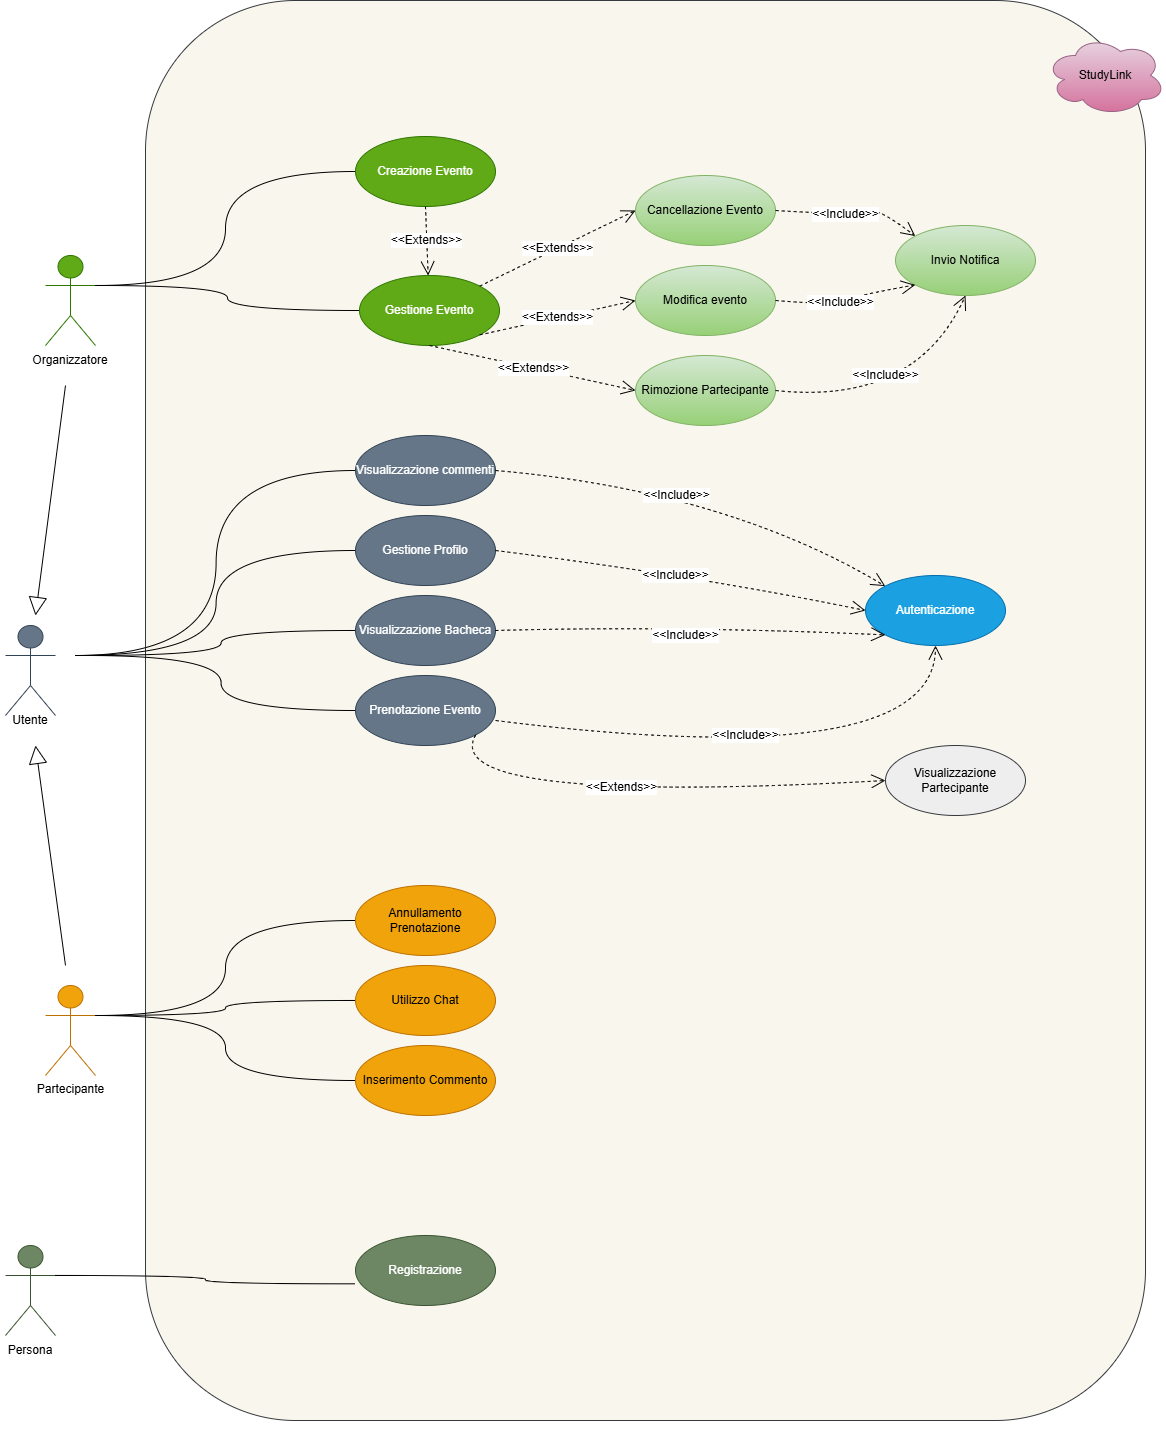
\includegraphics[width=\textwidth,height=0.5\textheight,keepaspectratio]{images/modello-dei-casi-d-uso.png}
    \caption{Modello dei casi d'uso}
\end{figure}
%
\newpage
\subsection{Scenari}
Di seguito sono presentati tutti gli scenari nel loro dettaglio.

\subsubsection{Registrazione}
\reqlabel{tab:Registrazione}
\begin{tabularx}{\textwidth}{|p{3.8cm}|X|}
    \hline
    \rowcolor{studyColor} \textbf{Titolo} & \textbf{Registrazione} \\ \hline
    \endhead
    \textbf{Descrizione} & Procedura di creazione di un account Utente \\ \hline
    \textbf{Attori} & Studente \\ \hline
    \textbf{Relazioni} & \\ \hline
    \textbf{Precondizioni} & \\ \hline
    \textbf{Postcondizioni} & Il sistema memorizza il nuovo Utente \\ \hline
    \textbf{Scenario principale} &
        \begin{enumerate}[nosep, leftmargin=*, before={\vspace{-0.5\baselineskip}}, after={\vspace{-0.8\baselineskip}}]
            \item Il sistema richiede i dati per la registrazione
            \begin{itemize}[nosep, leftmargin=*]
                \item Email
                \item Password
            \end{itemize}
            \item L'attore inserisce i dati richiesti
            \item Il sistema verifica la validità delle credenziali
            \item Il sistema crea il nuovo Utente
        \end{enumerate} \\ \hline
    \textbf{Scenari alternativi} & 
        \begin{itemize}[nosep, leftmargin=*, before={\vspace{-0.5\baselineskip}}, after={\vspace{-0.8\baselineskip}}]
            \item L'Email fornita è già in uso
            \begin{enumerate}[nosep, leftmargin=*]
                \setcounter{enumi}{3}
                \item Il sistema informa l'Utente che la Email è già registrata
                \item Viene mostrata la schermata di autenticazione
            \end{enumerate}
            \item La Password non è sicura
            \begin{enumerate}[nosep, leftmargin=*]
                \setcounter{enumi}{3}
                \item Viene mostrato un messaggio di errore
                \item Lo studente può inserire una nuova Password
            \end{enumerate}
            \item La Email non è istituzionale
            \begin{enumerate}[nosep, leftmargin=*]
                \setcounter{enumi}{3}
                \item Viene mostrato un messaggio di errore
                \item Lo studente può inserire una nuova Email
            \end{enumerate}
        \end{itemize} \\ \hline
    \textbf{Requisiti non funzionali} & \hyperref[R02N]{R02N}, \hyperref[R06N]{R06N}, \hyperref[R08N]{R08N} \\ \hline
    \textbf{Punti aperti} & \\ \hline
\end{tabularx}

\newpage
\subsubsection{Autenticazione}
\reqlabel{tab:Autenticazione}
\begin{tabularx}{\textwidth}{|p{3.8cm}|X|}
    \hline
    \rowcolor{studyColor} \textbf{Titolo} & \textbf{Autenticazione} \\ \hline
    \endhead
    \textbf{Descrizione} & L'Utente inserisce le proprie Credenziali e si autentica sulla piattaforma \\ \hline
    \textbf{Attori} & Utente \\ \hline
    \textbf{Relazioni} &
        \begin{itemize}[nosep, leftmargin=*, before={\vspace{-0.5\baselineskip}}, after={\vspace{-0.8\baselineskip}}]
            \item \hyperref[tab:Visualizzazione Commenti]{Visualizzazione Commenti}
            \item \hyperref[tab:Gestione Profilo]{Gestione Profilo}
            \item \hyperref[tab:Visualizzazione Bacheca]{Visualizzazione Bacheca}
            \item \hyperref[tab:Prenotazione Evento]{Prenotazione Evento}
            \item \hyperref[tab:Creazione Evento]{Creazione Evento}
            \item \hyperref[tab:Gestione Evento]{Gestione Evento}
            \item \hyperref[tab:Rimozione Partecipante]{Rimozione Partecipante}
            \item \hyperref[tab:Annullamento Prenotazione]{Annullamento Prenotazione}
            \item \hyperref[tab:Utilizzo Chat]{Utilizzo Chat}
            \item \hyperref[tab:Inserimento Commento]{Inserimento Commento}
        \end{itemize} \\ \hline
    \textbf{Precondizioni} & L'Utente è registrato nel sistema \\ \hline
    \textbf{Postcondizioni} & L'Utente è autenticato nel sistema \\ \hline
    \textbf{Scenario principale} &
        \begin{enumerate}[nosep, leftmargin=*, before={\vspace{-0.5\baselineskip}}, after={\vspace{-0.8\baselineskip}}]
            \item Il sistema richiede l'inserimento delle Credenziali di accesso
            \item L'Utente inserisce le proprie credenziali
            \item Il sistema verifica che le credenziali appartengano a un Utente
            \item L'Utente è autenticato nel sistema
        \end{enumerate} \\ \hline
    \textbf{Scenari alternativi} & 
        \begin{itemize}[nosep, leftmargin=*, before={\vspace{-0.5\baselineskip}}, after={\vspace{-0.8\baselineskip}}]
            \item Le Credenziali sono errate
            \begin{enumerate}[nosep, leftmargin=*]
                \setcounter{enumi}{3}
                \item Viene mostrato un messaggio di errore
                \item L'Utente può reinserire le Credenziali
            \end{enumerate}
        \end{itemize} \\ \hline
    \textbf{Requisiti non funzionali} & \hyperref[R02N]{R02N} \\ \hline
    \textbf{Punti aperti} & \\ \hline
\end{tabularx}

\newpage
\subsubsection{Gestione profilo}
\reqlabel{tab:Gestione Profilo}
\begin{tabularx}{\textwidth}{|p{3.8cm}|X|}
    \hline
    \rowcolor{studyColor} \textbf{Titolo} & \textbf{Gestione profilo} \\ \hline
    \endhead
    \textbf{Descrizione} & Inserimento, modifica o eliminazione di dati specifici dell'Utente \\ \hline
    \textbf{Attori} & Utente \\ \hline
    \textbf{Relazioni} &
        \begin{itemize}[nosep, leftmargin=*, before={\vspace{-0.5\baselineskip}}, after={\vspace{-0.8\baselineskip}}]
            \item \hyperref[tab:Autenticazione]{Autenticazione}
        \end{itemize} \\ \hline
    \textbf{Precondizioni} & \\ \hline
    \textbf{Postcondizioni} & Le modifiche del profilo sono memorizzate nel sistema \\ \hline
    \textbf{Scenario principale} &
        \begin{enumerate}[nosep, leftmargin=*, before={\vspace{-0.5\baselineskip}}, after={\vspace{-0.8\baselineskip}}]
            \item \hyperref[tab:Autenticazione]{Autenticazione}
            \item Il sistema mostra le funzionalità disponibili:
            \begin{enumerate}[nosep, leftmargin=*]
                \item Inserire e modificare i propri dati come:
                \begin{itemize}[nosep, leftmargin=*]
                    \item Nome
                    \item Cognome
                    \item Password
                    \item Corso di studi
                    \item Biografia
                    \item Immagine
                \end{itemize}
                \item Eliminare l'account dal sistema
            \end{enumerate}
            \item Il sistema apporta le modifiche effettuate
        \end{enumerate} \\ \hline
    \textbf{Scenari alternativi} & 
        \begin{itemize}[nosep, leftmargin=*, before={\vspace{-0.5\baselineskip}}, after={\vspace{-0.8\baselineskip}}]
            \item La Password non è sicura
            \begin{enumerate}[nosep, leftmargin=*]
                \setcounter{enumi}{2}
                \item Viene mostrato un messaggio di errore
                \item L'Utente può inserire una nuova Password
            \end{enumerate}
            \item La Biografia è troppo lunga
            \begin{enumerate}[nosep, leftmargin=*]
                \setcounter{enumi}{2}
                \item Viene mostrato un messaggio di errore
                \item L'Utente può inserire una nuova Biografia
            \end{enumerate}
            \item L'Immagine è troppo grande
            \begin{enumerate}[nosep, leftmargin=*]
                \setcounter{enumi}{2}
                \item Viene mostrato un messaggio di errore
                \item L'Utente può inserire una nuova Immagine
            \end{enumerate}
        \end{itemize} \\ \hline
    \textbf{Requisiti non funzionali} & \hyperref[R06N]{R06N}, \hyperref[R08N]{R08N} \\ \hline
    \textbf{Punti aperti} & \\ \hline
\end{tabularx}

\newpage
\subsubsection{Creazione Evento}
\reqlabel{tab:Creazione Evento}
\begin{tabularx}{\textwidth}{|p{3.8cm}|X|}
    \hline
    \rowcolor{studyColor} \textbf{Titolo} & \textbf{Creazione Evento} \\ \hline
    \endhead
    \textbf{Descrizione} & L'Organizzatore inserisce i dettagli necessari per programmare una nuova sessione di studio \\ \hline
    \textbf{Attori} & Utente \\ \hline
    \textbf{Relazioni} &
        \begin{itemize}[nosep, leftmargin=*, before={\vspace{-0.5\baselineskip}}, after={\vspace{-0.8\baselineskip}}]
            \item \hyperref[tab:Autenticazione]{Autenticazione}
        \end{itemize} \\ \hline
    \textbf{Precondizioni} & \\ \hline
    \textbf{Postcondizioni} & Il sistema memorizza le modifiche effettuate e l'Utente diventa Organizzatore e Partecipante all'Evento \\ \hline
    \textbf{Scenario principale} &
        \begin{enumerate}[nosep, leftmargin=*, before={\vspace{-0.5\baselineskip}}, after={\vspace{-0.8\baselineskip}}]
            \item \hyperref[tab:Autenticazione]{Autenticazione}
            \item Il sistema mostra la possibilità di creare un Evento
            \item Il sistema mostra i dati relativi all'Evento:
                \begin{itemize}[nosep, leftmargin=*]
                    \item Titolo dell'Evento
                    \item Numero di partecipanti (posti Limitati o Illimitati)
                    \item Tipo di Luogo
                    \item Indirizzo
                    \item Data
                    \item Orario
                \end{itemize}
            \item Il sistema verifica la presenza e validità dei dati
            \item Il sistema apporta le modifiche effettuate
        \end{enumerate} \\ \hline
    \textbf{Scenari alternativi} & 
        \begin{itemize}[nosep, leftmargin=*, before={\vspace{-0.5\baselineskip}}, after={\vspace{-0.8\baselineskip}}]
            \item Dei campi sono stati omessi
            \begin{enumerate}[nosep, leftmargin=*]
                \setcounter{enumi}{4}
                \item Viene mostrato un messaggio che indica i campi mancanti
                \item L'Utente può inserire nuovamente i dati mancanti
            \end{enumerate}
            \item La data scelta è antecedente alla data corrente
            \begin{enumerate}[nosep, leftmargin=*]
                \setcounter{enumi}{4}
                \item Viene mostrato un messaggio di errore
                \item L'Utente può inserire una nuova data
            \end{enumerate}
            \item Il numero di posti inseriti non è valido
            \begin{enumerate}[nosep, leftmargin=*]
                \setcounter{enumi}{4}
                \item Viene mostrato un messaggio di errore
                \item L'Utente può inserire un numero di partecipanti valido
            \end{enumerate}
            \item L'Indirizzo o il Tipo di Luogo non sono validi o non esistenti
            \begin{enumerate}[nosep, leftmargin=*]
                \setcounter{enumi}{4}
                \item Viene mostrato un messaggio di errore
                \item L'Utente può inserire un nuovo Indirizzo
            \end{enumerate}
        \end{itemize} \\ \hline
    \textbf{Requisiti non funzionali} & \hyperref[R04N]{R04N}, \hyperref[R05N]{R05N}, \hyperref[R07N]{R07N} \\ \hline
    \textbf{Punti aperti} & \\ \hline
\end{tabularx}

\newpage
\subsubsection{Gestione Evento}
\reqlabel{tab:Gestione Evento}
\begin{tabularx}{\textwidth}{|p{3.8cm}|X|}
    \hline
    \rowcolor{studyColor} \textbf{Titolo} & \textbf{Gestione Evento} \\ \hline
    \endhead
    \textbf{Descrizione} & L'Organizzatore modifica i dettagli dell'Evento \\ \hline
    \textbf{Attori} & Organizzatore \\ \hline
    \textbf{Relazioni} &
        \begin{itemize}[nosep, leftmargin=*, before={\vspace{-0.5\baselineskip}}, after={\vspace{-0.8\baselineskip}}]
            \item \hyperref[tab:Autenticazione]{Autenticazione}
        \end{itemize} \\ \hline
    \textbf{Precondizioni} & L'Evento deve esistere \\ \hline
    \textbf{Postcondizioni} & Le modifiche dell'Evento sono memorizzate nel sistema \\ \hline
    \textbf{Scenario principale} &
        \begin{enumerate}[nosep, leftmargin=*, before={\vspace{-0.5\baselineskip}}, after={\vspace{-0.8\baselineskip}}]
            \item \hyperref[tab:Autenticazione]{Autenticazione}
            \item Il sistema mostra le funzionalità disponibili:
            \begin{enumerate}[nosep, leftmargin=*]
                \item Modificare i dettagli relativi all'Evento creato:
                \begin{itemize}[nosep, leftmargin=*]
                    \item Titolo dell'Evento
                    \item Numero di Partecipanti (posti Limitati o Illimitati)
                    \item Tipo di Luogo
                    \item Indirizzo
                    \item Data
                    \item Orario
                \end{itemize}
                \item Eliminare l'Evento
            \end{enumerate}
            \item Il sistema apporta le modifiche effettuate
        \end{enumerate} \\ \hline
    \textbf{Scenari alternativi} & 
        \begin{itemize}[nosep, leftmargin=*, before={\vspace{-0.5\baselineskip}}, after={\vspace{-0.8\baselineskip}}]
            \item Il Numero di Partecipanti inserito è minore del numero di Partecipanti attuali
            \begin{enumerate}[nosep, leftmargin=*]
                \setcounter{enumi}{2}
                \item Viene mostrato un messaggio di errore
                \item L'Organizzatore può inserire un numero di partecipanti valido
            \end{enumerate}
            \item Dei campi sono stati omessi
            \begin{enumerate}[nosep, leftmargin=*]
                \setcounter{enumi}{2}
                \item Viene mostrato un messaggio che indica i campi mancanti
                \item L'Utente può inserire nuovamente i dati mancanti
            \end{enumerate}
            \item La data scelta è antecedente alla data corrente
            \begin{enumerate}[nosep, leftmargin=*]
                \setcounter{enumi}{2}
                \item Viene mostrato un messaggio di errore
                \item L'Utente può inserire una nuova data
            \end{enumerate}
            \item Il numero di posti inseriti non è valido
            \begin{enumerate}[nosep, leftmargin=*]
                \setcounter{enumi}{2}
                \item Viene mostrato un messaggio di errore
                \item L'Utente può inserire un numero di partecipanti valido
            \end{enumerate}
            \item L'Indirizzo o il Tipo di Luogo non sono validi o non esistenti
            \begin{enumerate}[nosep, leftmargin=*]
                \setcounter{enumi}{2}
                \item Viene mostrato un messaggio di errore
                \item L'Utente può inserire un nuovo Indirizzo
            \end{enumerate}
        \end{itemize} \\ \hline
    \textbf{Requisiti non funzionali} & \hyperref[R04N]{R04N}, \hyperref[R05N]{R05N}, \hyperref[R07N]{R07N} \\ \hline
    \textbf{Punti aperti} & \\ \hline
\end{tabularx}

\newpage
\subsubsection{Rimozione Partecipante}
\reqlabel{tab:Rimozione Partecipante}
\begin{tabularx}{\textwidth}{|p{3.8cm}|X|}
    \hline
    \rowcolor{studyColor} \textbf{Titolo} & \textbf{Rimozione Partecipante} \\ \hline
    \endhead
    \textbf{Descrizione} & L'Organizzatore rimuove un Partecipante dall'Evento \\ \hline
    \textbf{Attori} & Organizzatore \\ \hline
    \textbf{Relazioni} &
        \begin{itemize}[nosep, leftmargin=*, before={\vspace{-0.5\baselineskip}}, after={\vspace{-0.8\baselineskip}}]
            \item \hyperref[tab:Autenticazione]{Autenticazione}
            \item \hyperref[tab:Gestione Evento]{Gestione Evento}
        \end{itemize} \\ \hline
    \textbf{Precondizioni} & L'Evento deve esistere \\ \hline
    \textbf{Postcondizioni} & Le modifiche dell'Evento sono memorizzate nel sistema \\ \hline
    \textbf{Scenario principale} &
        \begin{enumerate}[nosep, leftmargin=*, before={\vspace{-0.5\baselineskip}}, after={\vspace{-0.8\baselineskip}}]
            \item \hyperref[tab:Autenticazione]{Autenticazione}
            \item Il sistema mostra all'Organizzatore la possibilità di rimuovere un Partecipante
            \item L'Organizzatore seleziona il Partecipante da rimuovere
            \item Il sistema aggiorna l'Evento rimuovendo il Partecipante
            \item Il sistema apporta le modifiche effettuate
        \end{enumerate} \\ \hline
    \textbf{Scenari alternativi} & \\ \hline
    \textbf{Requisiti non funzionali} & \hyperref[R03N]{R03N}, \hyperref[R07N]{R07N} \\ \hline
    \textbf{Punti aperti} & \\ \hline
\end{tabularx}

\newpage
\subsubsection{Visualizzazione Bacheca}
\reqlabel{tab:Visualizzazione Bacheca}
\begin{tabularx}{\textwidth}{|p{3.8cm}|X|}
    \hline
    \rowcolor{studyColor} \textbf{Titolo} & \textbf{Visualizzazione Bacheca} \\ \hline
    \endhead
    \textbf{Descrizione} & L'Utente visualizza tutti gli Eventi disponibili con la possibilità di applicare Filtri \\ \hline
    \textbf{Attori} & Utente \\ \hline
    \textbf{Relazioni} & 
        \begin{itemize}[nosep, leftmargin=*, before={\vspace{-0.5\baselineskip}}, after={\vspace{-0.8\baselineskip}}]
            \item \hyperref[tab:Autenticazione]{Autenticazione}
        \end{itemize} \\ \hline
    \textbf{Precondizioni} & \\ \hline
    \textbf{Postcondizioni} & \\ \hline
    \textbf{Scenario principale} &
        \begin{enumerate}[nosep, leftmargin=*, before={\vspace{-0.5\baselineskip}}, after={\vspace{-0.8\baselineskip}}]
            \item \hyperref[tab:Autenticazione]{Autenticazione}
            \item Il sistema mostra all'Utente la Bacheca degli Eventi
            \item Il sistema mostra la possibilità di applicare i seguenti Filtri:
                \begin{itemize}[nosep, leftmargin=*]
                    \item Data
                    \item Indirizzo
                    \item Tipo di Luogo
                    \item Numero di Partecipanti
                \end{itemize}
                \item L'Utente inserisce le condizioni del Filtro
                \item Il sistema mostra gli Eventi che rispettano le condizioni applicate
        \end{enumerate} \\ \hline
    \textbf{Scenari alternativi} & \\ \hline
    \textbf{Requisiti non funzionali} & \hyperref[R03N]{R03N}, \hyperref[R07N]{R07N} \\ \hline
    \textbf{Punti aperti} & \\ \hline
\end{tabularx}

\newpage
\subsubsection{Prenotazione Evento}
\reqlabel{tab:Prenotazione Evento}
\begin{tabularx}{\textwidth}{|p{3.8cm}|X|}
    \hline
    \rowcolor{studyColor} \textbf{Titolo} & \textbf{Prenotazione Evento} \\ \hline
    \endhead
    \textbf{Descrizione} & Permette all'Utente di prenotare un Evento dalla Bacheca \\ \hline
    \textbf{Attori} & Utente \\ \hline
    \textbf{Relazioni} &
        \begin{itemize}[nosep, leftmargin=*, before={\vspace{-0.5\baselineskip}}, after={\vspace{-0.8\baselineskip}}]
            \item \hyperref[tab:Autenticazione]{Autenticazione}
            \item \hyperref[tab:Visualizzazione Bacheca]{Visualizzazione Bacheca}
        \end{itemize} \\ \hline
    \textbf{Precondizioni} & \\ \hline
    \textbf{Postcondizioni} & L'Utente diventa Partecipante dell'Evento \\ \hline
    \textbf{Scenario principale} &
        \begin{enumerate}[nosep, leftmargin=*, before={\vspace{-0.5\baselineskip}}, after={\vspace{-0.8\baselineskip}}]
            \item \hyperref[tab:Autenticazione]{Autenticazione}
            \item L'Utente seleziona un Evento dalla Bacheca
            \item Il sistema mostra i dettagli dell'Evento e i suoi Partecipanti
            \item L'Utente conferma la sua prenotazione all'Evento
            \item Il sistema apporta le modifiche effettuate
        \end{enumerate} \\ \hline
    \textbf{Scenari alternativi} & \\ \hline
    \textbf{Requisiti non funzionali} & \hyperref[R07N]{R07N} \\ \hline
    \textbf{Punti aperti} & \\ \hline
\end{tabularx}

\newpage
\subsubsection{Visualizzazione Partecipante}
\reqlabel{tab:Visualizzazione Partecipante}
\begin{tabularx}{\textwidth}{|p{3.8cm}|X|}
    \hline
    \rowcolor{studyColor} \textbf{Titolo} & \textbf{Visualizzazione Partecipante} \\ \hline
    \endhead
    \textbf{Descrizione} & Permette agli Utenti di visualizzare i dettagli e i commenti dei Partecipanti ad un Evento \\ \hline
    \textbf{Attori} & Utente \\ \hline
    \textbf{Relazioni} & 
        \begin{itemize}[nosep, leftmargin=*, before={\vspace{-0.5\baselineskip}}, after={\vspace{-0.8\baselineskip}}]
            \item \hyperref[tab:Autenticazione]{Autenticazione}
            \item \hyperref[tab:Visualizzazione Bacheca]{Visualizzazione Bacheca}
        \end{itemize} \\ \hline
    \textbf{Precondizioni} & \\ \hline
    \textbf{Postcondizioni} & \\ \hline
    \textbf{Scenario principale} &
        \begin{enumerate}[nosep, leftmargin=*, before={\vspace{-0.5\baselineskip}}, after={\vspace{-0.8\baselineskip}}]
            \item \hyperref[tab:Autenticazione]{Autenticazione}
            \item L'Utente seleziona un Evento dalla Bacheca
            \item Il sistema mostra i dettagli dell'Evento e i suoi Partecipanti
            \item Il sistema mostra all'Utente la possibilità di visualizzare i dettagli ed i commenti dei Partecipanti
        \end{enumerate} \\ \hline
    \textbf{Scenari alternativi} & \\ \hline
    \textbf{Requisiti non funzionali} & \hyperref[R03N]{R03N}, \hyperref[R06N]{R06N} \\ \hline
    \textbf{Punti aperti} & \\ \hline
\end{tabularx}

\newpage
\subsubsection{Visualizzazione Commenti}
\reqlabel{tab:Visualizzazione Commenti}
\begin{tabularx}{\textwidth}{|p{3.8cm}|X|}
    \hline
    \rowcolor{studyColor} \textbf{Titolo} & \textbf{Visualizzazione Commenti} \\ \hline
    \endhead
    \textbf{Descrizione} & Permette all'Utente di visualizzare i commenti presenti sul suo Profilo \\ \hline
    \textbf{Attori} & Utente \\ \hline
    \textbf{Relazioni} & 
        \begin{itemize}[nosep, leftmargin=*, before={\vspace{-0.5\baselineskip}}, after={\vspace{-0.8\baselineskip}}]
            \item \hyperref[tab:Autenticazione]{Autenticazione}
        \end{itemize} \\ \hline
    \textbf{Precondizioni} & \\ \hline
    \textbf{Postcondizioni} & \\ \hline
    \textbf{Scenario principale} &
        \begin{enumerate}[nosep, leftmargin=*, before={\vspace{-0.5\baselineskip}}, after={\vspace{-0.8\baselineskip}}]
            \item \hyperref[tab:Autenticazione]{Autenticazione}
            \item Il sistema mostra all'Utente la possibilità di visualizzare i commenti che gli altri Utenti hanno lasciato su di lui
        \end{enumerate} \\ \hline
    \textbf{Scenari alternativi} & \\ \hline
    \textbf{Requisiti non funzionali} & \hyperref[R03N]{R03N}, \hyperref[R06N]{R06N} \\ \hline
    \textbf{Punti aperti} & \\ \hline
\end{tabularx}

\newpage
\subsubsection{Annullamento Prenotazione}
\reqlabel{tab:Annullamento Prenotazione}
\begin{tabularx}{\textwidth}{|p{3.8cm}|X|}
    \hline
    \rowcolor{studyColor} \textbf{Titolo} & \textbf{Annullamento Prenotazione} \\ \hline
    \endhead
    \textbf{Descrizione} & L'Utente annulla una prenotazione effettuata in precedenza \\ \hline
    \textbf{Attori} & Utente \\ \hline
    \textbf{Relazioni} & 
        \begin{itemize}[nosep, leftmargin=*, before={\vspace{-0.5\baselineskip}}, after={\vspace{-0.8\baselineskip}}]
            \item \hyperref[tab:Autenticazione]{Autenticazione}
        \end{itemize} \\ \hline
    \textbf{Precondizioni} & L'Utente deve essere iscritto ad un Evento \\ \hline
    \textbf{Postcondizioni} & La Prenotazione all'Evento viene annullata \\ \hline
    \textbf{Scenario principale} &
        \begin{enumerate}[nosep, leftmargin=*, before={\vspace{-0.5\baselineskip}}, after={\vspace{-0.8\baselineskip}}]
            \item \hyperref[tab:Autenticazione]{Autenticazione}
            \item Il sistema mostra all'Utente la lista delle Prenotazioni attive
            \item L'Utente seleziona la Prenotazione da annullare
            \item Il sistema apporta le modifiche effettuate
        \end{enumerate} \\ \hline
    \textbf{Scenari alternativi} & \\ \hline
    \textbf{Requisiti non funzionali} & \hyperref[R07N]{R07N} \\ \hline
    \textbf{Punti aperti} & \\ \hline
\end{tabularx}

\newpage
\subsubsection{Utilizzo Chat}
\reqlabel{tab:Utilizzo Chat}
\begin{tabularx}{\textwidth}{|p{3.8cm}|X|}
    \hline
    \rowcolor{studyColor} \textbf{Titolo} & \textbf{Utilizzo Chat} \\ \hline
    \endhead
    \textbf{Descrizione} & Permette al Partecipante di comunicare con gli altri Partecipanti ad un Evento tramite messaggi \\ \hline
    \textbf{Attori} & Partecipante \\ \hline
    \textbf{Relazioni} & 
        \begin{itemize}[nosep, leftmargin=*, before={\vspace{-0.5\baselineskip}}, after={\vspace{-0.8\baselineskip}}]
            \item \hyperref[tab:Autenticazione]{Autenticazione}
            \item \hyperref[tab:Prenotazione Evento]{Prenotazione Evento}
        \end{itemize} \\ \hline
    \textbf{Precondizioni} & Il Partecipante deve essere iscritto all'Evento \\ \hline
    \textbf{Postcondizioni} & La comunicazione avviene con successo tra tutti i Partecipanti \\ \hline
    \textbf{Scenario principale} &
        \begin{enumerate}[nosep, leftmargin=*, before={\vspace{-0.5\baselineskip}}, after={\vspace{-0.8\baselineskip}}]
            \item \hyperref[tab:Autenticazione]{Autenticazione}
            \item Il Partecipante seleziona l'Evento
            \item Il sistema mostra la chat dell'Evento
            \item Avviene uno scambio di messaggi tra i Partecipanti
        \end{enumerate} \\ \hline
    \textbf{Scenari alternativi} & \\ \hline
    \textbf{Requisiti non funzionali} & \hyperref[R09N]{R09N} \\ \hline
    \textbf{Punti aperti} & \\ \hline
\end{tabularx}

\newpage
\subsubsection{Inserimento Commento}
\reqlabel{tab:Inserimento Commento}
\begin{tabularx}{\textwidth}{|p{3.8cm}|X|}
    \hline
    \rowcolor{studyColor} \textbf{Titolo} & \textbf{Inserimento Commento} \\ \hline
    \endhead
    \textbf{Descrizione} & Alla chiusura di un Evento, un Partecipante inserisce un commento nel profilo di un altro Partecipante \\ \hline
    \textbf{Attori} & Partecipante \\ \hline
    \textbf{Relazioni} & 
        \begin{itemize}[nosep, leftmargin=*, before={\vspace{-0.5\baselineskip}}, after={\vspace{-0.8\baselineskip}}]
            \item \hyperref[tab:Autenticazione]{Autenticazione}
            \item \hyperref[tab:Prenotazione Evento]{Prenotazione Evento}
        \end{itemize} \\ \hline
    \textbf{Precondizioni} & Il Partecipante deve essere iscritto all'Evento \\ \hline
    \textbf{Postcondizioni} & Il commento viene salvato nel profilo del Partecipante destinatario \\ \hline
    \textbf{Scenario principale} &
        \begin{enumerate}[nosep, leftmargin=*, before={\vspace{-0.5\baselineskip}}, after={\vspace{-0.8\baselineskip}}]
            \item \hyperref[tab:Autenticazione]{Autenticazione}
            \item Il Partecipante seleziona l'Evento passato
            \item Il sistema mostra la lista dei Partecipanti all'Evento
            \item Il Partecipante seleziona il Partecipante destinatario
            \item Il Partecipante aggiunge un commento per il Partecipante selezionato
        \end{enumerate} \\ \hline
    \textbf{Scenari alternativi} & \\ \hline
    \textbf{Requisiti non funzionali} & \hyperref[R06N]{R06N} \\ \hline
    \textbf{Punti aperti} & \\ \hline
\end{tabularx}

% Analisi del Rischio
\newpage
\section{Analisi del Rischio}

\subsection{Tabella valutazione dei beni}
\begin{tabularx}{\textwidth}{|p{3.8cm}|X|X|}
    \hline
    \rowcolor{studyColor} \textbf{Bene} & \textbf{Valore} & \textbf{Esposizione} \\ \hline
    \endhead
    Sistema Informativo & \textbf{Alto.} L'infrastruttura è fondamentale per garantire l'accesso alla Bacheca, la gestione delle Prenotazioni e le Chat in tempo
        & \textbf{Alta.} L'indisponibilità di un sistema causerebbe l'interruzione del servizio e l'impossibilità per gli studenti di incontrarsi \\ \hline
    Dati Profilo Utente e Credenziali & \textbf{Alto.} Contiene dati strettamente personali tutelati dal (\href{https://gdpr-info.eu/}{GDPR}): Credenziali e informazioni fornite dall'Utente 
        & \textbf{Alta.} In caso di furto c'è il rischio di gravi violazioni della privacy \\ \hline
    Dati Eventi e Prenotazioni & \textbf{Molto Alto.} Questi dati rivelano l'indirizzo fisico esatto, la data e l'orario in cui un gruppo specifico di studenti si troverà
        & \textbf{Molto Alta.} L'esposizione non autorizzata di questi dati comporta rischi per la sicurezza degli studenti \\ \hline
    Contenuto Chat di Gruppo & \textbf{Medio.} Le chat sono canali privati accessibili esclusivamente dai Partecipanti all'Evento 
        & \textbf{Media.} L'intercettazione dei messaggi comprometterebbe la riservatezza dell'incontro\\ \hline
\end{tabularx}

\subsection{Tabella minacce e controlli}
\begin{tabularx}{\textwidth}{|X|X|X|X|}
    \hline
    \rowcolor{studyColor} \textbf{Minaccia} & \textbf{Probabilità} & \textbf{Controllo} & \textbf{Rischio} \\ \hline
    \endhead
    Furto Credenziali Utente & \textbf{Media.} La Mail istituzionale è nota, le password devono essere indovinate & Imposizione di requisiti di sicurezza sulle Password limitazioni di tentativi di accesso
        & \textbf{Costo Medio-basso.} L'Utente è obbligato a memorizzare una password più difficile \\ \hline
    Intercettazione delle comunicazioni & \textbf{Alta.} L'app viene usata in mobilità spesso su reti wi-fi universitarie o pubbliche non sempre sicure & Cifratura delle comunicazioni
        & \textbf{Costo basso.} Le tecnologie per la cifratura del traffico web sono gratuite e facilmente integrabili \\ \hline
    Denial of Service & \textbf{Alta.} Essendo un servizio esposto su rete pubblica, chiunque può tentare un attacco DoS & Progettazione infrastruttura adeguata 
        & \textbf{Costo basso.} Prevenzione effettuabile attraverso la limitazione di richieste per uno stesso Utente \\ \hline
    Accesso non autorizzato alle Chat private e Dati Evento & \textbf{Media.} Un Utente potrebbe tentare di leggere le Chat di Gruppi a cui non è iscritto manipolando le chiamate al Server
        & Severo controllo degli accessi, verifica che l'Utente richiedente della Chat partecipi effettivamente all'evento
        & \textbf{Costo basso.} Richiede attenzione nella scrittura del codice, verificare sempre il ruolo dell'Utente \\ \hline
    Manomissione del Database & \textbf{Bassa.} Difficile a meno di gravi falle nel codice & Mantenimento di un file di Log inalterabile e separato per le operazioni sensibili
        & \textbf{Costo medio.} Richiede un'infrastruttura ben progettata e la creazione del componente di Log \\ \hline
\end{tabularx}

\subsection{Analisi tecnologica della sicurezza}
\begin{tabularx}{\textwidth}{|p{5.5cm}|X|}
    \hline
    \rowcolor{studyColor} \textbf{Tecnologia} & \textbf{Vulnerabilità} \\ \hline
    \endhead
    Autenticazione tramite Credenziali & \begin{itemize}[nosep, leftmargin=*, before={\vspace{-0.5\baselineskip}}, after={\vspace{-0.8\baselineskip}}]
                    \item Password banali;
                    \item Password cracking;
                    \item Social Engineering;
                    \item Negligenza
                \end{itemize} \\ \hline
    Registrazione vincolata & \begin{itemize}[nosep, leftmargin=*, before={\vspace{-0.5\baselineskip}}, after={\vspace{-0.8\baselineskip}}]
                    \item Creazione di account fake (gli indirizzi universitari sono facilmente reperibili);
                \end{itemize} \\ \hline
    Sitema di Chat integrato & \begin{itemize}[nosep, leftmargin=*, before={\vspace{-0.5\baselineskip}}, after={\vspace{-0.8\baselineskip}}]
                    \item Cross-Site Scripting (XSS);
                    \item Iniezione di link malevoli/Phishing
                \end{itemize} \\ \hline
    Architettura Client/Server & \begin{itemize}[nosep, leftmargin=*, before={\vspace{-0.5\baselineskip}}, after={\vspace{-0.8\baselineskip}}]
                    \item Attacco DoS;
                    \item Attacco Man in the Middle;
                    \item Sniffing della comunicazione
                \end{itemize} \\ \hline

    Cifratura delle Comunicazioni & 
                La siurezza dipende dal tipo di cifratura:
                \begin{enumerate}[nosep, leftmargin=*, before={\vspace{-0.5\baselineskip}}, after={\vspace{-0.8\baselineskip}}]
                    \item Cifratura simmetrica;
                    \begin{itemize}
                        \item tempo di vita della chiave;
                        \item lunghezza della chiave;
                        \item memorizzazione della chiave;
                        \item Più informazioni cifrate con la stessa chiave, più materiale per l'analisi del testo di un attaccante;
                    \end{itemize}
                    \item Punto asimmetrica;
                    \begin{itemize}
                        \item lunghezza della chiave;
                        \item memorizzazione della chiave privata;
                    \end{itemize}
                \end{enumerate} \\ \hline
\end{tabularx}

\subsection{Security use case e misuse case}
% Immagine da inserire, poi tabella
\begin{tabularx}{\textwidth}{|p{3.8cm}|X|}
    \hline
    \rowcolor{studyColor} \textbf{Titolo} & \textbf{Controllo accesso} \\ \hline
    \endhead 
    \textbf{Descrizione} & Gli accessi al sistema \\ \hline
    \textbf{Misuse case} & Furto credenziali, sniffing \\ \hline
    \textbf{Relazioni} & Autenticazione \\ \hline
    \textbf{Precondizione} & L'attaccante conosce l'Email Istituzionale di un Utente \\ \hline
    \textbf{Postcondizione} & L'accesso viene temporaneamente bloccato all'Attaccante \\ \hline
    \textbf{Scenario Principale} & 
    \begin{tabular}{@{}p{0.45\linewidth}|p{0.45\linewidth}@{}}
        \textbf{Sistema} & \textbf{Attaccante} \\ \hline
        & Dopo aver ottenuto una Email Istituzionale tenta di accedere al sistema inserendo delle password errate \\ \hline
        Il sistema controlla le credenziali immesse e blocca temporaneamente l'accesso per quell'Account & \\ \hline
    \end{tabular} \\ \hline
    \textbf{Scenario di attacco avvenuto con successo} & \begin{tabular}{@{}p{0.45\linewidth}|p{0.45\linewidth}@{}}
        \textbf{Sistema} & \textbf{Attaccante} \\ \hline
        & Accede al sistema inserendo le credenziali corrette \\ \hline
        Controlla le credenziali immesse e consente l'accesso & \\ \hline
        & Naviga nel sistema come fosse l'Utente stesso \\ \hline
        registra i Log delle operazioni dell'Utente & \\ \hline
    \end{tabular} \\ \hline
\end{tabularx}
\vspace{1cm}
\begin{tabularx}{\textwidth}{|p{3.8cm}|X|}
    \hline
    \rowcolor{studyColor} \textbf{Titolo} & \textbf{Confidenzialità e Protezione Dati} \\ \hline
    \endhead
    \textbf{Descrizione} & Riservatezza dei Dati durante il trasferimento tra Client e Server \\ \hline
    \textbf{Misuse case} & Sniffing dati, Man in the Middle \\ \hline
    \textbf{Relazioni} & Utilizzo Chat, Visualizzazione Bacheca e Partecipante \\ \hline
    \textbf{Precondizione} & L'attaccante ha i mezzi per intercettare il traffico di rete \\ \hline
    \textbf{Postcondizione} & L'attaccante non ottiene nessun informazione sensibile \\ \hline
    \textbf{Scenario Principale} & \begin{tabular}{@{}p{0.45\linewidth}|p{0.45\linewidth}@{}}
        \textbf{Sistema} & \textbf{Attaccante} \\ \hline
        Invia messaggi crittografati sulla rete per fornire i suoi servizi & \\ \hline
        & Intercetta i pacchetti di rete in transito \\ \hline
        & Non riesce a decifrare il contenuto dei pacchetti di rete grazie alla cifratura \\ \hline
        Se il pacchetto è stato modificato viene scartato & \\ \hline 
    \end{tabular} \\ \hline
    \textbf{Scenario di attacco avvenuto con successo} & \begin{tabular}{@{}p{0.45\linewidth}|p{0.45\linewidth}@{}}
        \textbf{Sistema} & \textbf{Attaccante} \\ \hline
        Invia messaggi crittografati sulla rete per fornire i suoi servizi & \\ \hline
        & Intercetta i pacchetti di rete in transito \\ \hline
        & Riesce a decifrare i dati trasmessi e ottiene la possibilità di leggere e alterare le informazioni \\ \hline
        Riconosce i dati intercettati come validi e li registra nel Log & \\ \hline
    \end{tabular} \\ \hline
\end{tabularx}
\vspace{1cm}
\begin{tabularx}{\textwidth}{|p{3.8cm}|X|}
    \hline
    \rowcolor{studyColor} \textbf{Titolo} & \textbf{Integrità dei Dati} \\ \hline
    \endhead
    \textbf{Descrizione} & I dati persistenti devono rimanere validi per tutta la vita dell'Applicazione \\ \hline
    \textbf{Misuse case} & Furto Credenziali, Man in the Middle \\ \hline
    \textbf{Relazioni} & Gestione Evento, Rimozione Partecipante, Annullamento Prenotazione \\ \hline
    \textbf{Precondizione} & L'attaccante:
                                    \begin{itemize}[leftmargin=*]
                                        \item ha i mezzi per intercettare e modificare i dati scambiati;
                                        \item predispone delle credenziali di accesso di un Utente
                                    \end{itemize} \\ \hline
    \textbf{Postcondizione} & Il sistema rileva la non validità dei dati e preserva la sicurezza dell'applicazione \\ \hline
    \textbf{Scenario Principale} & \begin{tabular}{@{}p{0.45\linewidth}|p{0.45\linewidth}@{}}
        \textbf{Sistema} & \textbf{Attaccante} \\ \hline
        & Esegue operazioni come Utente che comportano modifiche indesiderate \\ \hline
        Memorizza le modifiche apportate in un sistema di logging & \\ \hline
        Legge i Log ed identifica le operazioni illecite annullandole & \\ \hline
    \end{tabular} \\ \hline
    \textbf{Scenario di attacco avvenuto con successo} & \begin{tabular}{@{}p{0.45\linewidth}|p{0.45\linewidth}@{}}
        \textbf{Sistema} & \textbf{Attaccante} \\ \hline
        & Esegue operazioni come Utente che comportano modifiche indesiderate \\ \hline
        Memorizza le modifiche apportate in un sistema di logging & \\ \hline
        Non si accorge delle modifiche che quindi rimangono nel sistema & \\ \hline
    \end{tabular} \\ \hline
\end{tabularx}
Non viene presentato lo \textbf{Scenario di attacco avvenuto con successo} dato che la versione distribuita del DoS è quasi impossibile da distinguere rispetto al normale traffico, perciò non si può contrastare.


\subsection{Requisiti di sicurezza}
Dall'analisi del rischio si possono evincere i seguenti ulteriori requisiti:
\begin{enumerate}
    \item Creazione di un log inalterabile per tracciare azioni sensibili come:
    \begin{itemize}
        \item Accessi effettuati e tentativi di accesso falliti di un account;
        \item Modifica o cancellazione di Eventi da parte dell'Organizzatore;
    \end{itemize}
    \item Protezione da accessi indesiderati:
    \begin{itemize}
        \item Dopo 5 tentativi di accesso con credenziali errate, il sistema blocca temporaneamente l'accesso all'account;
    \end{itemize}
\end{enumerate}
\vspace{1cm}

\subsection{Aggiornamento requisiti di sistema}
\begin{tabularx}{\textwidth}{|p{1.2cm}|X|p{2.6cm}|}
    \hline
    \rowcolor{studyColor} \textbf{ID} & \textbf{Requisito} & \textbf{Tipo} \\ \hline
    \endhead
    \reqlabel{R20F}R20F & Il sistema registra le operazioni sensibili e i tentativi di accesso in un file di log. & Funzionale \\ \hline
    \reqlabel{R21F}R21F & I log di sistema possono essere inviati a un sistema esterno per l'analisi e conservazione. & Funzionale \\ \hline
    \reqlabel{R10N}R10N & La comunicazione tra client e server deve essere obbligatoriamente cifrata tramite protocollo HTTPS/TLS. & Non funzionale \\ \hline
    \reqlabel{R11N}R11N & Dopo 5 tentativi di Autenticazione falliti consecutivi, il sistema blocca l'accesso a quell'account per 15 minuti. & Non funzionale \\ \hline
\end{tabularx}

\subsection{Aggiornamento vocabolario}
\begin{tabularx}{\textwidth}{|p{2.8cm}|X|p{2.2cm}|}
    \hline
    \rowcolor{studyColor} \textbf{Voce} & \textbf{Definizione} & \textbf{Sinonimi} \\ \hline
    \endhead
    Log di sistema & Registro inalterabile in cui vengono tracciate le operazioni sensibili (es. login, modifiche agli Eventi) & Registro, File di Log \\ \hline
    Voce di log & Singola riga registrata nel log di sistema, contenente data, ora, utente e azione eseguita & Entry \\ \hline
\end{tabularx}

\subsection{Casi d'uso aggiornati}
A seguito dell'introduzione dei controlli di sicurezza, il caso d'uso \textbf{Autenticazione} subisce le seguenti variazioni:

\begin{tabularx}{\textwidth}{|p{3.8cm}|X|}
    \hline
    \rowcolor{studyColor} \textbf{Titolo} & \textbf{Autenticazione} \\ \hline
    \endhead
    \textbf{Descrizione} & L'Utente inserisce le proprie Credenziali e si autentica sulla piattaforma \\ \hline
    \textbf{Attori} & Utente \\ \hline
    \textbf{Relazioni} & \textit{Invariate rispetto all'analisi precedente} \\ \hline
    \textbf{Precondizioni} & L'Utente è registrato nel sistema \\ \hline
    \textbf{Postcondizioni} & L'Utente è autenticato nel sistema \\ \hline
    \textbf{Scenario principale} & 
        \begin{enumerate}[nosep, leftmargin=*, before={\vspace{-0.5\baselineskip}}, after={\vspace{-0.8\baselineskip}}]
            \item Il sistema richiede l'inserimento delle Credenziali di accesso
            \item L'Utente inserisce le proprie credenziali
            \item Il sistema verifica che le credenziali appartengano a un Utente
            \item L'Utente è autenticato nel sistema
        \end{enumerate} \\ \hline
    \textbf{Scenari alternativi} & 
        Le Credenziali sono errate
        \begin{enumerate}[nosep, leftmargin=*, before={\vspace{-0.5\baselineskip}}, after={\vspace{-0.8\baselineskip}}]
            \setcounter{enumi}{3}
            \item Viene mostrato un messaggio di errore e l'Utente può reinserire le Credenziali
            \item Se il numero di tentativi errati supera i 5 consecutivi, il sistema blocca temporaneamente l'accesso per 15 minuti e registra l'evento nel Log.
        \end{enumerate} \\ \hline
    \textbf{Requisiti non funzionali} & \hyperref[R02N]{R02N}, \hyperref[R10N]{R10N}, \hyperref[R11N]{R11N} \\ \hline
    \textbf{Punti aperti} & \\ \hline
\end{tabularx}

\subsection{Diagramma dei casi d'uso aggiornato}
% Immagine

\subsection{Integrazione con sistemi esterni}
Data la complessità e la presenza sul mercato di software specializzati nell'analisi dei log, si concorda con il cliente di utilizzare un sistema esterno per l'analisi dei log, il cui servizio potrà essere fornito anche da soluzioni di terzi.
Il file di log sarà generato da un componente interno al sistema chiamato \textbf{GestoreDeiLog} che si occuperà di collezionare i log prodotti e di serializzarli su file.

% Analisi del problema
\newpage
\chapter{Analisi del problema}

% Analisi documento dei requisiti: Analisi delle funzionalità
\section{Analisi documento dei requisiti: Analisi delle funzionalità}

\subsection{Tabella delle funzionalità}

\begin{tabularx}{\textwidth}{|p{3.2cm}|X|p{2.3cm}|p{2.8cm}|}
    \hline
    \rowcolor{studyColor} \textbf{Funzionalità} & \textbf{Tipo} & \textbf{Grado Complessità} & \textbf{Requisiti Collegati} \\ \hline
    \endhead
    Registrazione & \begin{itemize}[nosep, leftmargin=*, before={\vspace{-0.5\baselineskip}}, after={\vspace{-0.8\baselineskip}}]
                        \item Memorizzazione dati;
                        \item Interazione esterno;
                    \end{itemize} & Semplice & \hyperref[R01F]{R01F}, \hyperref[R02F]{R02F} \\ \hline
    Autenticazione & \begin{itemize}[nosep, leftmargin=*, before={\vspace{-0.5\baselineskip}}, after={\vspace{-0.8\baselineskip}}]
                        \item Gestione dati;
                        \item Interazione esterno;
                    \end{itemize} & Semplice & \hyperref[R03F]{R03F}, \hyperref[R11N]{R11N} \\ \hline
    Creazione evento & \begin{itemize}[nosep, leftmargin=*, before={\vspace{-0.5\baselineskip}}, after={\vspace{-0.8\baselineskip}}]
                        \item Memorizzazione dati;
                        \item Interazione esterno;
                    \end{itemize} & Semplice & \hyperref[R05F]{R05F}, \hyperref[R06F]{R06F}, \hyperref[R07F]{R07F}, \hyperref[R08F]{R08F} \\ \hline
    Gestione evento & \begin{itemize}[nosep, leftmargin=*, before={\vspace{-0.5\baselineskip}}, after={\vspace{-0.8\baselineskip}}]
                        \item Gestione e memorizzazione dati;
                        \item Interazione esterno;
                    \end{itemize} & Complesso & \hyperref[R05F]{R05F}, \hyperref[R06F]{R06F}, \hyperref[R07F]{R07F}, \hyperref[R08F]{R08F}, \hyperref[R09F]{R09F}, \hyperref[R15F]{R15F}, \hyperref[R16F]{R16F}, \hyperref[R17F]{R17F} \\ \hline
    Cancellazione evento & \begin{itemize}[nosep, leftmargin=*, before={\vspace{-0.5\baselineskip}}, after={\vspace{-0.8\baselineskip}}]
                        \item Gestione dati;
                        \item Interazione esterno;
                    \end{itemize} & Semplice & \hyperref[R15F]{R15F} \\ \hline
    Modifica evento & \begin{itemize}[nosep, leftmargin=*, before={\vspace{-0.5\baselineskip}}, after={\vspace{-0.8\baselineskip}}]
                        \item Gestione dati;
                        \item Interazione esterno;
                    \end{itemize} & Semplice & \hyperref[R05F]{R05F}, \hyperref[R06F]{R06F}, \hyperref[R08F]{R08F}, \hyperref[R15F]{R15F} \\ \hline
    Rimozione partecipante & \begin{itemize}[nosep, leftmargin=*, before={\vspace{-0.5\baselineskip}}, after={\vspace{-0.8\baselineskip}}]
                        \item Gestione dati;
                        \item Interazione esterno;
                    \end{itemize} & Semplice & \hyperref[R16F]{R16F}, \hyperref[R17F]{R17F} \\ \hline
    Gestione profilo & \begin{itemize}[nosep, leftmargin=*, before={\vspace{-0.5\baselineskip}}, after={\vspace{-0.8\baselineskip}}]
                        \item Gestione e memorizzazione dati;
                        \item Interazione esterno;
                    \end{itemize} & Complesso & \hyperref[R04F]{R04F}, \hyperref[R19F]{R19F} \\ \hline
    Visualizzazione commenti & \begin{itemize}[nosep, leftmargin=*, before={\vspace{-0.5\baselineskip}}, after={\vspace{-0.8\baselineskip}}]
                        \item Interazione esterno;
                    \end{itemize} & Semplice & \hyperref[R04F]{R04F}, \hyperref[R18F]{R18F} \\ \hline
    Visualizzazione bacheca & \begin{itemize}[nosep, leftmargin=*, before={\vspace{-0.5\baselineskip}}, after={\vspace{-0.8\baselineskip}}]
                        \item Interazione esterno;
                    \end{itemize} & Semplice & \hyperref[R10F]{R10F}, \hyperref[R11F]{R11F} \\ \hline
    Visualizzazione partecipante & \begin{itemize}[nosep, leftmargin=*, before={\vspace{-0.5\baselineskip}}, after={\vspace{-0.8\baselineskip}}]
                        \item Interazione esterno;
                    \end{itemize} & Semplice & \hyperref[R04F]{R04F}, \hyperref[R13F]{R13F} \\ \hline
    Prenotazione evento & \begin{itemize}[nosep, leftmargin=*, before={\vspace{-0.5\baselineskip}}, after={\vspace{-0.8\baselineskip}}]
                        \item Gestione dati;
                        \item Interazione esterno;
                    \end{itemize} & Semplice & \hyperref[R07F]{R07F}, \hyperref[R12F]{R12F} \\ \hline
    Annullamento prenotazione & \begin{itemize}[nosep, leftmargin=*, before={\vspace{-0.5\baselineskip}}, after={\vspace{-0.8\baselineskip}}]
                        \item Gestione dati;
                        \item Interazione esterno;
                    \end{itemize} & Semplice & \hyperref[R14F]{R14F} \\ \hline
    Utilizzo chat & \begin{itemize}[nosep, leftmargin=*, before={\vspace{-0.5\baselineskip}}, after={\vspace{-0.8\baselineskip}}]
                        \item Gestione e memorizzazione dati;
                        \item Interazione esterno;
                    \end{itemize} & Complesso & \hyperref[R17F]{R17F} \\ \hline
    Inserimento commento & \begin{itemize}[nosep, leftmargin=*, before={\vspace{-0.5\baselineskip}}, after={\vspace{-0.8\baselineskip}}]
                        \item Memorizzazione dati;
                        \item Interazione esterno;
                    \end{itemize} & Semplice & \hyperref[R04F]{R04F}, \hyperref[R18F]{R18F} \\ \hline
    Registrazione Log & \begin{itemize}[nosep, leftmargin=*, before={\vspace{-0.5\baselineskip}}, after={\vspace{-0.8\baselineskip}}]
                        \item Memorizzazione dati;
                    \end{itemize} & Semplice & \hyperref[R20F]{R20F} \\ \hline
    Esportazione Log & \begin{itemize}[nosep, leftmargin=*, before={\vspace{-0.5\baselineskip}}, after={\vspace{-0.8\baselineskip}}]
                        \item Interazione esterno;
                    \end{itemize} & Semplice & \hyperref[R21F]{R21F} \\ \hline
\end{tabularx}

\subsection{Tabelle informazioni/flusso}
Di seguito, saranno riportate le scomposizioni delle informazioni composte per rendere più leggibili le diverse tabelle informazioni/flusso.

\subsubsection{Informazione: Utente} \label{Utente}
L'informazione \hyperref[Utente]{Utente} è composta da:
\begin{tabularx}{\textwidth}{|p{2.8cm}|p{1.8cm}|p{3.2cm}|X|}
    \hline
    \rowcolor{studyColor} \textbf{Informazione} & \textbf{Tipo} & \textbf{Livello protezione / Privacy} & \textbf{Vincoli} \\ \hline
    \endhead
    Credenziali & composto & Protezione alta & \\ \hline
    Profilo & composto & Protezione alta & \\ \hline
\end{tabularx}

\subsubsection{Informazione: Credenziali} \label{Credenziali}
L'informazione \hyperref[Credenziali]{Credenziali} è composta da:
\begin{tabularx}{\textwidth}{|p{2.8cm}|p{1.8cm}|p{3.2cm}|X|}
    \hline
    \rowcolor{studyColor} \textbf{Informazione} & \textbf{Tipo} & \textbf{Livello protezione / Privacy} & \textbf{Vincoli} \\ \hline
    \endhead
    Email & semplice & Protezione alta & Email istituzionale universitaria valida (es. @studio.unibo.it) \\ \hline
    Password & semplice & Protezione alta & Almeno 8 caratteri, contenente un numero e un carattere speciale \\ \hline
\end{tabularx}

\subsubsection{Informazione: Profilo} \label{Profilo}
L'informazione \hyperref[Profilo]{Profilo} è composta da:
\begin{tabularx}{\textwidth}{|p{2.8cm}|p{1.8cm}|p{3.2cm}|X|}
    \hline
    \rowcolor{studyColor} \textbf{Informazione} & \textbf{Tipo} & \textbf{Livello protezione / Privacy} & \textbf{Vincoli} \\ \hline
    \endhead
    Nome & semplice & Protezione media & Non più di 50 caratteri \\ \hline
    Cognome & semplice & Protezione media & Non più di 50 caratteri \\ \hline
    Corso di studi & semplice & Protezione media & Non più di 50 caratteri \\ \hline
    Biografia & semplice & Protezione media & Non più di 500 caratteri \\ \hline
    Immagine & semplice & Protezione media & Percorso file valido, non più di 5 Mb \\ \hline
    Commento & composto & Protezione media & \\ \hline
\end{tabularx}

\subsubsection{Informazione: Evento} \label{Evento}
L'informazione \hyperref[Evento]{Evento} è composta da:
\begin{tabularx}{\textwidth}{|p{2.8cm}|p{1.8cm}|p{3.2cm}|X|}
    \hline
    \rowcolor{studyColor} \textbf{Informazione} & \textbf{Tipo} & \textbf{Livello protezione / Privacy} & \textbf{Vincoli} \\ \hline
    \endhead
    Titolo & semplice & Protezione media & Non più di 50 caratteri \\ \hline
    Materia & semplice & Protezione media & Non più di 50 caratteri \\ \hline
    Data & semplice & Protezione media & Nel formato GG/MM/AAAA \\ \hline
    Orario & semplice & Protezione media & Nel formato HH:MM \\ \hline
    Indirizzo & composto & Protezione alta & \\ \hline
    Tipo di Luogo & semplice & Protezione media & Valore scelto tra Pubblico o Privato \\ \hline
    Numero posti & semplice & Protezione media & Illimitati o non più di 50 persone \\ \hline
\end{tabularx}

\subsubsection{Informazione: Indirizzo} \label{Indirizzo}
L'informazione \hyperref[Indirizzo]{Indirizzo} è composta da:
\begin{tabularx}{\textwidth}{|p{2.8cm}|p{1.8cm}|p{3.2cm}|X|}
    \hline
    \rowcolor{studyColor} \textbf{Informazione} & \textbf{Tipo} & \textbf{Livello protezione / Privacy} & \textbf{Vincoli} \\ \hline
    \endhead
    Via & semplice & Protezione alta & Non più di 50 caratteri \\ \hline
    Nome Luogo & semplice & Protezione alta & Non più di 50 caratteri \\ \hline
\end{tabularx}

\subsubsection{Informazione: Bacheca} \label{Bacheca}
L'informazione \hyperref[Bacheca]{Bacheca} è composta da:
\begin{tabularx}{\textwidth}{|p{2.8cm}|p{1.8cm}|p{3.2cm}|X|}
    \hline
    \rowcolor{studyColor} \textbf{Informazione} & \textbf{Tipo} & \textbf{Livello protezione / Privacy} & \textbf{Vincoli} \\ \hline
    \endhead
    Evento & composto & Protezione media & \\ \hline
\end{tabularx}

\subsubsection{Informazione: Prenotazione} \label{Prenotazione}
L'informazione \hyperref[Prenotazione]{Prenotazione} è composta da:
\begin{tabularx}{\textwidth}{|p{2.8cm}|p{1.8cm}|p{3.2cm}|X|}
    \hline
    \rowcolor{studyColor} \textbf{Informazione} & \textbf{Tipo} & \textbf{Livello protezione / Privacy} & \textbf{Vincoli} \\ \hline
    \endhead
    Utente & composto & Protezione alta & \\ \hline
    Evento & composto & Protezione alta & \\ \hline
    Data & semplice & Protezione media & Nel formato GG/MM/AAAA \\ \hline
    Orario & semplice & Protezione media & Nel formato HH:MM \\ \hline
\end{tabularx}

\subsubsection{Informazione: Filtro} \label{Filtro}
L'informazione \hyperref[Filtro]{Filtro} è composta da:
\begin{tabularx}{\textwidth}{|p{2.8cm}|p{1.8cm}|p{3.2cm}|X|}
    \hline
    \rowcolor{studyColor} \textbf{Informazione} & \textbf{Tipo} & \textbf{Livello protezione / Privacy} & \textbf{Vincoli} \\ \hline
    \endhead
    Indirizzo & composto & Protezione media & \\ \hline
    Distanza & semplice & Protezione media & Valore in km maggiore di 0 \\ \hline
    Tipo di Luogo & semplice & Protezione media & Valore scelto tra Pubblico o Privato \\ \hline
    Numero posti & semplice & Protezione media & Illimitati o non più di 50 persone \\ \hline
    Data di inizio & semplice & Protezione media & Nel formato GG/MM/AAAA \\ \hline
    Data di fine & semplice & Protezione media & Nel formato GG/MM/AAAA \\ \hline
    Orario di inizio & semplice & Protezione media & Nel formato HH:MM \\ \hline
    Orario di fine & semplice & Protezione media & Nel formato HH:MM \\ \hline
\end{tabularx}

\subsubsection{Informazione: Commento} \label{Commento}
L'informazione \hyperref[Commento]{Commento} è composta da:
\begin{tabularx}{\textwidth}{|p{2.8cm}|p{1.8cm}|p{3.2cm}|X|}
    \hline
    \rowcolor{studyColor} \textbf{Informazione} & \textbf{Tipo} & \textbf{Livello protezione / Privacy} & \textbf{Vincoli} \\ \hline
    \endhead
    Utente & composto & Protezione media & \\ \hline
    Testo & semplice & Protezione media & Non più più di 500 caratteri \\ \hline
    Valutazione & semplice & Protezione media & Valore numerico da 1 a 5 \\ \hline
    Data & semplice & Protezione media & Nel formato GG/MM/AAAA \\ \hline
    Orario & semplice & Protezione media & Nel formato HH:MM \\ \hline
\end{tabularx}

\subsubsection{Informazione: Chat} \label{Chat}
L'informazione \hyperref[Chat]{Chat} è composta da:
\begin{tabularx}{\textwidth}{|p{2.8cm}|p{1.8cm}|p{3.2cm}|X|}
    \hline
    \rowcolor{studyColor} \textbf{Informazione} & \textbf{Tipo} & \textbf{Livello protezione / Privacy} & \textbf{Vincoli} \\ \hline
    \endhead
    Messaggio & composto & Protezione alta & \\ \hline
    Evento & composto & Protezione alta & \\ \hline
\end{tabularx}

\subsubsection{Informazione: Messaggio} \label{Messaggio}
L'informazione \hyperref[Messaggio]{Messaggio} è composta da:
\begin{tabularx}{\textwidth}{|p{2.8cm}|p{1.8cm}|p{3.2cm}|X|}
    \hline
    \rowcolor{studyColor} \textbf{Informazione} & \textbf{Tipo} & \textbf{Livello protezione / Privacy} & \textbf{Vincoli} \\ \hline
    \endhead
    Utente & composto & Protezione alta & \\ \hline
    Testo & semplice & Protezione alta & Non più di 500 caratteri \\ \hline
    Data & semplice & Protezione media & Nel formato GG/MM/AAAA \\ \hline
    Orario & semplice & Protezione media & Nel formato HH:MM \\ \hline
\end{tabularx}

\subsubsection{Informazione: Log} \label{Log}
L'informazione \hyperref[Log]{Log} è composta da:
\begin{tabularx}{\textwidth}{|p{2.8cm}|p{1.8cm}|p{3.2cm}|X|}
    \hline
    \rowcolor{studyColor} \textbf{Informazione} & \textbf{Tipo} & \textbf{Livello protezione / Privacy} & \textbf{Vincoli} \\ \hline
    \endhead
    Operazione & semplice & Protezione alta &  \\ \hline
    Data & semplice & Protezione media & Nel formato GG/MM/AAAA \\ \hline
    Orario & semplice & Protezione media & Nel formato HH:MM \\ \hline
    Utente & composto & Protezione media & Opzionale \\ \hline
\end{tabularx}



\subsubsection{Tabella Informazioni / Flusso: Registrazione}
\begin{tabularx}{\textwidth}{|X|X|X|X|X|}
    \hline
    \rowcolor{studyColor} \textbf{Informazione} & \textbf{Tipo} & \textbf{Livello protezione / Privacy} & \textbf{Input / Output} & \textbf{Vincoli} \\ \hline
    \endhead
    Credenziali & composto & Protezione alta & Input & \\ \hline
    Profilo & composto & Protezione media & Output & \\ \hline
\end{tabularx}

\subsubsection{Tabella Informazioni / Flusso: Autenticazione}
\begin{tabularx}{\textwidth}{|X|X|X|X|X|}
    \hline
    \rowcolor{studyColor} \textbf{Informazione} & \textbf{Tipo} & \textbf{Livello protezione / Privacy} & \textbf{Input / Output} & \textbf{Vincoli} \\ \hline
    \endhead
    Credenziali & composto & Protezione alta & Input & \\ \hline
    Profilo & composto & Protezione media & Output & \\ \hline
\end{tabularx}

\subsubsection{Tabella Informazioni / Flusso: Creazione evento}
\begin{tabularx}{\textwidth}{|X|X|X|X|X|}
    \hline
    \rowcolor{studyColor} \textbf{Informazione} & \textbf{Tipo} & \textbf{Livello protezione / Privacy} & \textbf{Input / Output} & \textbf{Vincoli} \\ \hline
    \endhead
    Titolo & semplice & Protezione media & Input & Non più di 50 caratteri \\ \hline
    Materia & semplice & Protezione media & Input & Non più di 100 caratteri \\ \hline
    Data & semplice & Protezione media & Input & Nel formato GG/MM/AAAA \\ \hline
    Orario & semplice & Protezione media & Input & Nel formato HH:MM \\ \hline
    Indirizzo & composto & Protezione alta & Input & \\ \hline
    Tipo di Luogo & semplice & Protezione media & Input & Valore scelto tra Pubblico o Privato \\ \hline
    Numero posti & semplice & Protezione media & Input & Valore intero maggiore o uguale a 0 \\ \hline
    Evento & composto & Protezione media & Output & \\ \hline
\end{tabularx}

\subsubsection{Tabella Informazioni / Flusso: Gestione evento}
\begin{tabularx}{\textwidth}{|X|X|X|X|X|}
    \hline
    \rowcolor{studyColor} \textbf{Informazione} & \textbf{Tipo} & \textbf{Livello protezione / Privacy} & \textbf{Input / Output} & \textbf{Vincoli} \\ \hline
    \endhead
    Evento & composto & Protezione media & Input & \\ \hline
    Evento & composto & Protezione media & Output & \\ \hline
\end{tabularx}

\subsubsection{Tabella Informazioni / Flusso: Cancellazione evento}
\begin{tabularx}{\textwidth}{|X|X|X|X|X|}
    \hline
    \rowcolor{studyColor} \textbf{Informazione} & \textbf{Tipo} & \textbf{Livello protezione / Privacy} & \textbf{Input / Output} & \textbf{Vincoli} \\ \hline
    \endhead
    Evento & composto & Protezione media & Input & \\ \hline
\end{tabularx}

\subsubsection{Tabella Informazioni / Flusso: Modifica evento}
\begin{tabularx}{\textwidth}{|X|X|X|X|X|}
    \hline
    \rowcolor{studyColor} \textbf{Informazione} & \textbf{Tipo} & \textbf{Livello protezione / Privacy} & \textbf{Input / Output} & \textbf{Vincoli} \\ \hline
    \endhead
    Evento & composto & Protezione media & Input & \\ \hline
    Evento & composto & Protezione media & Output & \\ \hline
\end{tabularx}

\subsubsection{Tabella Informazioni / Flusso: Rimozione partecipante}
\begin{tabularx}{\textwidth}{|X|X|X|X|X|}
    \hline
    \rowcolor{studyColor} \textbf{Informazione} & \textbf{Tipo} & \textbf{Livello protezione / Privacy} & \textbf{Input / Output} & \textbf{Vincoli} \\ \hline
    \endhead
    Profilo & composto & Protezione alta & Input & \\ \hline
    Evento & composto & Protezione media & Input/Output & \\ \hline
\end{tabularx}

\subsubsection{Tabella Informazioni / Flusso: Gestione profilo}
\begin{tabularx}{\textwidth}{|X|X|X|X|X|}
    \hline
    \rowcolor{studyColor} \textbf{Informazione} & \textbf{Tipo} & \textbf{Livello protezione / Privacy} & \textbf{Input / Output} & \textbf{Vincoli} \\ \hline
    \endhead
    Profilo & composto & Protezione media & Input & \\ \hline
    Profilo & composto & Protezione media & Output & \\ \hline
\end{tabularx}

\subsubsection{Tabella Informazioni / Flusso: Visualizzazione commenti}
\begin{tabularx}{\textwidth}{|X|X|X|X|X|}
    \hline
    \rowcolor{studyColor} \textbf{Informazione} & \textbf{Tipo} & \textbf{Livello protezione / Privacy} & \textbf{Input / Output} & \textbf{Vincoli} \\ \hline
    \endhead
    Profilo & composto & Protezione media & Input & \\ \hline
    Commento & composto & Protezione media & Output & \\ \hline
\end{tabularx}

\subsubsection{Tabella Informazioni / Flusso: Visualizzazione bacheca}
\begin{tabularx}{\textwidth}{|X|X|X|X|X|}
    \hline
    \rowcolor{studyColor} \textbf{Informazione} & \textbf{Tipo} & \textbf{Livello protezione / Privacy} & \textbf{Input / Output} & \textbf{Vincoli} \\ \hline
    \endhead
    Filtro & composto & Protezione media & Input & \\ \hline
    Bacheca & composto & Protezione media & Output & \\ \hline
\end{tabularx}

\subsubsection{Tabella Informazioni / Flusso: Visualizzazione partecipante}
\begin{tabularx}{\textwidth}{|X|X|X|X|X|}
    \hline
    \rowcolor{studyColor} \textbf{Informazione} & \textbf{Tipo} & \textbf{Livello protezione / Privacy} & \textbf{Input / Output} & \textbf{Vincoli} \\ \hline
    \endhead
    Profilo & composto & Protezione media & Input & \\ \hline
    Profilo & composto & Protezione media & Output & \\ \hline
\end{tabularx}

\subsubsection{Tabella Informazioni / Flusso: Prenotazione evento}
\begin{tabularx}{\textwidth}{|X|X|X|X|X|}
    \hline
    \rowcolor{studyColor} \textbf{Informazione} & \textbf{Tipo} & \textbf{Livello protezione / Privacy} & \textbf{Input / Output} & \textbf{Vincoli} \\ \hline
    \endhead
    Profilo & composto & Protezione alta & Input & \\ \hline
    Evento & composto & Protezione media & Input & \\ \hline
    Prenotazione & composto & Protezione alta & Output & \\ \hline
\end{tabularx}

\subsubsection{Tabella Informazioni / Flusso: Annullamento prenotazione}
\begin{tabularx}{\textwidth}{|X|X|X|X|X|}
    \hline
    \rowcolor{studyColor} \textbf{Informazione} & \textbf{Tipo} & \textbf{Livello protezione / Privacy} & \textbf{Input / Output} & \textbf{Vincoli} \\ \hline
    \endhead
    Prenotazione & composto & Protezione alta & Input & \\ \hline
    Evento & composto & Protezione media & Output & \\ \hline
\end{tabularx}

\subsubsection{Tabella Informazioni / Flusso: Utilizzo chat}
\begin{tabularx}{\textwidth}{|X|X|X|X|X|}
    \hline
    \rowcolor{studyColor} \textbf{Informazione} & \textbf{Tipo} & \textbf{Livello protezione / Privacy} & \textbf{Input / Output} & \textbf{Vincoli} \\ \hline
    \endhead
    Messaggio & composto & Protezione alta & Input & \\ \hline
    Chat & composto & Protezione alta & Output & \\ \hline
\end{tabularx}

\subsubsection{Tabella Informazioni / Flusso: Inserimento commento}
\begin{tabularx}{\textwidth}{|X|X|X|X|X|}
    \hline
    \rowcolor{studyColor} \textbf{Informazione} & \textbf{Tipo} & \textbf{Livello protezione / Privacy} & \textbf{Input / Output} & \textbf{Vincoli} \\ \hline
    \endhead
    Profilo (Mittente) & composto & Protezione media & Input & \\ \hline
    Profilo (Destinatario) & composto & Protezione media & Input & \\ \hline
    Testo & semplice & Protezione media & Input & Massimo 500 caratteri \\ \hline
    Valutazione & semplice & Protezione media & Input & Valore numerico da 1 a 5 \\ \hline
    Commento & composto & Protezione media & Output & \\ \hline
\end{tabularx}

\subsubsection{Tabella Informazioni / Flusso: Registrazione Log}
\begin{tabularx}{\textwidth}{|X|X|X|X|X|}
    \hline
    \rowcolor{studyColor} \textbf{Informazione} & \textbf{Tipo} & \textbf{Livello protezione / Privacy} & \textbf{Input / Output} & \textbf{Vincoli} \\ \hline
    \endhead
    Log & composto & Protezione alta & Input/Output & \\ \hline
\end{tabularx}

\subsubsection{Tabella Informazioni / Flusso: Esportazione Log}
\begin{tabularx}{\textwidth}{|X|X|X|X|X|}
    \hline
    \rowcolor{studyColor} \textbf{Informazione} & \textbf{Tipo} & \textbf{Livello protezione / Privacy} & \textbf{Input / Output} & \textbf{Vincoli} \\ \hline
    \endhead
    Log & composto & Protezione alta & Input & \\ \hline
\end{tabularx}

% Analisi documento dei requisiti: Analisi dei vincoli
\newpage
\section{Analisi documento dei requisiti: Analisi dei vincoli}

\subsection{Tabella dei vincoli}
\begin{tabularx}{\textwidth}{|p{3.0cm}|p{2.2cm}|p{3.5cm}|X|}
    \hline
    \rowcolor{studyColor} \textbf{Vincolo} & \textbf{Categorie} & \textbf{Impatto} & \textbf{Funzionalità} \\ \hline
    \endhead
    Accessibilità e facilità di utilizzo della piattaforma [R01N, R03N] & Disponibilità, Usabilità & Garantisce continuità del servizio e un'interfaccia intuitiva per l'utente & Registrazione, Autenticazione, Creazione evento, Gestione evento, Cancellazione evento, Modifica evento, Rimozione partecipante, Gestione profilo, Visualizzazione commenti, Visualizzazione bacheca, Visualizzazione partecipante, Prenotazione evento, Annullamento prenotazione, Utilizzo chat, Inserimento commento, Registrazione Log, Esportazione Log \\ \hline
    Creazione e sicurezza dell'account [R02N, R08N, R11N] & Sicurezza & Migliora l'integrità dei dati e previene accessi non autorizzati obbligando all'uso di credenziali sicure e univoche & Registrazione, Autenticazione, Gestione profilo \\ \hline
    Standardizzazione dei formati temporali e di visualizzazione [R04N, R05N] & Usabilità & Uniformità e chiarezza nella visualizzazione delle informazioni temporali per tutti gli utenti & Registrazione, Autenticazione, Creazione evento, Gestione evento, Cancellazione evento, Modifica evento, Rimozione partecipante, Gestione profilo, Visualizzazione commenti, Visualizzazione bacheca, Visualizzazione partecipante, Prenotazione evento, Annullamento prenotazione, Utilizzo chat, Inserimento commento, Registrazione Log, Esportazione Log \\ \hline
    Privacy e sicurezza dei dati del sistema [R06N, R10N, R12N] & Sicurezza, Legale & Protegge la riservatezza delle comunicazioni e garantisce il rispetto delle normative vigenti sui dati personali (GDPR) & Registrazione, Autenticazione, Creazione evento, Gestione evento, Cancellazione evento, Modifica evento, Rimozione partecipante, Gestione profilo, Visualizzazione commenti, Visualizzazione bacheca, Visualizzazione partecipante, Prenotazione evento, Annullamento prenotazione, Utilizzo chat, Inserimento commento, Registrazione Log, Esportazione Log \\ \hline
    Prestazioni e responsività del sistema [R07N, R09N] & Tempo di risposta & Migliora l'esperienza utente rendendo l'interazione dinamica ed aggiornata in tempo reale & Visualizzazione bacheca, Utilizzo chat \\ \hline
\end{tabularx}

% Analisi documento dei requisiti: Analisi delle interazioni
\newpage
\section{Analisi documento dei requisiti: Analisi delle interazioni}

\subsection{Tabella delle maschere}
\begin{tabularx}{\textwidth}{|p{4.5cm}|X|p{4cm}|}
    \hline
    \rowcolor{studyColor} \textbf{Maschera} & \textbf{Informazioni} & \textbf{Funzionalità} \\ \hline
    \endhead
    View Autenticazione & Email, Password & Autenticazione \\ \hline
    View Registrazione & Nome, Cognome, Corso di studi, Email, Password & Registrazione \\ \hline
    Home Bacheca & Filtro (Data, Indirizzo, Tipo di Luogo, Numero posti), Elenco degli Eventi & Visualizzazione bacheca \\ \hline
    View Dettaglio Evento & Titolo, Materia, Data, Orario, Indirizzo, Tipo di Luogo, Numero posti, Elenco Partecipanti & Visualizzazione bacheca, Prenotazione evento, Annullamento prenotazione \\ \hline
    View Creazione Evento & Titolo, Materia, Data, Orario, Indirizzo, Tipo di Luogo, Numero posti & Creazione evento \\ \hline
    View Gestione Evento & Dati Evento precompilati, Elenco Partecipanti (con opzione di rimozione) & Gestione evento, Rimozione partecipante, Cancellazione evento, \textcolor{red}{Modifica evento} \\ \hline
    View Profilo Personale & Nome, Cognome, Corso di studi, Biografia, Immagine, Commenti ricevuti & Gestione profilo, Visualizzazione commenti \\ \hline
    View Modifica Profilo & Nome, Cognome, Corso di studi, Biografia, Immagine, Password & Gestione profilo \\ \hline
    View Profilo Partecipante & Nome, Cognome, Corso di studi, Biografia, Immagine, Commenti & Visualizzazione partecipante, Visualizzazione commenti \\ \hline
    View Chat Evento & Cronologia Messaggi, Input nuovo messaggio & Utilizzo chat \\ \hline
    View Inserimento Commento & Profilo del destinatario, Testo del commento, Valutazione & Inserimento commento \\ \hline
\end{tabularx}

\subsection{Tabella dei sistemi esterni}
Il programma non fa utilizzo di nessun sistema esterno direttamente nel funzionamento interno di esso, l’unico sistema esterno presente è il visualizzatore di log che interagisce attraverso un file generato dall’applicazione per fornire servizi di sicurezza.

\begin{tabularx}{\textwidth}{|X|X|}
    \hline
    \endhead
    \rowcolor{studyColor} \textbf{Nome sistema} & Visualizzatore log \\ \hline
    \textbf{Descrizione} & Sistema che si occupa della gestione dei log generati dall'applicazione per la visualizzazione e individuazione di comportamenti indesiderati \\ \hline
    \textbf{Protocollo di interazione} & L'applicazione genera tramite il GestoreLog righe di messaggi su un file che poi il visualizzatore utilizzerà come sorgente per la visualizzazione dei log \\ \hline
    \textbf{Livello di protezione} & Alto \\ \hline
\end{tabularx}

% Analisi dei ruoli e responsabilità
\newpage
\section{Analisi dei ruoli e responsabilità}

\subsection{Tabella dei ruoli}
\begin{tabularx}{\textwidth}{|p{2.5cm}|X|p{3.5cm}|p{2cm}|X|}
    \hline
    \rowcolor{studyColor} \textbf{Ruolo} & \textbf{Responsabilità} & \textbf{Maschere} & \textbf{Riservatezza} & \textbf{Numerosità} \\ \hline
    \endhead
    Studente & Navigazione iniziale e inserimento dati al fine di creare un Profilo e accedere alla piattaforma & View Registrazione & Basso grado di riservatezza & Elevata (tutti i potenziali interessati) \\ \hline
    Utente & Registrazione, login, gestione del proprio profilo e navigazione della Bacheca & View Autenticazione, View Registrazione, Home Bacheca, View Profilo Personale, View Modifica Profilo & Grado medio di riservatezza & Elevata (potenzialmente tutti gli studenti universitari) \\ \hline
    Organizzatore & Creazione di nuovi Eventi di studio e gestione dei dettagli (modifica, cancellazione, rimozione partecipanti) & View Creazione Evento, View Gestione Evento & Grado medio di riservatezza & Variabile in base agli Eventi attivi in contemporanea \\ \hline
    Partecipante & Prenotazione agli Eventi, partecipazione alle Chat di gruppo e inserimento Commenti & View Dettaglio Evento, View Profilo Partecipante, View Chat Evento, View Inserimento Commento & Alto grado di riservatezza per accedere ai dati dell'Evento e Chat private & Limitata alla capienza dei singoli Eventi di studio \\ \hline
\end{tabularx}

\subsection{Utente: Tabella Ruolo-Informazioni}
\begin{tabularx}{\textwidth}{|X|X|}
    \hline
    \rowcolor{studyColor} \textbf{Informazione} & \textbf{Tipo di Accesso} \\ \hline
    \endhead
    Email & Lettura/scrittura \\ \hline
    Password & Scrittura \\ \hline
    Nome & Lettura/scrittura \\ \hline
    Cognome & Lettura/scrittura \\ \hline
    Corso di studi & Lettura/scrittura \\ \hline
    Biografia & Lettura/scrittura \\ \hline
    Immagine & Lettura/scrittura \\ \hline
    Commento (ricevuto) & Lettura \\ \hline
    Filtro & Scrittura \\ \hline
    Bacheca (Eventi) & Lettura \\ \hline
\end{tabularx}

\subsection{Organizzatore: Tabella Ruolo-Informazioni}
\begin{tabularx}{\textwidth}{|X|X|}
    \hline
    \rowcolor{studyColor} \textbf{Informazione} & \textbf{Tipo di Accesso} \\ \hline
    \endhead
    Titolo & Lettura/scrittura \\ \hline
    Materia & Lettura/scrittura \\ \hline
    Data & Lettura/scrittura \\ \hline
    Orario & Lettura/scrittura \\ \hline
    Indirizzo & Lettura/scrittura \\ \hline
    Tipo di Luogo & Lettura/scrittura \\ \hline
    Numero posti & Lettura/scrittura \\ \hline
    Profilo (Partecipanti) & Lettura \\ \hline
    Prenotazione & Lettura/scrittura \\ \hline
\end{tabularx}

\subsection{Partecipante: Tabella Ruolo-Informazioni}
\begin{tabularx}{\textwidth}{|X|X|}
    \hline
    \rowcolor{studyColor} \textbf{Informazione} & \textbf{Tipo di Accesso} \\ \hline
    \endhead
    Prenotazione & Lettura/scrittura \\ \hline
    Messaggio & Lettura/scrittura \\ \hline
    Testo (Commento) & Scrittura \\ \hline
    Valutazione & Scrittura \\ \hline
    Profilo (Altri partecipanti) & Lettura \\ \hline
\end{tabularx}

% Scomposizione del problema
\newpage
\section{Scomposizione del problema}

\subsection{Tabella scomposizione delle funzionalità}
\begin{tabularx}{\textwidth}{|l|X|}
    \hline
    \rowcolor{studyColor} \textbf{Funzionalità} & \textbf{Scomposizione} \\ \hline
    \endhead
    Gestione Profilo & Registrazione, Modifica Profilo, Visualizzazione Commenti \\ \hline
    Gestione Evento & Creazione Evento, Modifica Evento, Cancellazione Evento, Rimozione Partecipante \\ \hline
\end{tabularx}

\subsection{Gestione Profilo: Tabella Sotto-Funzionalità}
\begin{tabularx}{\textwidth}{|p{3.2cm}|p{2.5cm}|X|p{2.4cm}|}
    \hline
    \rowcolor{studyColor} \textbf{Sotto-funzionalità} & \textbf{Sotto-funzionalità} & \textbf{Legame} & \textbf{Informazioni} \\ \hline
    \endhead
    Modifica Profilo & Registrazione & Modifica Profilo dipende da Registrazione (non si può modificare se non ci si è registrati) & Profilo \\ \hline
    Visualizzazione Commenti & Registrazione & Dipende da Registrazione & Profilo, Commento \\ \hline
\end{tabularx}

\subsection{Gestione Evento: Tabella Sotto-Funzionalità}
\begin{tabularx}{\textwidth}{|p{3.2cm}|p{2.5cm}|X|p{2.4cm}|}
    \hline
    \rowcolor{studyColor} \textbf{Sotto-funzionalità} & \textbf{Sotto-funzionalità} & \textbf{Legame} & \textbf{Informazioni} \\ \hline
    \endhead
    Modifica Evento & Creazione Evento & Modifica Evento dipende da Creazione Evento & Evento \\ \hline
    Cancellazione Evento & Creazione Evento & Cancellazione Evento dipende da Creazione Evento & Evento \\ \hline
    Rimozione Partecipante & Creazione Evento & Non si può rimuovere un partecipante se l'Evento non esiste & Evento, Profilo \\ \hline
\end{tabularx}

\subsection{Utilizzo Chat: Tabella Sotto-Funzionalità}
\begin{tabularx}{\textwidth}{|p{3.2cm}|p{2.5cm}|X|p{2.4cm}|}
    \hline
    \rowcolor{studyColor} \textbf{Sotto-funzionalità} & \textbf{Sotto-funzionalità} & \textbf{Legame} & \textbf{Informazioni} \\ \hline
    \endhead
    Invio Messaggio & Visualizzazione Chat & Non si può inviare un messaggio se non si è aperta la chat dell'Evento & Messaggio, Chat \\ \hline
\end{tabularx}

% Modello del dominio
\newpage
\section{Modello del dominio}
Nei diagrammi UML delle classi abbiamo scelto la notazione delle cardinalità che si legge nel seguente modo: ``Un'istanza della classe [vicina alla molteplicità] è in relazione con [molteplicità] istanze della classe [lontana dalla molteplicità] e viceversa''. Per esempio la relazione tra Utente e Prenotazione si legge nel seguente modo: ``Un Utente effettua da 0 a $N$ prenotazioni e una Prenotazione è associata a esattamente 1 utente''.

I metodi get e set sono stati omessi per brevità, ma sono presenti in tutti i modelli.

\subsection{Modello del dominio: Utente}
Il modello riguardante il profilo è presentato nel seguente diagramma.

\begin{figure}[H]
    \centering
    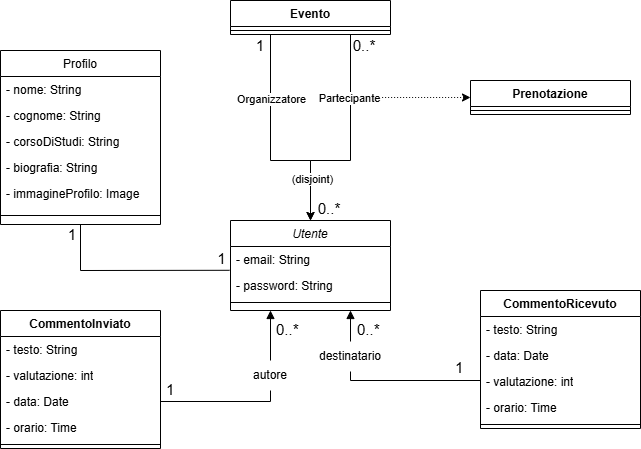
\includegraphics[width=\textwidth,height=0.5\textheight,keepaspectratio]{images/modello-del-dominio-utente.png}
    \caption{Modello del dominio: Utente}
\end{figure}
%
\subsection{Modello del dominio: Evento}
Il modello riguardante l'evento è presentato nel seguente diagramma.

\begin{figure}[H]
    \centering
    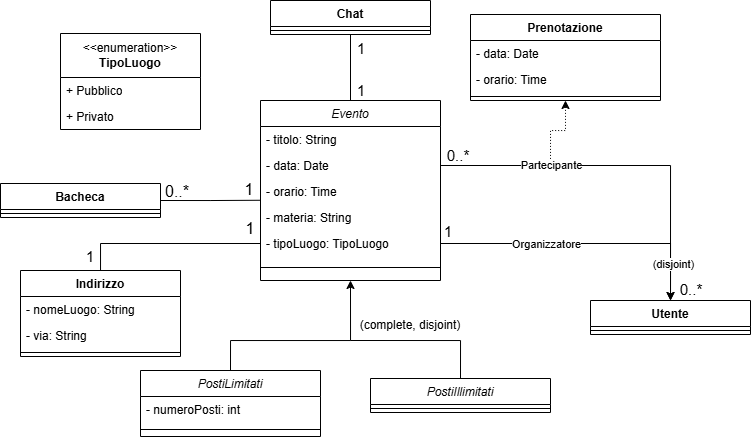
\includegraphics[width=\textwidth,height=0.5\textheight,keepaspectratio]{images/modello-del-dominio-evento.png}
    \caption{Modello del dominio: Evento}
\end{figure}
%
\subsection{Modello del dominio: Filtro}
Il modello riguardante il filtro è presentato nel seguente diagramma.

\begin{figure}[H]
    \centering
    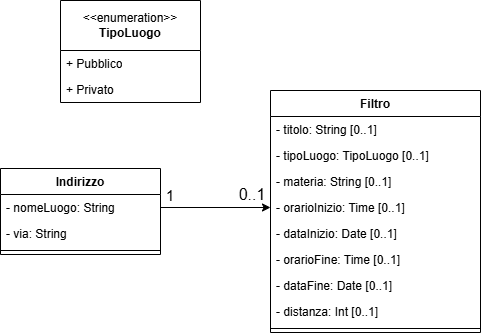
\includegraphics[width=\textwidth,height=0.5\textheight,keepaspectratio]{images/modello-del-dominio-filtro.png}
    \caption{Modello del dominio: Filtro}
\end{figure}
%
\subsection{Modello del dominio: Chat}
Il modello riguardante la chat è presentato nel seguente diagramma.

\begin{figure}[H]
    \centering
    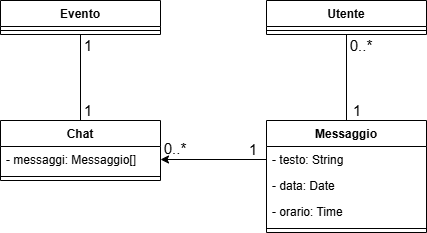
\includegraphics[width=\textwidth,height=0.5\textheight,keepaspectratio]{images/modello-del-dominio-chat.png}
    \caption{Modello del dominio: Chat}
\end{figure}
%
\subsection{Modello del dominio: Log}
Il modello riguardante il log è presentato nel seguente diagramma.

\begin{figure}[H]
    \centering
    
\includegraphics[width=\textwidth,height=0.5\textheight,keepaspectratio]{images/modello-del-dominio-log.png}
    \caption{Modello del dominio: Log}
\end{figure}
%
% Architettura logica
\newpage
\section{Architettura logica}

\subsection{Struttura}

\subsubsection{Diagramma dei package}
Di seguito è presentato il diagramma dei package e le diverse dipendenze che intercorrono tra di loro.

\begin{figure}[H]
    \centering
    
\includegraphics[width=\textwidth,height=0.5\textheight,keepaspectratio]{images/diagramma-dei-package.png}
    \caption{Diagramma dei package}
\end{figure}
%
\subsubsection{Diagramma delle classi: Registrazione e Autenticazione}
Di seguito è presentato il diagramma delle classi di view e controller per la registrazione e autenticazione degli utenti.
Una volta autenticato l'utente è portato alla HomeUtente che è omessa perché connessa semplicemente a tutte le altre home, senza ulteriori funzionalità.

\begin{figure}[H]
    \centering
    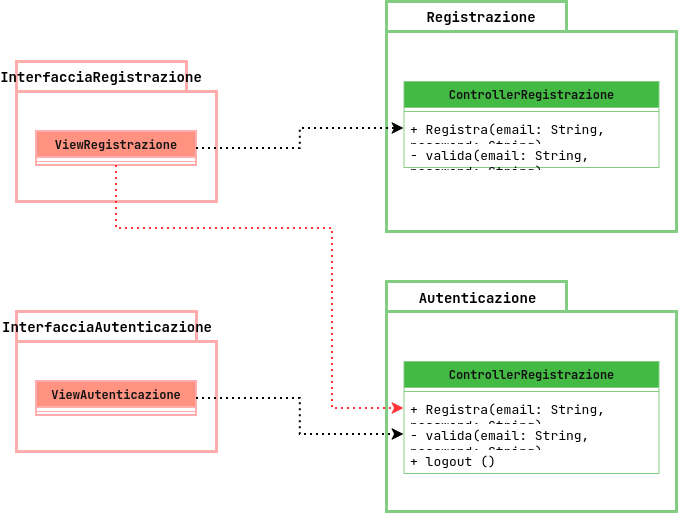
\includegraphics[width=\textwidth,height=0.5\textheight,keepaspectratio]{images/diagramma-dei-package-registrazione-autenticazione.png}
    \caption{Diagramma delle classi: Registrazione e Autenticazione}
\end{figure}
%
\subsubsection{Diagramma delle classi: Profilo}
Di seguito è presentato il diagramma delle classi di view e controller per la gestione del profilo.

\begin{figure}[H]
    \centering
    
\includegraphics[width=\textwidth,height=0.5\textheight,keepaspectratio]{images/diagramma-dei-package-profilo.png}
    \caption{Diagramma delle classi: Profilo}
\end{figure}
%
\subsubsection{Diagramma delle classi: Evento}
Di seguito è presentato il diagramma delle classi di view e controller per la gestione dell'evento.

\begin{figure}[H]
    \centering
    
\includegraphics[width=\textwidth,height=0.5\textheight,keepaspectratio]{images/diagramma-dei-package-evento.png}
    \caption{Diagramma delle classi: Evento}
\end{figure}
%
\subsubsection{Diagramma delle classi: Bacheca}
Di seguito è presentato il diagramma delle classi di view e controller per la gestione della bacheca.

\begin{figure}[H]
    \centering
    
\includegraphics[width=\textwidth,height=0.5\textheight,keepaspectratio]{images/diagramma-dei-package-bacheca.png}
    \caption{Diagramma delle classi: Bacheca}
\end{figure}
%
\subsubsection{Diagramma delle classi: Comunicazione}
Di seguito è presentato il diagramma delle classi di view e controller per la gestione della comunicazione.

\begin{figure}[H]
    \centering
    
\includegraphics[width=\textwidth,height=0.5\textheight,keepaspectratio]{images/diagramma-dei-package-comunicazione.png}
    \caption{Diagramma delle classi: Comunicazione}
\end{figure}
%
\subsection{Interazioni}
Di seguito sono presentate le interazioni tra gli attori e il sistema.

\subsubsection{Interazione: Registrazione}
In figura è presentato un diagramma di sequenza che mostra l'interazione tra i componenti per effettuare la registrazione di un nuovo Utente.

\begin{figure}[H]
    \centering
    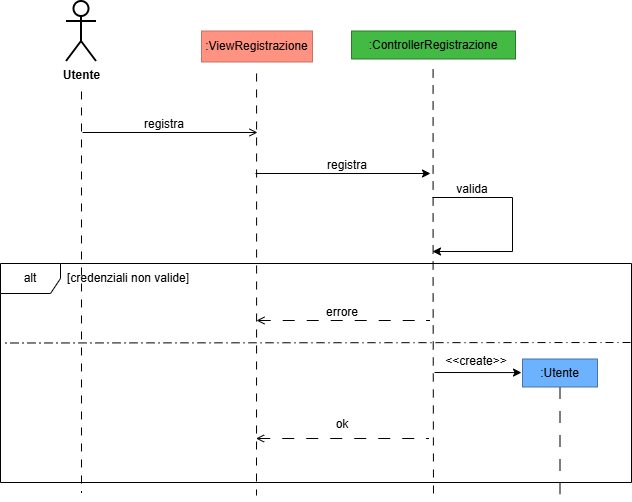
\includegraphics[width=\textwidth,height=0.5\textheight,keepaspectratio]{images/interazione-registrazione.png}
    \caption{Interazione: Registrazione}
\end{figure}
%
\subsubsection{Interazione: Autenticazione}
In figura è presentato un diagramma di sequenza che mostra l'interazione tra i componenti per effettuare l'autenticazione di un Utente esistente.

\begin{figure}[H]
    \centering
    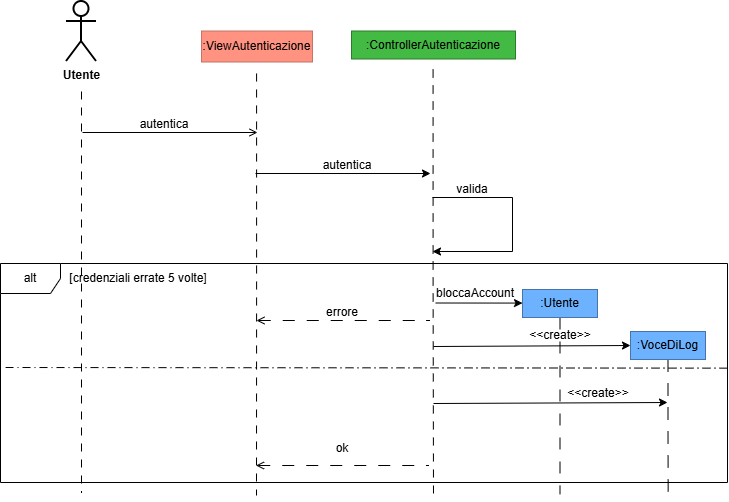
\includegraphics[width=\textwidth,height=0.5\textheight,keepaspectratio]{images/interazione-autenticazione.png}
    \caption{Interazione: Autenticazione}
\end{figure}
%
\subsubsection{Interazione: Elimina Utente}
In figura è presentato un diagramma di sequenza che mostra l'interazione tra i componenti per effettuare l'eliminazione di un Utente esistente.

\begin{figure}[H]
    \centering
    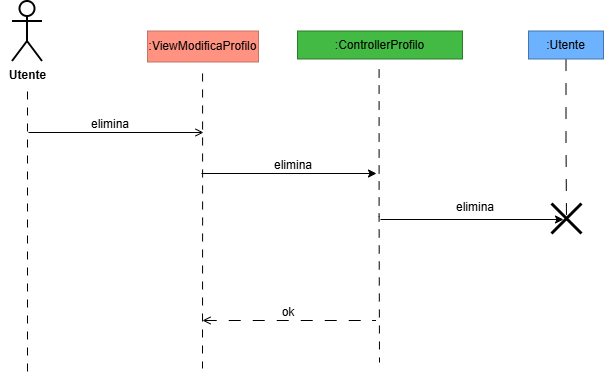
\includegraphics[width=\textwidth,height=0.5\textheight,keepaspectratio]{images/interazione-elimina-utente.png}
    \caption{Interazione: Elimina Utente}
\end{figure}
%
\subsubsection{Interazione: Modifica Profilo}
In figura è presentato un diagramma di sequenza che mostra l'interazione tra i componenti per effettuare la modifica del profilo di un Utente esistente.

\begin{figure}[H]
    \centering
    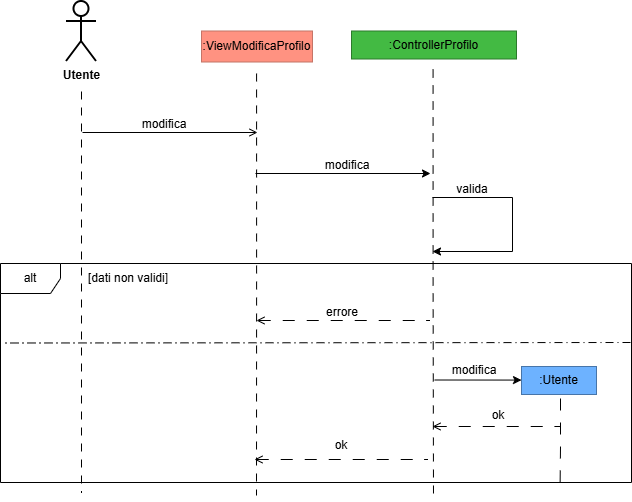
\includegraphics[width=\textwidth,height=0.5\textheight,keepaspectratio]{images/interazione-modifica-profilo.png}
    \caption{Interazione: Modifica Profilo}
\end{figure}
%
\subsubsection{Interazione: Creazione Evento}
In figura è presentato un diagramma di sequenza che mostra l'interazione tra i componenti per effettuare la creazione di un nuovo Evento.

\begin{figure}[H]
    \centering
    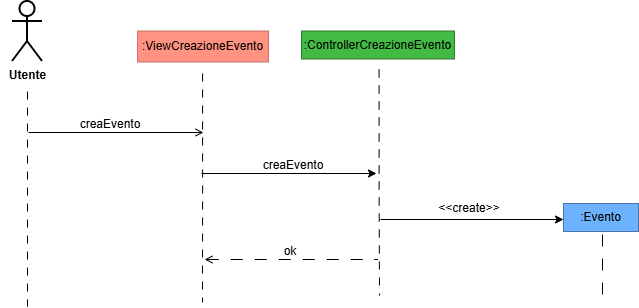
\includegraphics[width=\textwidth,height=0.5\textheight,keepaspectratio]{images/interazione-creazione-evento.png}
    \caption{Interazione: Creazione Evento}
\end{figure}
%
\subsubsection{Interazione: Gestione Evento}
In figura è presentato un diagramma di sequenza che mostra l'interazione tra i componenti per effettuare la gestione di un Evento esistente.

\begin{figure}[H]
    \centering
    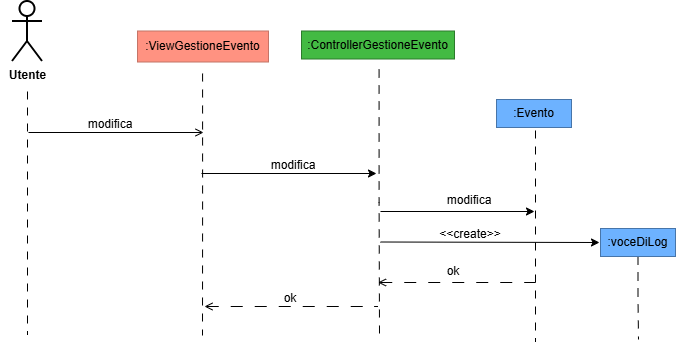
\includegraphics[width=\textwidth,height=0.5\textheight,keepaspectratio]{images/interazione-gestione-evento.png}
    \caption{Interazione: Gestione Evento}
\end{figure}
%
\subsubsection{Interazione: Chat}
In figura è presentato un diagramma di sequenza che mostra l'interazione tra i componenti per effettuare l'utilizzo della Chat.

\begin{figure}[H]
    \centering
    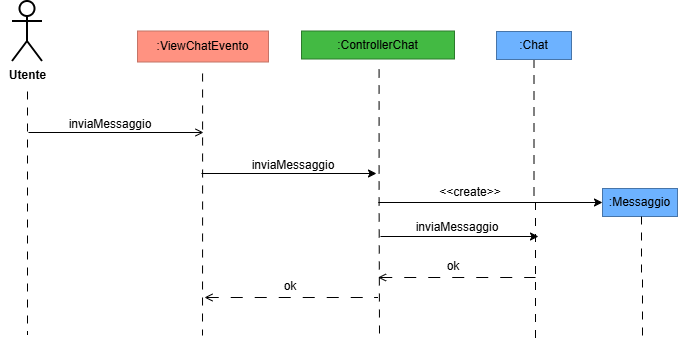
\includegraphics[width=\textwidth,height=0.5\textheight,keepaspectratio]{images/interazione-chat.png}
    \caption{Interazione: Chat}
\end{figure}
%
\subsubsection{Interazione: Commento}
In figura è presentato un diagramma di sequenza che mostra l'interazione tra i componenti per effettuare la creazione di un Commento.

\begin{figure}[H]
    \centering
    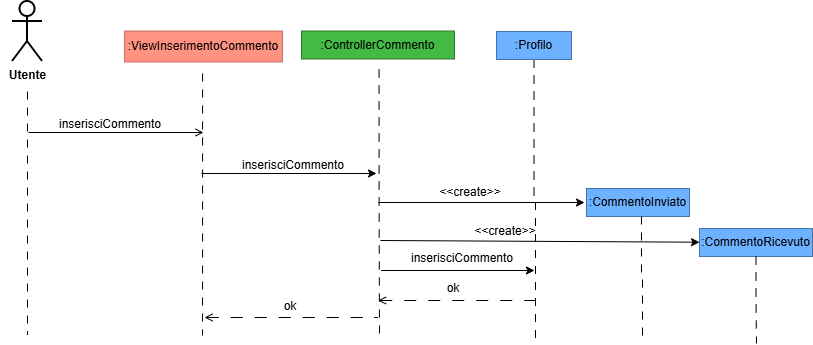
\includegraphics[width=\textwidth,height=0.5\textheight,keepaspectratio]{images/interazione-commento.png}
    \caption{Interazione: Commento}
\end{figure}
%
\subsection{Comportamento}
Dato che il modello non presenta comportamenti particolarmente elaborati, non vengono mostrati i diagrammi di stato.

% Piano di lavoro
\newpage
\section{Piano di lavoro}
\begin{tabularx}{\textwidth}{|X|X|}
    \hline
    \rowcolor{studyColor} \textbf{Nome team} & \textbf{Componenti} \\ \hline
    \endhead
    Team Progettazione & Gattobigio, Lucchi, Porpora \\ \hline
    Team Back-end & Gattobigio, Porpora \\ \hline
    Team Database & Gattobigio, Lucchi, Porpora \\ \hline
    Team Sicurezza & Gattobigio, Lucchi, Porpora \\ \hline
    Team Front-end & Lucchi \\ \hline
\end{tabularx}
\vspace{0.5cm}
\begin{tabularx}{\textwidth}{|X|X|X|}
    \hline
    \rowcolor{studyColor} \textbf{Package} & \textbf{Progetto} & \textbf{Sviluppo} \\ \hline
    \endhead
    InterfacciaRegistrazione & Team Progettazione & Team Front-end \\ \hline
    InterfacciaAutenticazione & Team Progettazione & Team Front-end \\ \hline
    InterfacciaProfilo & Team Progettazione & Team Front-end \\ \hline
    InterfacciaEvento & Team Progettazione & Team Front-end \\ \hline
    InterfacciaBacheca & Team Progettazione & Team Front-end \\ \hline
    InterfacciaComunicazione & Team Progettazione & Team Front-end \\ \hline
    InterfacciaLog & Team Progettazione & Team Front-end \\ \hline
    Registrazione & Team Progettazione & Team Database \\ \hline
    Autenticazione & Team Progettazione & Team Sicurezza \\ \hline
    GestioneProfilo & Team Progettazione & Team Back-end \\ \hline
    GestioneEvento & Team Progettazione & Team Back-end \\ \hline
    GestioneBacheca & Team Progettazione & Team Back-end \\ \hline
    GestioneCommento & Team Progettazione & Team Back-end \\ \hline
    GestioneChat & Team Progettazione & Team Back-end \\ \hline
    Dominio & Team Progettazione & Team Back-end, Team Datebase, Team Sicurezza \\ \hline

\end{tabularx}
\vspace{0.5cm}
\begin{tabularx}{\textwidth}{|X|X|}
    \hline
    \rowcolor{studyColor} \textbf{Periodo} & \textbf{Fase} \\ \hline
    \endhead
    Giugno 2026 & Creazione del primo prototipo. \\ \hline
    Ottobre 2026 & Completamento della prima versione con tutte le funzionalità. \\ \hline
    Dicembre 2026 & Rilascio ad un numero di utenti limitato. \\ \hline
    Febbraio 2027 & Rilascio al pubblico. \\ \hline
\end{tabularx}

\subsection{Caratteristiche primo prototipo (Giugno 2026)}
Il primo prototipo del programma non implementerà tutte le funzionalità previste. Le funzionalità che saranno tralasciate sono in particolare quelle relative al fatto che il programma non sarà rilasciato al pubblico:
\begin{itemize}
    \item La gestione dei log per la sicurezza
    \item La creazione dei termini e le condizioni di utilizzo per adeguarlo al GDPR
    \item Il filtro in base alla distanza dalla posizione dell'Evento, la ricerca è solo possibile tramite corrispondenza delle stringhe dell'indirizzo
\end{itemize}

\subsection{Sviluppi futuri}
Il committente ha richiesto di aggiungere le possibilità di penalizzare gli Utenti a seguito di disiscrizioni a ridosso di Eventi a cui si è iscritti, abbiamo organizzato o comportamenti scorretti.
Inoltre, è stata evidenziata la necessità di introdurre un sistema automatizzato di segnalazione e moderazione dei messaggi e dei commenti, capace di sanzionare o rimuovere autonomamente i contenuti inappropriati.
Si richiede al Team Progettazione di tenere conto di questi sviluppi futuri.

% Piano del collaudo
\newpage
\section{Piano del collaudo}
Di seguito, al fine di non rendere eccessivamente prolissa la trattazione, sono presentati solo alcuni test unitari del sistema.
In particolare, sono stati scelti i test unitari delle classi che si ritengono centrali per il funzionamento del sistema

\subsection{Collaudo: Evento}
\begin{lstlisting}
using NUnit.Framework;

[TestFixture]
public class TestEvento
{
    private Evento eventoLimitato, eventoIllimitato;
    private Profilo organizzatore;
    private Indirizzo indirizzo;

    [SetUp]
    public void Setup()
    {
        organizzatore = new Profilo(
            "Mario", "Rossi",
            "Informatica", "Studente appassionato",
            null
        );

        indirizzo = new Indirizzo("Via Zamboni 33", "Biblioteca Universitaria");

        eventoLimitato = new Evento(
            "Studio Analisi II",
            "Analisi Matematica II",
            new DateTime(2026, 7, 15),
            new Orario("14:00", "17:00"),
            indirizzo,
            TipoDiLuogo.Pubblico,
            5,
            organizzatore
        );

        eventoIllimitato = new Evento(
            "Ripasso Algebra",
            "Algebra e Geometria",
            new DateTime(2026, 7, 20),
            new Orario("10:00", "13:00"),
            indirizzo,
            TipoDiLuogo.Privato,
            0,
            organizzatore
        );
    }

    [Test]
    public void TestCreazioneEvento()
    {
        Assert.AreEqual("Studio Analisi II",
            eventoLimitato.getTitolo());
        Assert.AreEqual("Analisi Matematica II",
            eventoLimitato.getMateria());
        Assert.AreEqual(new DateTime(2026, 7, 15),
            eventoLimitato.getData());
        Assert.AreEqual(new Orario("14:00", "17:00"),
            eventoLimitato.getOrario());
        Assert.AreEqual(indirizzo,
            eventoLimitato.getIndirizzo());
        Assert.AreEqual(TipoDiLuogo.Pubblico,
            eventoLimitato.getTipoDiLuogo());
        Assert.AreEqual(5,
            eventoLimitato.getNumeroPosti());
        Assert.AreEqual(organizzatore,
            eventoLimitato.getOrganizzatore());
    }

    [Test]
    public void TestEventoIllimitato()
    {
        Assert.AreEqual("Ripasso Algebra",
            eventoIllimitato.getTitolo());
        Assert.AreEqual(TipoDiLuogo.Privato,
            eventoIllimitato.getTipoDiLuogo());
        Assert.AreEqual(0,
            eventoIllimitato.getNumeroPosti());
    }

    [Test]
    public void TestPartecipanti()
    {
        Profilo partecipante = new Profilo(
            "Luca", "Bianchi",
            "Informatica", "Studio volentieri in gruppo",
            null
        );
        eventoLimitato.aggiungiPartecipante(partecipante);

        CollectionAssert.Contains(
            eventoLimitato.getPartecipanti(),
            partecipante
        );
        Assert.AreEqual(1,
            eventoLimitato.getPartecipanti().Count);
    }

    [Test]
    public void TestRimozionePartecipante()
    {
        Profilo partecipante = new Profilo(
            "Luca", "Bianchi",
            "Informatica", "Studio volentieri in gruppo",
            null
        );
        eventoLimitato.aggiungiPartecipante(partecipante);
        eventoLimitato.rimuoviPartecipante(partecipante);

        CollectionAssert.DoesNotContain(
            eventoLimitato.getPartecipanti(),
            partecipante
        );
        Assert.AreEqual(0,
            eventoLimitato.getPartecipanti().Count);
    }

    [Test]
    public void TestPostiDisponibili()
    {
        Assert.AreEqual(5,
            eventoLimitato.getPostiDisponibili());

        Profilo partecipante = new Profilo(
            "Luca", "Bianchi",
            "Informatica", "Studio volentieri in gruppo",
            null
        );
        eventoLimitato.aggiungiPartecipante(partecipante);

        Assert.AreEqual(4,
            eventoLimitato.getPostiDisponibili());
    }

    [Test]
    public void TestChatGenerata()
    {
        Assert.IsNotNull(eventoLimitato.getChat());
    }
}
\end{lstlisting}

\subsection{Collaudo: Profilo}
\begin{lstlisting}
using NUnit.Framework;

[TestFixture]
public class TestProfilo
{
    private Profilo profiloCompleto, profiloMinimo;

    [SetUp]
    public void Setup()
    {
        profiloCompleto = new Profilo(
            "Mario", "Rossi",
            "Ingegneria Informatica",
            "Studente del terzo anno",
            "immagine.png"
        );

        profiloMinimo = new Profilo(
            "Luca", "Bianchi",
            "Matematica",
            "",
            null
        );
    }

    [Test]
    public void TestCreazioneProfilo()
    {
        Assert.AreEqual("Mario",
            profiloCompleto.getNome());
        Assert.AreEqual("Rossi",
            profiloCompleto.getCognome());
        Assert.AreEqual("Ingegneria Informatica",
            profiloCompleto.getCorsoDiStudi());
        Assert.AreEqual("Studente del terzo anno",
            profiloCompleto.getBiografia());
        Assert.AreEqual("immagine.png",
            profiloCompleto.getImmagine());
    }

    [Test]
    public void TestProfiloMinimo()
    {
        Assert.AreEqual("Luca",
            profiloMinimo.getNome());
        Assert.AreEqual("Bianchi",
            profiloMinimo.getCognome());
        Assert.AreEqual("Matematica",
            profiloMinimo.getCorsoDiStudi());
        Assert.AreEqual("",
            profiloMinimo.getBiografia());
        Assert.IsNull(profiloMinimo.getImmagine());
    }

    [Test]
    public void TestSetterProfilo()
    {
        profiloCompleto.setNome("Giuseppe");
        Assert.AreEqual("Giuseppe",
            profiloCompleto.getNome());

        profiloCompleto.setCognome("Verdi");
        Assert.AreEqual("Verdi",
            profiloCompleto.getCognome());

        profiloCompleto.setCorsoDiStudi("Fisica");
        Assert.AreEqual("Fisica",
            profiloCompleto.getCorsoDiStudi());

        profiloCompleto.setBiografia("Nuova biografia");
        Assert.AreEqual("Nuova biografia",
            profiloCompleto.getBiografia());

        profiloCompleto.setImmagine("nuova_immagine.png");
        Assert.AreEqual("nuova_immagine.png",
            profiloCompleto.getImmagine());
    }

    [Test]
    public void TestCommenti()
    {
        Commento commento = new Commento(
            profiloMinimo,
            "Ottimo compagno di studio",
            4,
            new DateTime(2026, 7, 16),
            new Orario("18:00")
        );
        profiloCompleto.aggiungiCommento(commento);
        CollectionAssert.Contains(
            profiloCompleto.getCommenti(),
            commento
        );
        Assert.AreEqual(1,
            profiloCompleto.getCommenti().Count);
    }
}
\end{lstlisting}

% Progettazione
\newpage
\chapter{Progettazione}

% Progettazione architetturale
\section{Progettazione architetturale}

\subsection{Requisiti non funzionali}
Dall'Analisi del Problema (Tabella Vincoli) sono emersi diversi requisiti non funzionali che impongono dei vincoli al sistema, in particolare l'usabilità (accessibilità e reattività) e la sicurezza (protezione dei dati personali). 

Questi due aspetti si trovano parzialmente in contrasto tra loro, poiché misure di sicurezza molto stringenti possono peggiorare l'esperienza d'uso e rallentare i tempi di risposta. Per gestire questo problema e bilanciare i requisiti, sono state prese le seguenti decisioni:
\begin{itemize}
    \item \textbf{Sicurezza}: si è scelto di utilizzare protocolli crittografici standard per la protezione dei canali di comunicazione pubblici e meccanismi robusti per il controllo degli accessi e la gestione delle sessioni (tramite token).
    \item \textbf{Usabilità e Portabilità}: per favorire l'uso dell'applicazione da molteplici dispositivi, si è deciso di salvare i dati in modo centralizzato su un database remoto e non in locale sul dispositivo dell'utente, esponendo i servizi tramite API fruibili via web.
\end{itemize}

\subsection{Scelta dell'architettura}
Dal punto di vista architetturale, per rispettare i requisiti evidenziati, l'architettura più idonea per il sistema è un'architettura Client/Server Web a 3 livelli:

\begin{itemize}
    \item \textbf{L1 - Client}: Il client si occupa della presentazione e dell'interazione con l'utente. Per garantire un'elevata reattività dell'interfaccia, specialmente per funzionalità che richiedono aggiornamenti dinamici come la Chat di gruppo, si opta per un approccio basato su \textit{fat client} (Single Page Application). In questo modo il client delega le elaborazioni complesse al server e gestisce lo stato dell'interfaccia.
    \item \textbf{L2 - Server}: Il server si occupa di accentrare la logica di business, il controllo degli accessi e la validazione dei dati. Il server metterà a disposizione delle API REST (\textit{Representational State Transfer}) \textit{stateless} per la gestione standard dell'applicativo. Inoltre, per gestire le funzionalità in tempo reale come la Chat di gruppo, il server gestirà connessioni persistenti e bidirezionali tramite protocollo WebSocket. L'utilizzo di API stateless unito a WebSocket permette di coniugare scalabilità e reattività.
    \item \label{L3-Persistenza}\textbf{L3 - Persistenza}: Per la gestione della persistenza si avrà un server dedicato nel quale sarà installato un opportuno DBMS che gestirà in modo completo la base dati dell'applicazione. Per risolvere il conflitto di impedenza tra il modello a oggetti del server e il modello relazionale del database, verrà utilizzato il paradigma Object-Relational Mapping (ORM).
\end{itemize}

\subsection{Scelte tecnologiche}
Al fine di favorire la separazione delle responsabilità e la manutenibilità del codice, si è scelto di adottare il pattern architetturale Model-View-Controller (MVC) sul lato server e Model-View-ViewModel (MVVM) sul lato frontend.

Per la comunicazione tra L1 e L2 verrà utilizzato il protocollo HTTPS, in modo che il livello TLS garantisca l'integrità e la riservatezza dei dati scambiati, tutelando la privacy degli utenti. Le richieste alle API saranno autenticate tramite l'uso di token di sessione sicuri (es. JSON Web Token).

In aggiunta alle API REST, data l'importanza del requisito della Chat di gruppo per gli Eventi di studio, il server adotterà tecnologie capaci di mantenere una comunicazione bidirezionale in tempo reale (come il protocollo WebSocket), permettendo ai client di ricevere e inviare i nuovi messaggi con latenza minima.


Per il Client (L1), verrà impiegato un framework web frontend reattivo moderno (React), utilizzando lo strumento di build \textit{Vite} per velocizzare l'ambiente di sviluppo locale e ottimizzare la compilazione finale dei file statici.
Per l'implementazione del Server (L2), si utilizzerà un framework web lato server robusto, orientato agli oggetti e ad alte prestazioni (es. ASP.NET con C\#).
Per la Persistenza (L3), la scelta ricade su un DBMS relazionale (PostgreSQL), adatto alla natura strutturata dei dati del dominio, interfacciato tramite la libreria ORM nativa.

\subsection{Diagramma dei package}
Di seguito è riportato il diagramma dei package dell'applicazione.
La presenza di un layer di persistenza (viola) tra i controller e il modello permette una certa trasparenza rispetto alle operazioni di salvataggio e lettura dei dati nel livello dei controller.
Si sceglie di utilizzare la tecnica ORM (come spiegato in \hyperref[L3-Persistenza]{L3 - Persistenza}) per mappare le entità alle tabelle del database.

\begin{figure}[H]
    \centering
    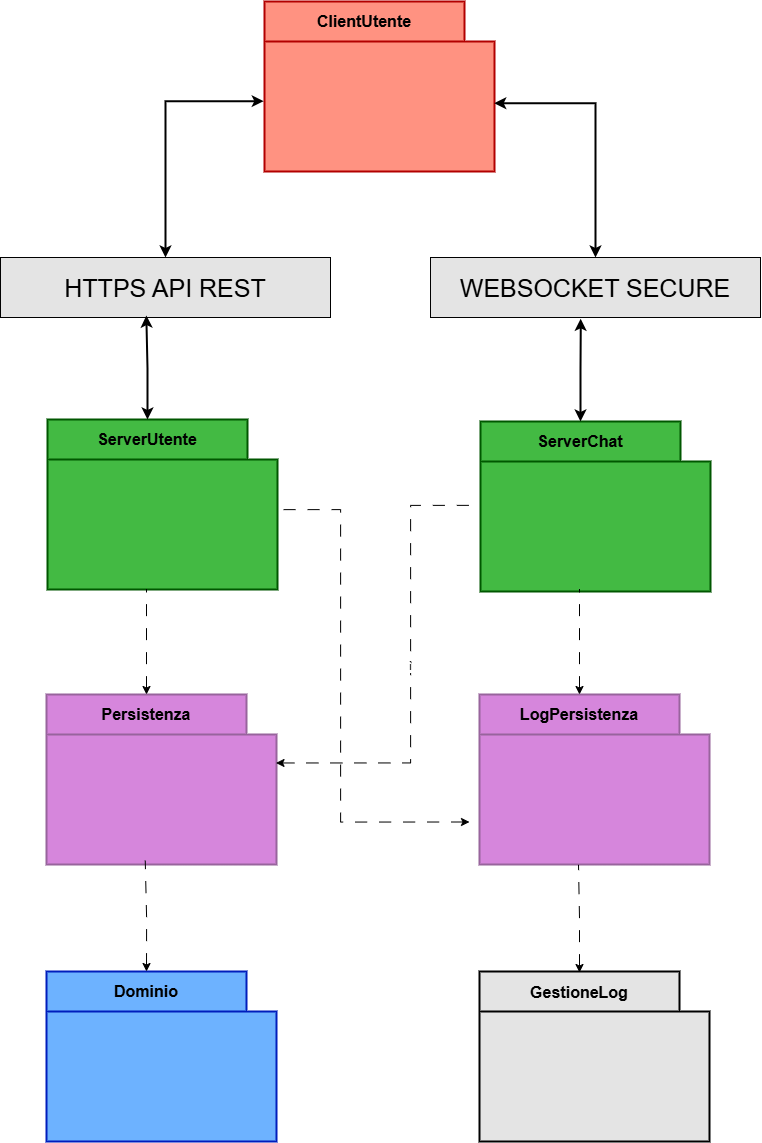
\includegraphics[width=\textwidth,height=0.5\textheight,keepaspectratio]{images/diagramma-dei-package-progettazione.png}
    \caption{Diagramma dei package: Progettazione}
\end{figure}
%
\subsection{Diagramma dei componenti}
Nella figura sottostante è riportata l'architettura del Sistema, organizzata attraverso un diagramma del componenti.

\begin{figure}[H]
    \centering
    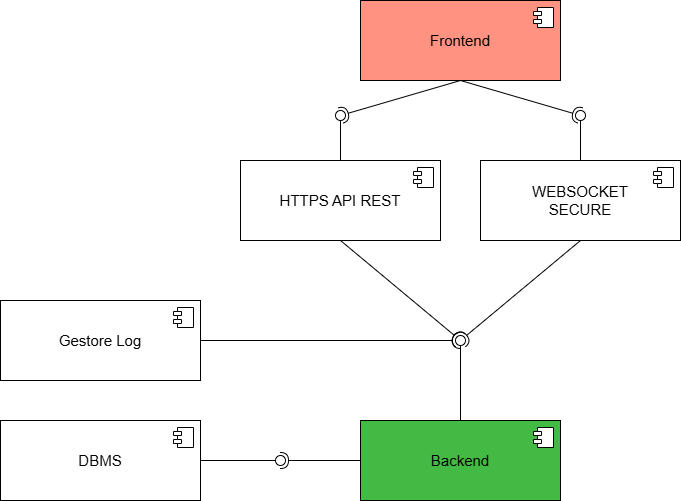
\includegraphics[width=\textwidth,height=0.5\textheight,keepaspectratio]{images/diagramma-dei-componenti-progettazione.png}
    \caption{Diagramma dei componenti}
\end{figure}
%
% Progettazione di dettaglio
\newpage
\section{Progettazione di dettaglio}

\subsection{Struttura}

\subsubsection{Diagrammi di dettaglio del modello}

\paragraph{Diagramma di dettaglio: Account}

Di seguito è presentato il diagramma delle classi del modello del dominio riguardante l'Account.

\begin{figure}[H]
    \centering
    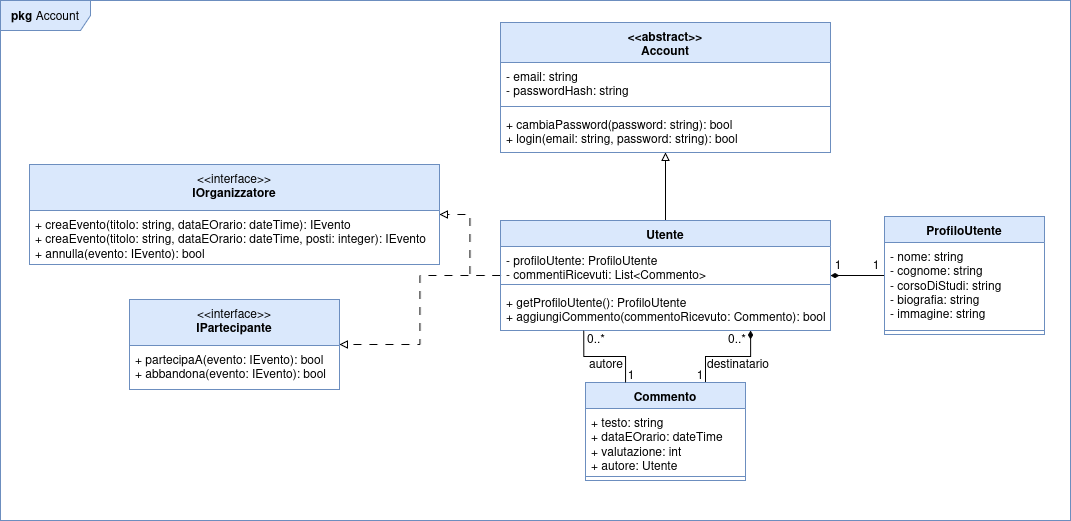
\includegraphics[width=\textwidth,height=0.5\textheight,keepaspectratio]{images/diagramma-di-dettaglio-account.png}
    \caption{Diagramma di dettaglio: Account}
\end{figure}
%
In questo diagramma è da notare che:
\begin{itemize}[leftmargin=*]
    \item Il concetto generale di fruitore del sistema è stato rinominato da Utente ad Account per favorire l'espandibilità dell'applicazione.
    \item È stata introdotta la classe astratta Account, la quale incapsula esclusivamente i dati fondamentali di base (come l'email), mentre le informazioni sensibili di autenticazione (come l'hash della password) sono gestite direttamente dal database tramite il contesto.
    \item La sottoclasse Utente modella lo studente standard che utilizza l'app, raggruppando i dettagli del ProfiloUtente e la lista dei commentiRicevuti. Questa separazione permette l'introduzione futura di nuovi account istituzionali (come ad esempio un account gestito direttamente da UniBo per promuovere sessioni di studio) che non necessitano di campi incompatibili, come il corso di studi o il sistema di recensioni tramite commenti.
    \item Per favorire il disaccoppiamento e rispettare il principio di segregazione delle interfacce (ISP), sono state create le interfacce IOrganizzatore e IPartecipante. In questo modo, eventuali enti organizzatori futuri potranno implementare solo la logica di creazione degli eventi, senza essere forzati ad implementare la logica di partecipazione, tipica invece delle persone fisiche.
    \item Rispetto all'analisi, in cui erano presenti due entità separate (\texttt{CommentoInviato} e \texttt{CommentoRicevuto}), si è scelto di unificare la struttura in una singola classe \texttt{Commento}. Questa contiene gli attributi comuni (testo, valutazione, data e orario) ed esprime il mittente e il destinatario attraverso due relazioni distinte con l'entità \texttt{Utente}. Tale approccio riduce la duplicazione del codice, semplifica la logica di business e agevola la persistenza dei dati sul database, mantenendo al contempo una chiara tracciabilità bidirezionale.
    \item A livello di modello logico, per l'Account sono stati previsti attributi come \texttt{tentativiFalliti} e \texttt{scadenzaBlocco} per gestire la sicurezza dell'accesso: dopo 5 errori di autenticazione consecutivi, l'account viene sospeso temporaneamente.
\end{itemize}

\newpage
\paragraph{Diagramma di dettaglio: Evento}

Di seguito è presentato il diagramma delle classi del modello del dominio riguardante gli Eventi.

\begin{figure}[H]
    \centering
    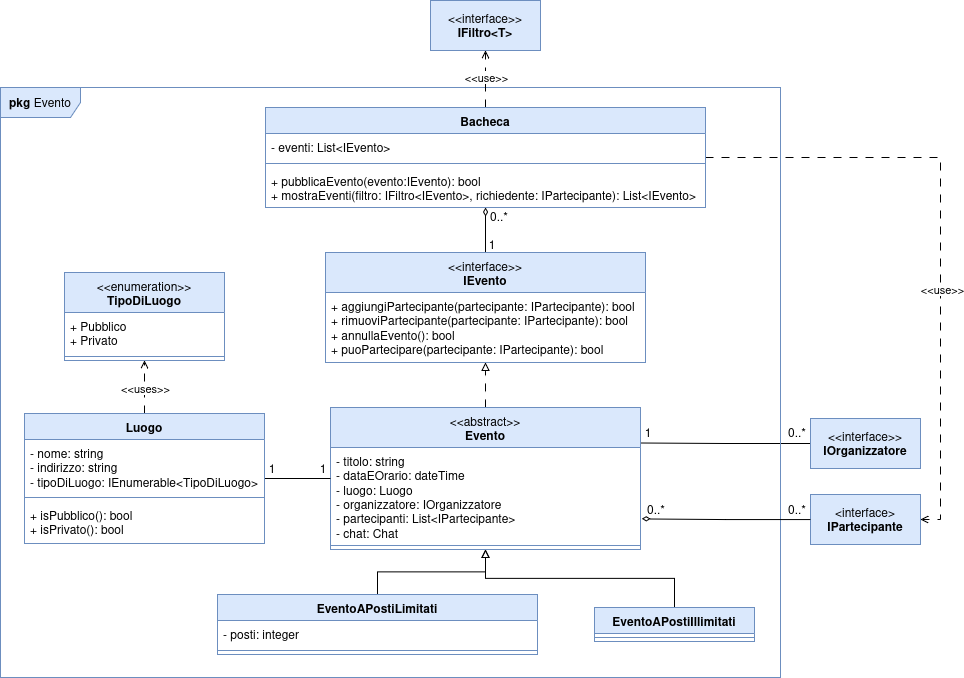
\includegraphics[width=\textwidth,height=0.5\textheight,keepaspectratio]{images/diagramma-di-dettaglio-evento.png}
    \caption{Diagramma di dettaglio: Evento}
\end{figure}
%
In questo diagramma è da notare che:
\begin{itemize}[leftmargin=*]
    \item È stata definita l'interfaccia IEvento che impone i metodi contrattuali di base (aggiungiPartecipante, rimuoviPartecipante, annullaEvento, puoPartecipare). Questo garantisce un alto grado di espandibilità (Open/Closed Principle): se in futuro si volessero modellare nuove tipologie di attività, come ad esempio sessioni di studio telematiche (che necessitano di un link anziché di un Indirizzo fisico) o eventi come esami o conferenze, queste potranno implementare l'interfaccia senza alterare la logica preesistente del sistema.
    \item Rispetto alla fase di analisi in cui la capienza era un semplice parametro, la classe astratta \texttt{Evento} si specializza nelle classi concrete \texttt{EventoAPostiLimitati} (che introduce l'attributo privato \texttt{posti}) ed \texttt{EventoAPostiIllimitati}. Questa scelta garantisce scalabilità ed estensibilità: le logiche di validazione delle iscrizioni e il calcolo dei posti disponibili sono delegate, evitando l'uso di complessi blocchi condizionali nel codice client e facilitando l'eventuale introduzione futura di eventi con logiche di accesso differenti.
    \item È stata introdotta la classe Bacheca per centralizzare la gestione e l'accesso agli eventi. Essa funge da punto di raccolta unico e fornisce i metodi utili alla pubblicazione e al filtraggio degli eventi per l'interfaccia utente.
    \item L'introduzione dell'enumerazione TipoDiLuogo permette di limitare e tipizzare in modo sicuro la definizione di un luogo, specificando chiaramente se esso è pubblico o privato.
\end{itemize}

\newpage
\paragraph{Diagramma di dettaglio: Chat}

Di seguito è presentato il diagramma delle classi del modello del dominio riguardante la Chat.

\begin{figure}[H]
    \centering
    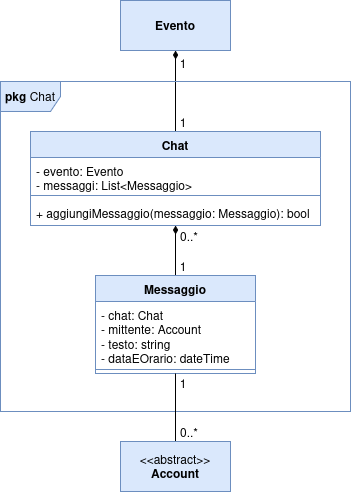
\includegraphics[width=\textwidth,height=0.5\textheight,keepaspectratio]{images/diagramma-di-dettaglio-chat.png}
    \caption{Diagramma di dettaglio: Chat}
\end{figure}
%
In questo diagramma è da notare che:
\begin{itemize}[leftmargin=*]
    \item La struttura è stata progettata per essere estremamente lineare e focalizzata. La classe Chat modella l'insieme della conversazione fungendo da aggregatore per la lista di messaggi.
    \item La cardinalità definisce in modo stringente che una Chat appartiene ad uno e un solo Evento.
    \item La classe Messaggio incapsula tutte le informazioni necessarie per la tracciabilità delle comunicazioni, mantenendo al suo interno i riferimenti alla Chat di appartenenza, all'Account del mittente, il contenuto testuale e il timestamp temporale (dataEOrario).
\end{itemize}

\newpage
\paragraph{Diagramma di dettaglio: Filtro}

Di seguito è presentato il diagramma delle classi del modello del dominio riguardante i Filtri.

\begin{figure}[H]
    \centering
    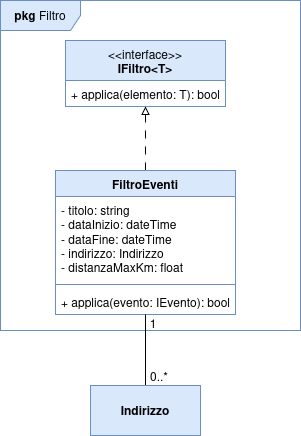
\includegraphics[width=\textwidth,height=0.5\textheight,keepaspectratio]{images/diagramma-di-dettaglio-filtro.png}
    \caption{Diagramma di dettaglio: Filtro}
\end{figure}
%
In questo diagramma è da notare che:
\begin{itemize}[leftmargin=*]
    \item È stata creata l'interfaccia generica \texttt{IFiltro<T>} dotata del metodo applica(). Questa scelta architetturale applica il pattern Strategy e garantisce il pieno rispetto del principio Open/Closed (OCP), permettendo di aggiungere agilmente in futuro nuovi criteri di filtraggio senza dover modificare il codice delle classi client (come la Bacheca).
    \item La classe FiltroEventi raggruppa logicamente tutti i molteplici parametri di ricerca (come titolo, finestre temporali, indirizzo e distanzaMaxKm), evitando così lunghe liste di parametri nei metodi e migliorando la coesione dei dati di ricerca.
    \item Il filtro basato su \texttt{distanzaMaxKm} calcola la distanza fisica (in chilometri) tra due punti geografici distinti: l'indirizzo inserito in input dall'utente (che fa da centro) e l'indirizzo dell'evento. Entrambi gli indirizzi stradali vengono geocodificati in coordinate di latitudine e longitudine; dopodiché, la distanza tra i due punti viene calcolata geometricamente sulla superficie terrestre, includendo nella bacheca del client solo gli eventi che ricadono nel raggio impostato.
\end{itemize}

\newpage
\paragraph{Diagramma di dettaglio: Log}

Di seguito è presentato il diagramma delle classi del modello del dominio riguardante i Log.

\begin{figure}[H]
    \centering
    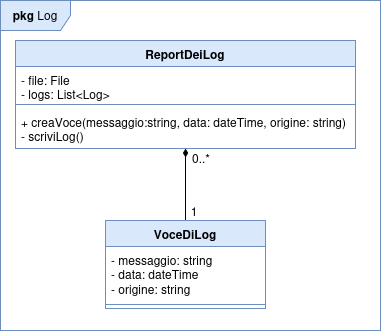
\includegraphics[width=0.5\textwidth,height=0.5\textheight,keepaspectratio]{images/diagramma-di-dettaglio-log.png}
    \caption{Diagramma di dettaglio: Log}
\end{figure}
%
In questo diagramma è da notare che:
\begin{itemize}[leftmargin=*]
    \item Nel rispetto del principio di singola responsabilità (SRP), l'intera gestione del tracciamento è stata isolata all'interno della classe ReportDeiLog, che si occupa di aggregare le singole entità VoceDiLog e gestire il file di output.
    \item Il metodo scriviLog() all'interno di ReportDeiLog è stato reso privato: esso è progettato per essere invocato periodicamente e in background da un Thread separato. Questo approccio permette di riversare sul file di testo le VoceDiLog generate nell'ultimo periodo senza bloccare o rallentare il flusso di esecuzione principale dell'applicazione.
\end{itemize}


\newpage
\subsubsection{Diagramma di dettaglio: Client}

\paragraph{Client: Interfaccia Profilo}
Di seguito è presentato il diagramma delle classi dell'interfaccia del profilo.

\begin{figure}[H]
    \centering
    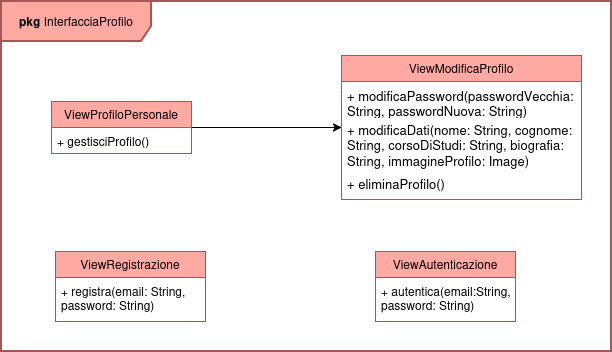
\includegraphics[width=\textwidth,height=0.5\textheight,keepaspectratio]{images/diagramma-di-dettaglio-interfaccia-profilo.png}
    \caption{Diagramma di dettaglio: Interfaccia Profilo}
\end{figure}
%
É da notare che rispetto all'analisi si è scelto di separare il metodo \texttt{modificaProfilo()} nei metodi \texttt{modificaDati()} e \texttt{modificaPassword()}.

\paragraph{Client: Interfaccia Evento}
Di seguito è presentato il diagramma delle classi dell'interfaccia dell'evento.

\begin{figure}[H]
    \centering
    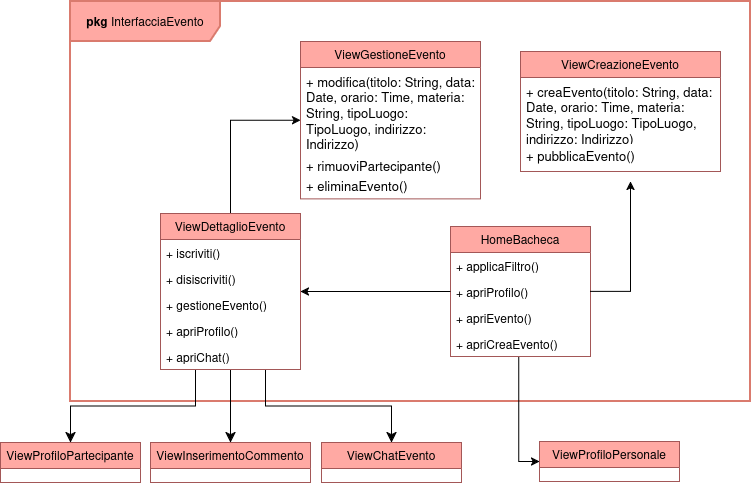
\includegraphics[width=\textwidth,height=0.5\textheight,keepaspectratio]{images/diagramma-di-dettaglio-interfaccia-evento.png}
    \caption{Diagramma di dettaglio: Interfaccia Evento}
\end{figure}
%
\paragraph{Client: Interfaccia Comunicazione}
Di seguito è presentato il diagramma delle classi dell'interfaccia della comunicazione.

\begin{figure}[H]
    \centering
    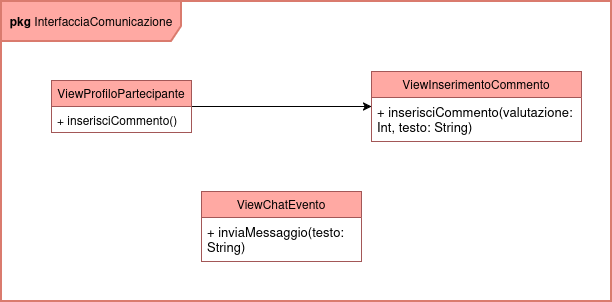
\includegraphics[width=\textwidth,height=0.5\textheight,keepaspectratio]{images/diagramma-di-dettaglio-interfaccia-comunicazione.png}
    \caption{Diagramma di dettaglio: Interfaccia Comunicazione}
\end{figure}
%
\newpage
\subsubsection{Diagramma di dettaglio: Controller}

Di seguito sono presentati i diagrammi di dettaglio relativi ai Controller dell'applicazione. Come spiegato nella scelta dell'architettura e nelle scelte tecnologiche, è stato deciso di mettere a disposizione delle API REST per permettere l'interazione tra client e server. A questo fine, è da considerare che:
\begin{itemize}[leftmargin=*]
    \item Per migliorare l'interoperabilità e renderlo più manutenibile, si è scelto di utilizzare i DTO (Data Transfer Object) in modo da non esporre direttamente il dominio. Dato che generalmente rispettano la struttura delle classi già mostrate, in questo documento si ignoreranno.
    \item Per rendere più efficiente e sostenibile la comunicazione, si è scelto di utilizzare la paginazione quando si richiedono liste di oggetti, in modo da non sovraccaricare il server e il client con dati inutili. Tuttavia, per semplificare la lettura dei diagrammi, non si è rappresentata la paginazione.
    \item Per gestire l'autorizzazione e l'autenticazione, si è scelto di utilizzare i token JWT (JSON Web Token) che permettono di identificare l'utente e le sue autorizzazioni. Per semplificare la lettura dei diagrammi, la loro gestione non è stata rappresentata.
\end{itemize}


\paragraph{Server: Interfacce}
\begin{figure}[H]
    \centering
    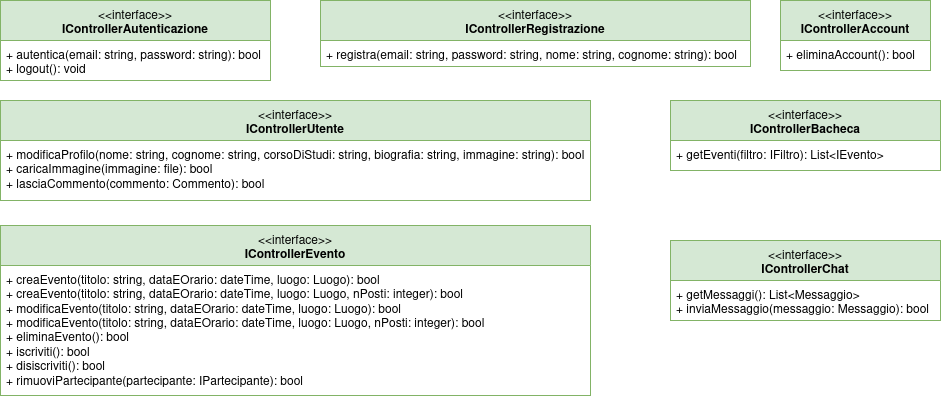
\includegraphics[width=\textwidth,height=0.5\textheight,keepaspectratio]{images/diagramma-di-dettaglio-interfacce-controller.png}
    \caption{Diagramma di dettaglio: Interfacce Controller}
\end{figure}
%

\paragraph{Server: Controller}

Di seguito è presentato il diagramma di dettaglio delle implementazioni dei controller.

\begin{figure}[H]
    \centering
    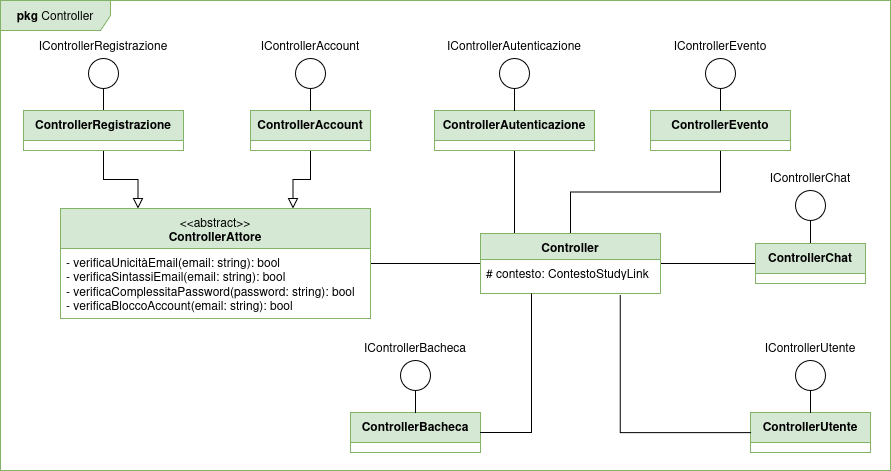
\includegraphics[width=\textwidth,height=0.5\textheight,keepaspectratio]{images/diagramma-di-dettaglio-implementazione-controller.png}
    \caption{Diagramma di dettaglio: Implementazione Controller}
\end{figure}
%
È da notare che:
\begin{itemize}[leftmargin=*]
    \item Tutti i controller condividono una classe base comune \texttt{Controller}, la quale detiene il riferimento protetto al contesto del database (\texttt{\# contesto: ContestoStudyLink}). In questo modo, l'accesso alle tabelle tramite ORM è centralizzato ed ereditato in modo uniforme.
    \item È stata introdotta la classe astratta \texttt{ControllerAttore} (che estende la classe base \texttt{Controller}) come superclasse per \texttt{ControllerRegistrazione} e \texttt{ControllerAccount}, centralizzando le logiche di validazione legate all'anagrafica degli attori.
    \item All'interno di \texttt{ControllerAttore} sono definiti esclusivamente come privati (\texttt{-}) i metodi di validazione sensibili: \texttt{verificaUnicitàEmail()}, \texttt{verificaSintassiEmail()} e \texttt{verificaComplessitàPassword()}. Questa soluzione assicura che tali metodi critici non siano accessibili o invocabili dall'esterno dell'architettura dei controller, garantendo una maggiore sicurezza ed evitando la duplicazione di codice.
    \item Ogni controller concreto implementa la sua rispettiva interfaccia (come ad esempio \texttt{IControllerRegistrazione} e \texttt{IControllerAccount}), garantendo il disaccoppiamento tra la definizione delle API del server e la loro effettiva implementazione.
    \item All'interno del controller preposto all'autenticazione è implementata la logica per il blocco temporaneo dell'account in caso di molteplici errori. Durante il login, il controller verifica i \texttt{tentativiFalliti}: se raggiungono o superano quota 5, il sistema rifiuta l'accesso a prescindere dalla validità delle credenziali inserite e imposta la \texttt{scadenzaBlocco} per inibire ulteriori tentativi per 15 minuti.
\end{itemize}

\newpage
\subsubsection{Diagramma di dettaglio: Persistenza}

\paragraph{Persistenza: ContestoStudyLink}
La classe ContestoStudyLink è utilizzata dall'ORM per interfacciarsi con il DBMS.

\begin{figure}[H]
    \centering
    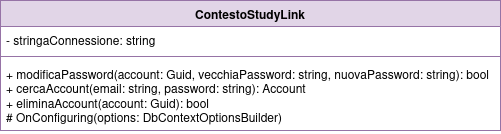
\includegraphics[width=0.5\textwidth,height=0.5\textheight,keepaspectratio]{images/diagramma-di-dettaglio-persistenza.png}
    \caption{Diagramma di dettaglio: Persistenza}
\end{figure}
%

\subsection{Interazioni}
Di seguito sono presentate le figure che mostrano le interazioni tra i componenti per le principali funzionalità del sistema.

\subsubsection{Interazione: Autenticazione}
Di seguito è presentata la figura che mostra le interazioni tra i componenti per l'autenticazione dell'utente.

\begin{figure}[H]
    \centering
    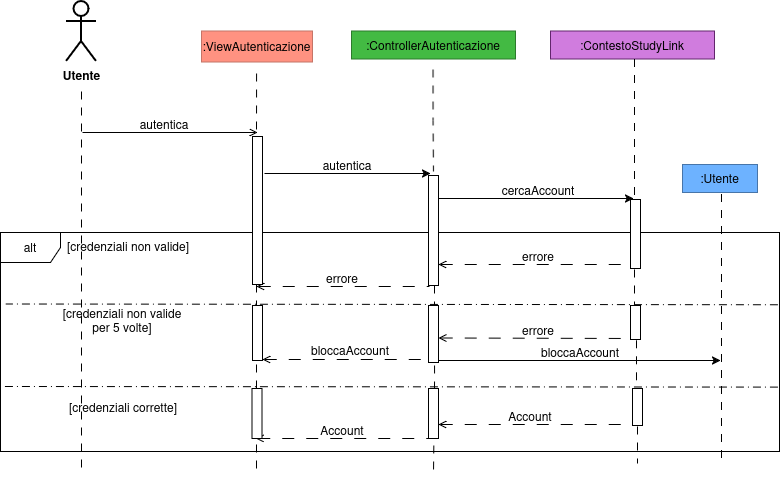
\includegraphics[width=\textwidth,height=0.5\textheight,keepaspectratio]{images/interazione-progettazione-autenticazione.png}
    \caption{Diagramma di sequenza: Autenticazione}
\end{figure}
%
\subsubsection{Interazione: Gestione profilo}
Di seguito sono presentate le figure che mostrano le interazioni tra i componenti per la gestione del profilo dell'utente.

\begin{figure}[H]
    \centering
    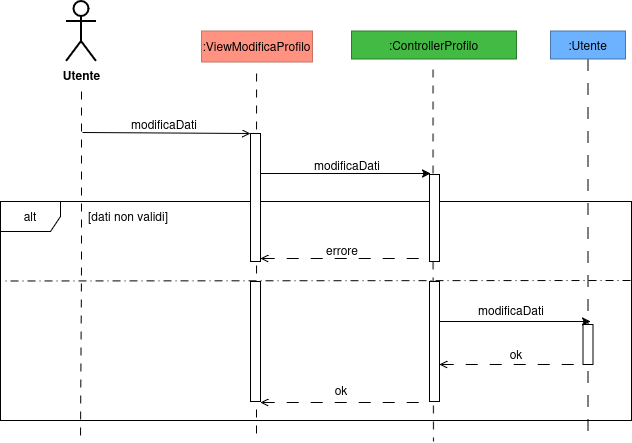
\includegraphics[width=\textwidth,height=0.5\textheight,keepaspectratio]{images/interazione-progettazione-modifica-dati.png}
    \caption{Diagramma di sequenza: Gestione profilo - Modifica dati}
\end{figure}
%
Il metodo che in analisi è \texttt{modificaProfilo()} è stato diviso in \texttt{modificaDati()} e \texttt{modificaPassword()} per poter applicare controlli diversi a seconda dell'importanza dei dati.
Anche se non è indicato nel diagramma, per motivi di spazio, ci sarà la memorizzazione dei dati sul database e la scrittura dei log.

\begin{figure}[H]
    \centering
    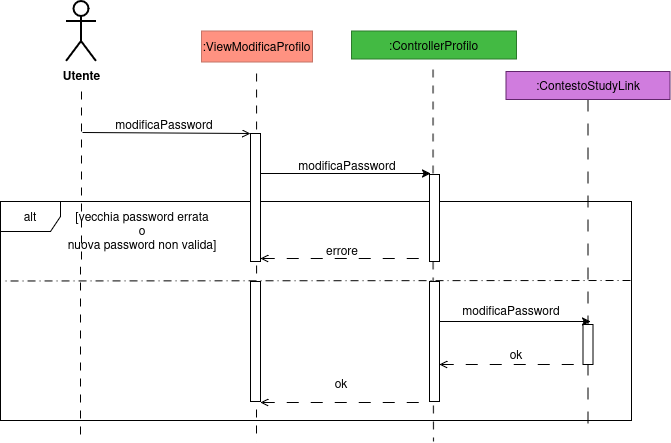
\includegraphics[width=\textwidth,height=0.5\textheight,keepaspectratio]{images/interazione-progettazione-modifica-password.png}
    \caption{Diagramma di sequenza: Gestione profilo - Modifica password}
\end{figure}
%
\subsubsection{Interazione: Elimina account}
Di seguito è presentata la figura che mostra le interazioni tra i componenti per l'eliminazione dell'account.

\begin{figure}[H]
    \centering
    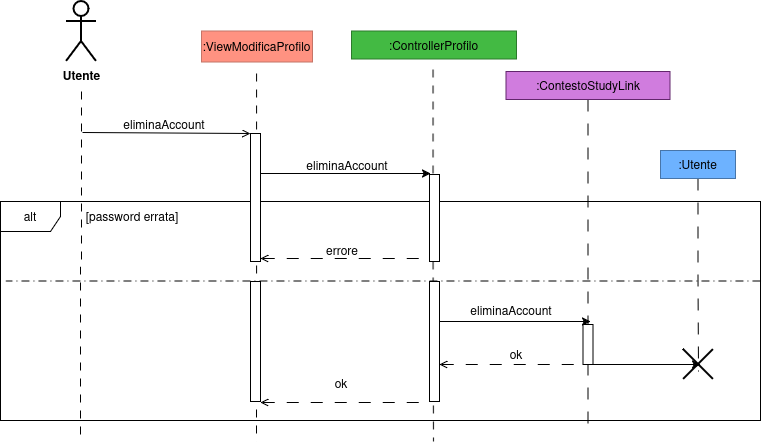
\includegraphics[width=\textwidth,height=0.5\textheight,keepaspectratio]{images/interazione-progettazione-elimina-account.png}
    \caption{Diagramma di sequenza: Elimina account}
\end{figure}
%
\subsubsection{Interazione: Gestione evento}
Di seguito sono presentate le figure che mostrano le interazioni tra i componenti per la gestione degli eventi. Per brevità e per mostrare le differenze con quelli mostrati in analisi, si è riportato solo il caso della creazione e della gestione dell'evento.
Anche se non è indicato nel diagramma, per motivi di spazio, ci sarà la memorizzazione dei dati sul database.

\begin{figure}[H]
    \centering
    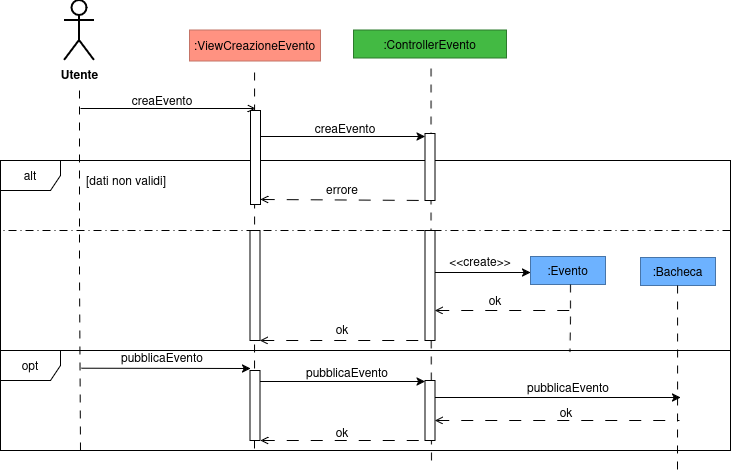
\includegraphics[width=\textwidth,height=0.5\textheight,keepaspectratio]{images/interazione-progettazione-creazione-evento.png}
    \caption{Diagramma di sequenza: Gestione evento - Creazione}
\end{figure}
%
\begin{figure}[H]
    \centering
    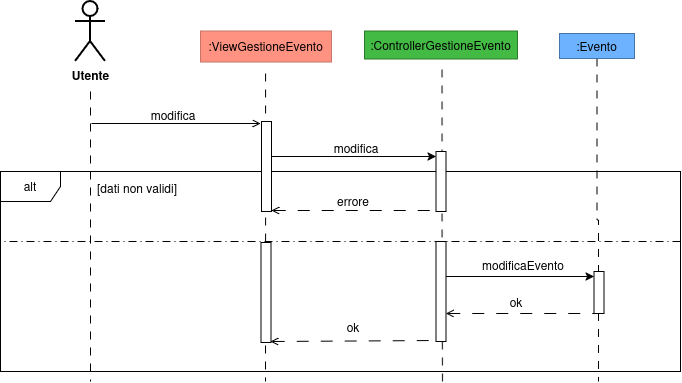
\includegraphics[width=\textwidth,height=0.5\textheight,keepaspectratio]{images/interazione-progettazione-gestione-evento.png}
    \caption{Diagramma di sequenza: Gestione evento - Gestione}
\end{figure}
%
\subsubsection{Interazione: Elimina evento}
Si omette il diagramma relativo all'eliminazione dell'evento in quanto il suo flusso di interazione risulta essere praticamente identico a quello della modifica dell'evento, differendo unicamente nell'operazione finale di eliminazione dell'entità anziché di aggiornamento.
%
\subsubsection{Interazione: Bacheca}
Di seguito è presentata la figura che mostra le interazioni tra i componenti per il filtraggio degli eventi in bacheca.

\begin{figure}[H]
    \centering
    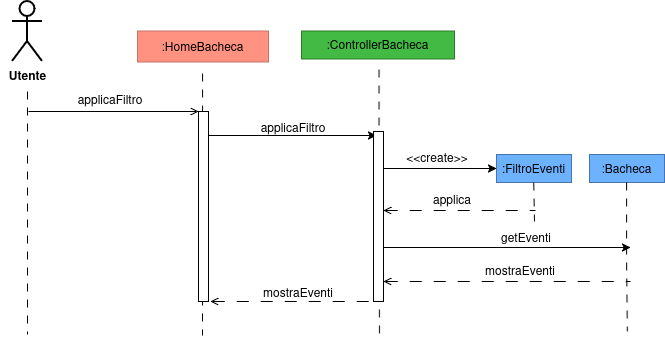
\includegraphics[width=\textwidth,height=0.5\textheight,keepaspectratio]{images/interazione-progettazione-filtro-eventi.png}
    \caption{Diagramma di sequenza: Bacheca - Filtro eventi}
\end{figure}
%
\subsubsection{Interazione: Comunicazione}
Di seguito sono presentate le figure che mostrano le interazioni tra i componenti per la comunicazione tra gli utenti tramite chat e commenti.

\begin{figure}[H]
    \centering
    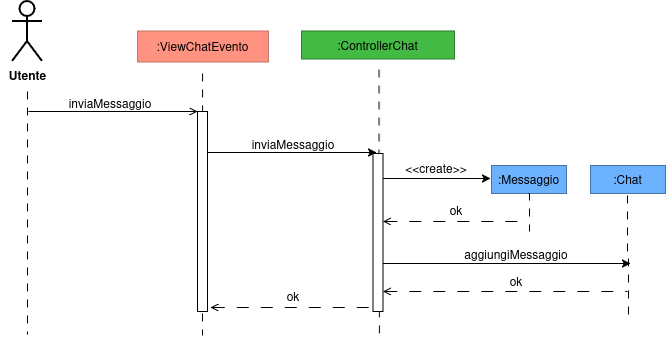
\includegraphics[width=\textwidth,height=0.5\textheight,keepaspectratio]{images/interazione-progettazione-chat.png}
    \caption{Diagramma di sequenza: Comunicazione - Chat}
\end{figure}
%
\begin{figure}[H]
    \centering
    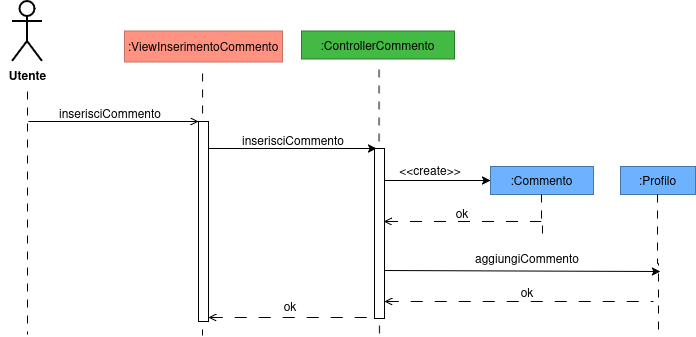
\includegraphics[width=\textwidth,height=0.5\textheight,keepaspectratio]{images/interazione-progettazione-commento.png}
    \caption{Diagramma di sequenza: Comunicazione - Commento}
\end{figure}
%


\newpage
\subsection{Interfacce utente}
Nelle prossime sezioni mostreremo le interfacce principali del sistema.
Visto lo scopo dell'applicazione, prevediamo che gli utenti la useranno quasi sempre dal telefono.
Per questo motivo, in questo documento abbiamo deciso di inserire solo le schermate della versione per smartphone.

Non abbiamo messo la versione per computer perché è molto facile da immaginare: si tratta semplicemente della stessa grafica 
allargata e riadattata per uno schermo più grande.

\begin{figure}[H]
    \centering
    \setlength{\fboxsep}{0pt}
    \setlength{\fboxrule}{1.5pt}
    \begin{minipage}{0.45\textwidth}
        \centering
        \fcolorbox{linkColor}{white}{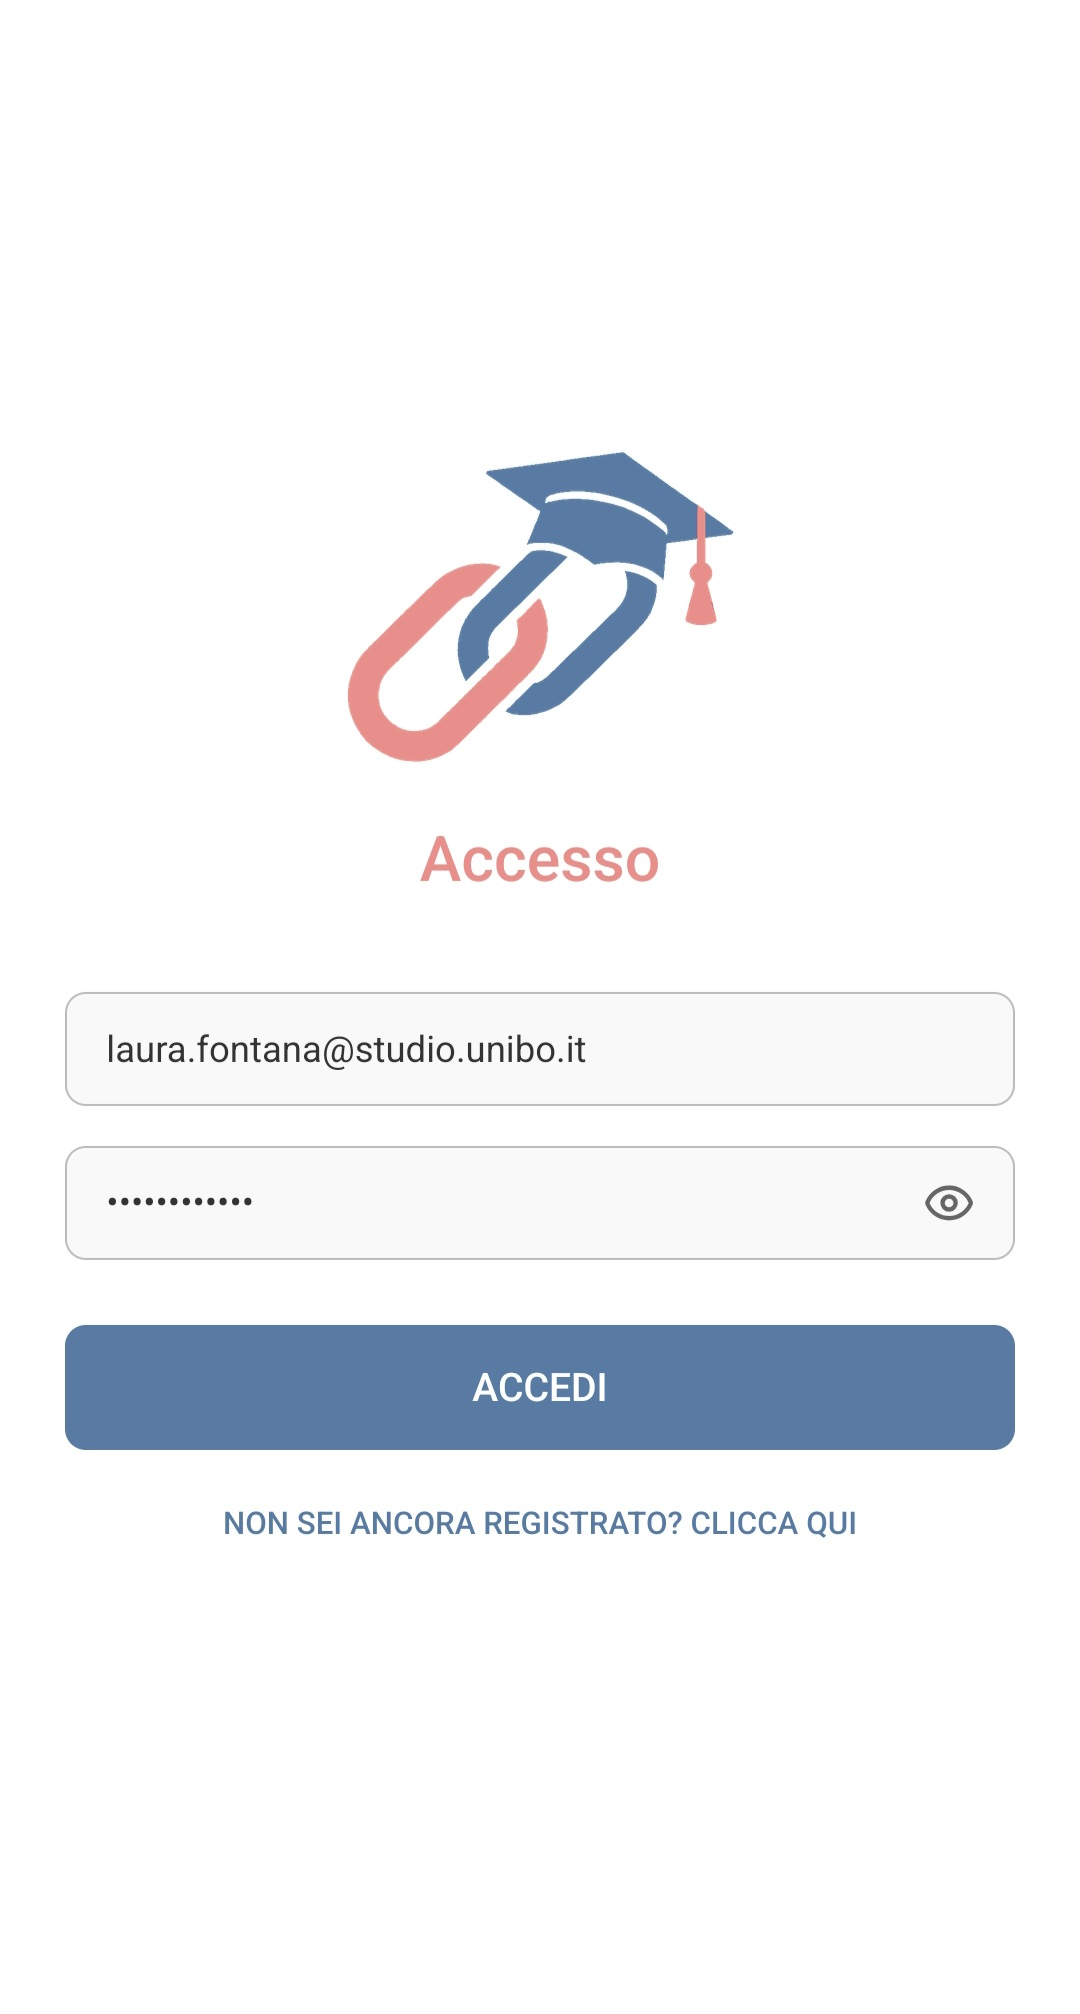
\includegraphics[width=0.98\linewidth,height=0.30\textheight,keepaspectratio]{images/login.jpg}}
        \caption{Schermata di Accesso}
    \end{minipage}\hfill
    \begin{minipage}{0.45\textwidth}
        \centering
        \fcolorbox{linkColor}{white}{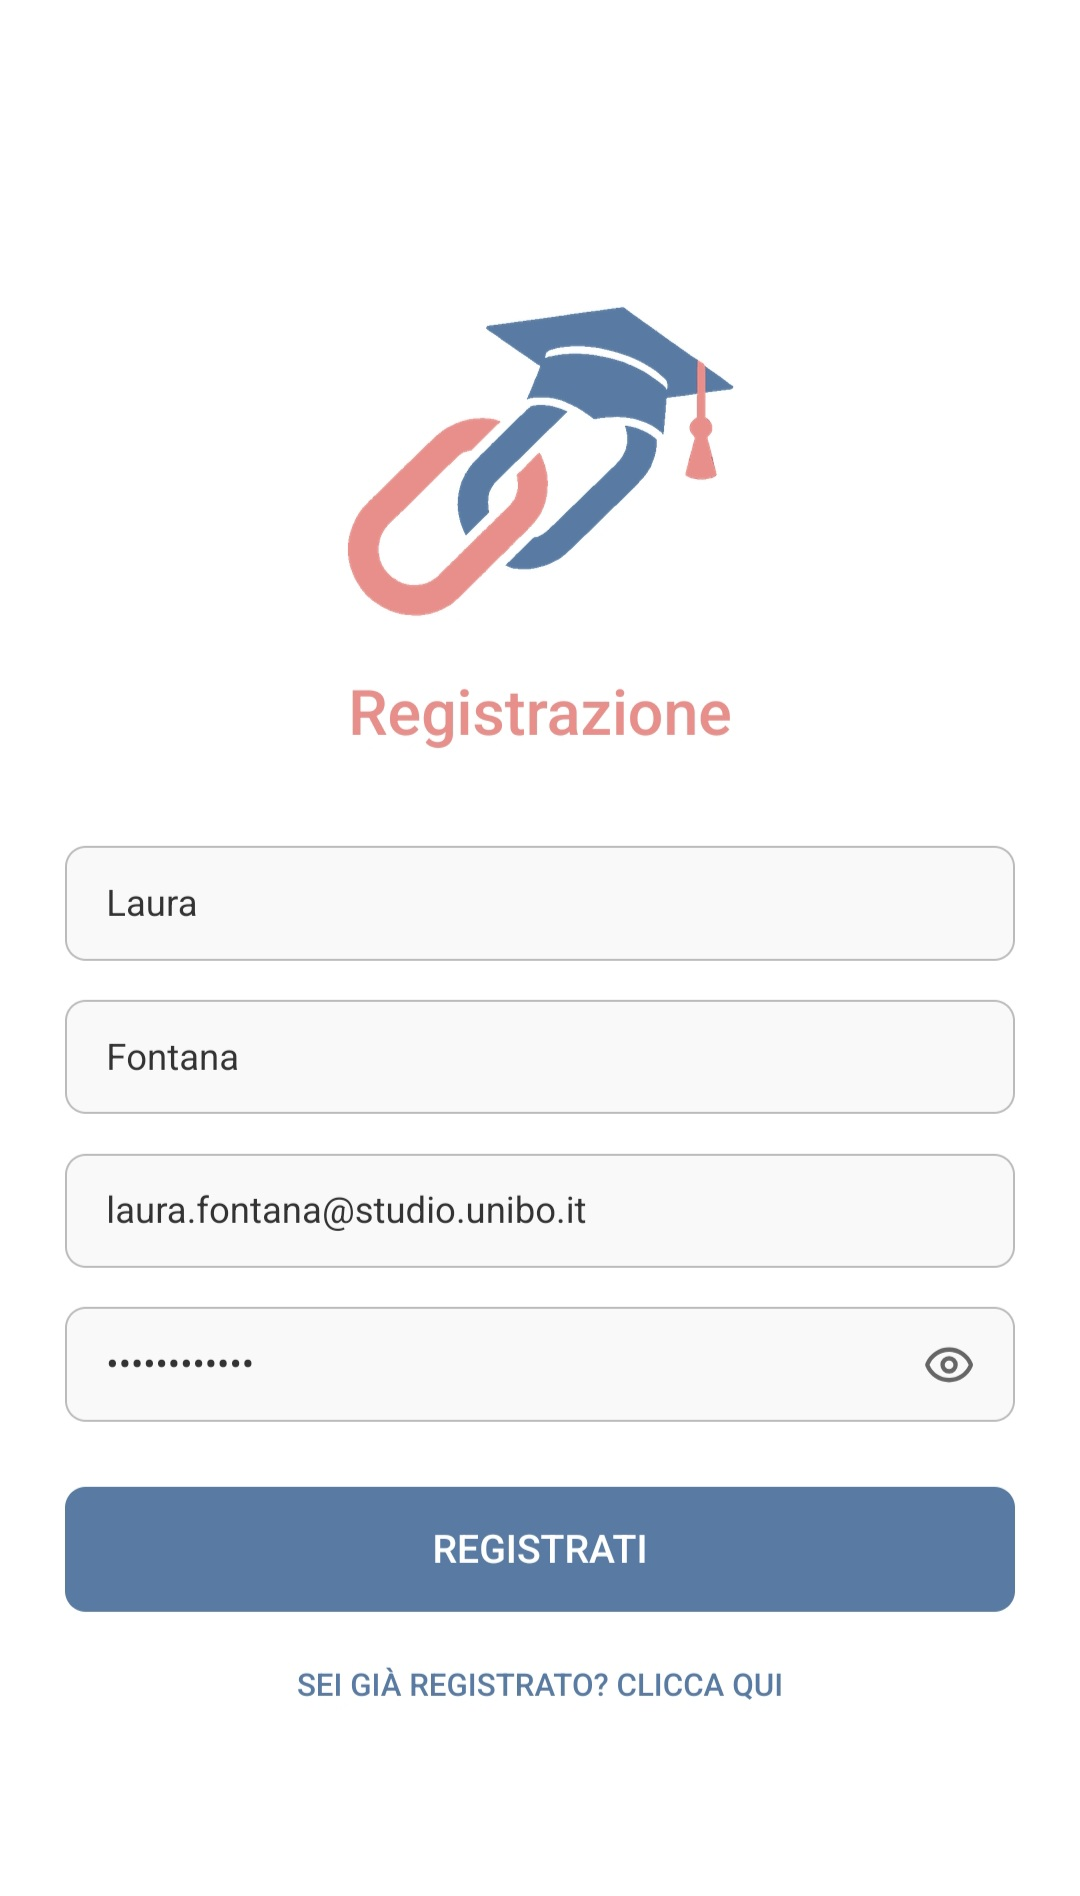
\includegraphics[width=0.98\linewidth,height=0.30\textheight,keepaspectratio]{images/registrazione.jpg}}
        \caption{Schermata di Registrazione}
    \end{minipage}
\end{figure}

\begin{figure}[H]
    \centering
    \setlength{\fboxsep}{0pt}
    \setlength{\fboxrule}{1.5pt}
    \begin{minipage}{0.31\textwidth}
        \centering
        \fcolorbox{linkColor}{white}{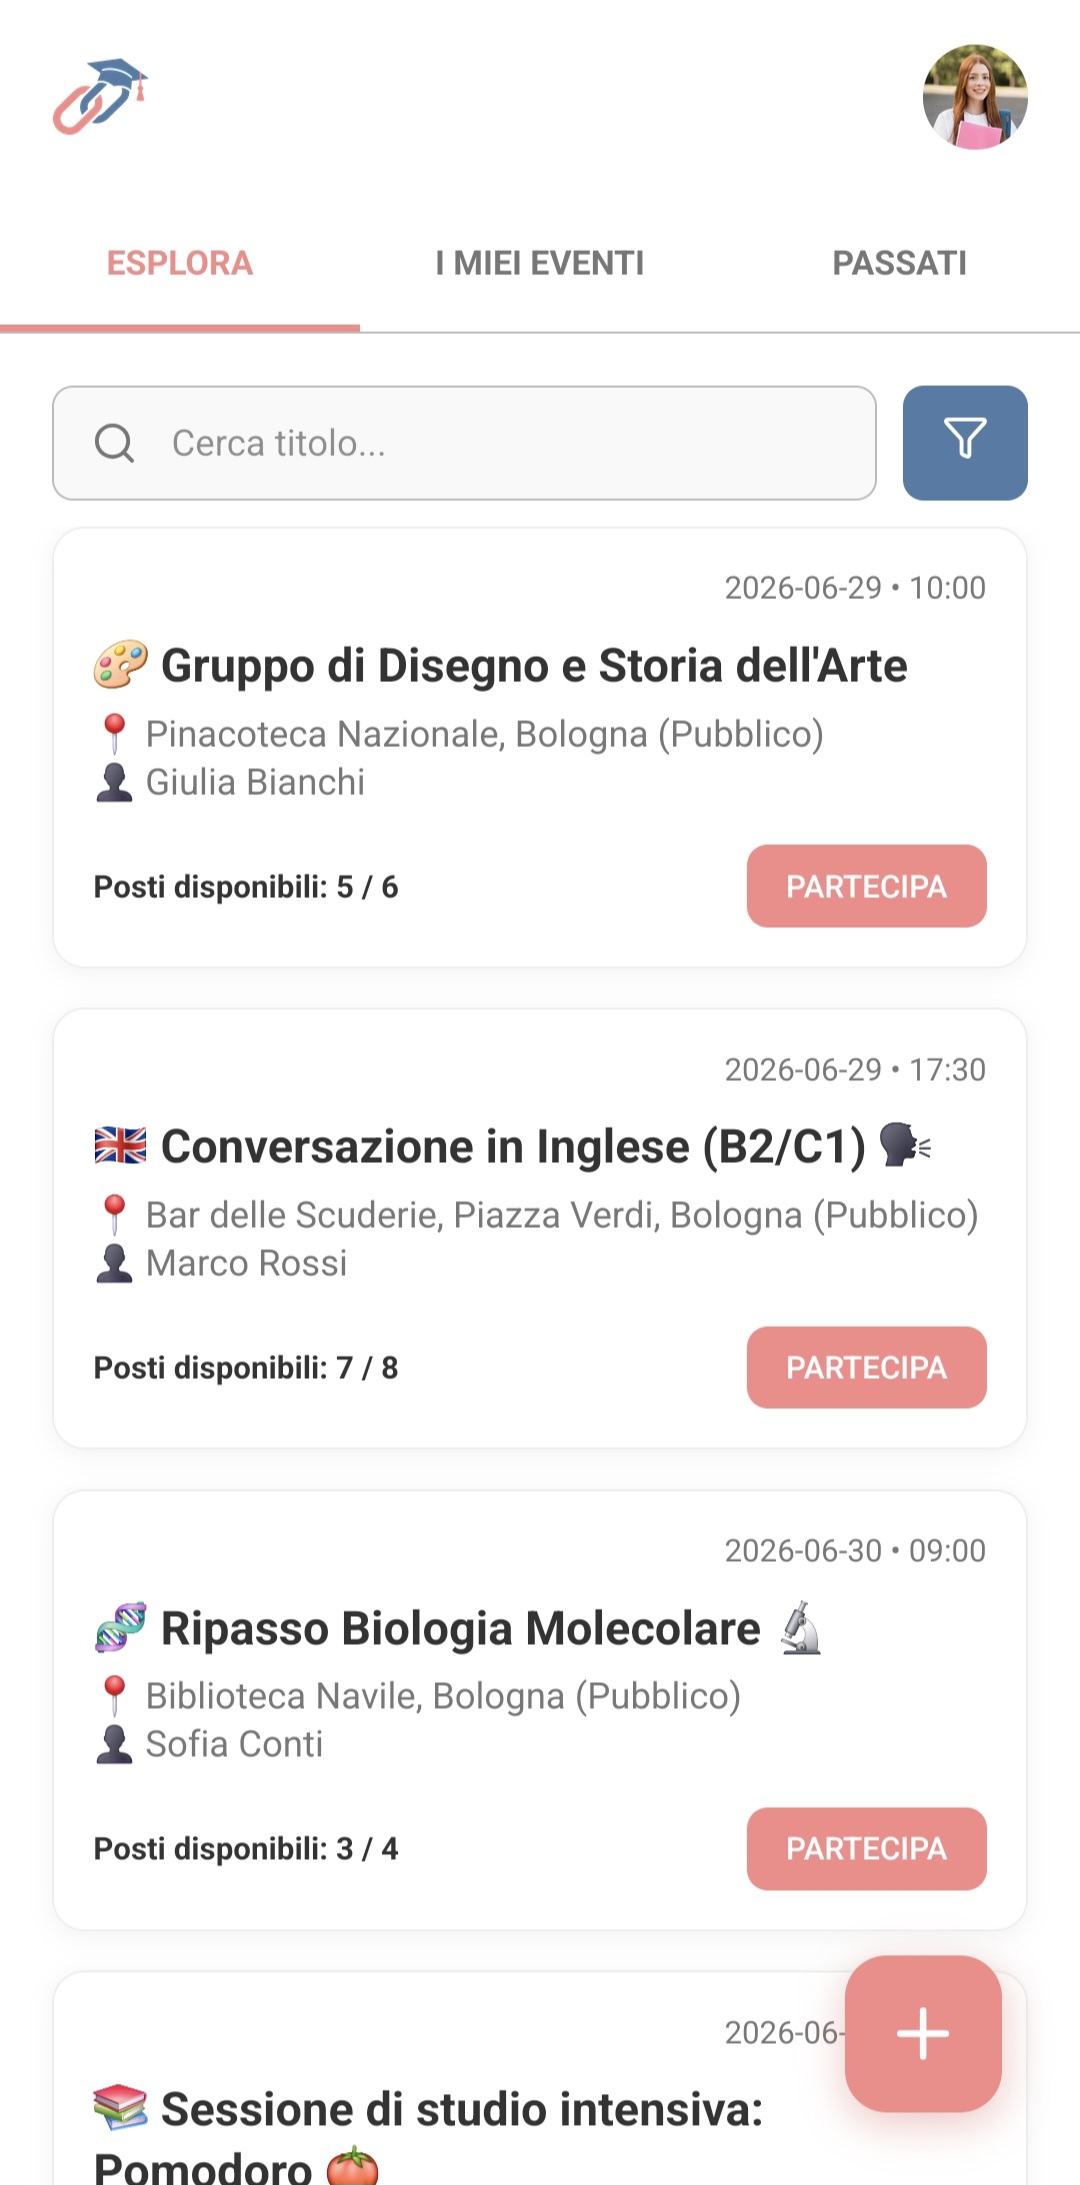
\includegraphics[width=0.98\linewidth,height=0.30\textheight,keepaspectratio]{images/bacheca.jpg}}
        \caption{Bacheca - Esplora}
    \end{minipage}\hfill
    \begin{minipage}{0.31\textwidth}
        \centering
        \fcolorbox{linkColor}{white}{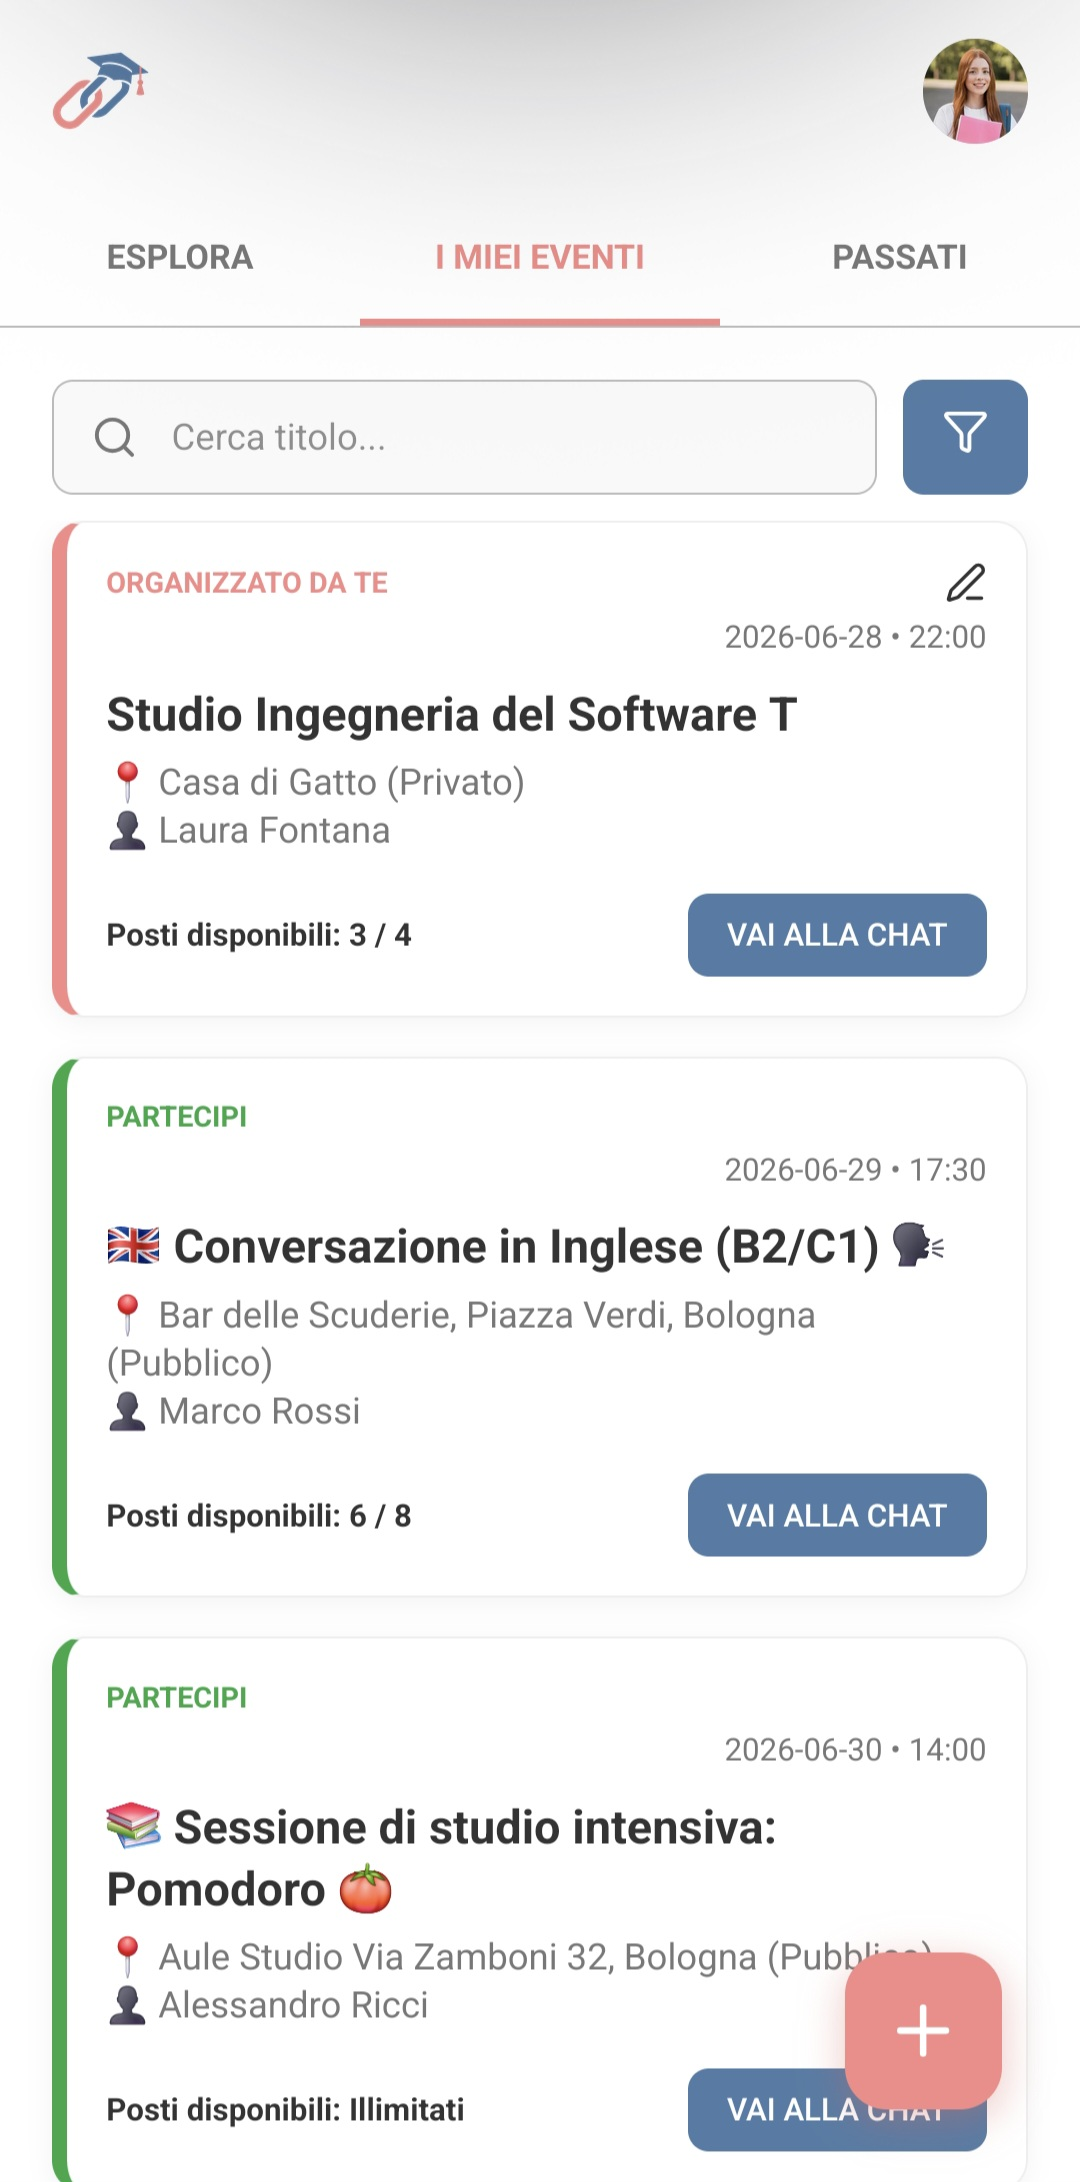
\includegraphics[width=0.98\linewidth,height=0.30\textheight,keepaspectratio]{images/miei-eventi.jpg}}
        \caption{Bacheca - I Miei Eventi}
    \end{minipage}\hfill
    \begin{minipage}{0.31\textwidth}
        \centering
        \fcolorbox{linkColor}{white}{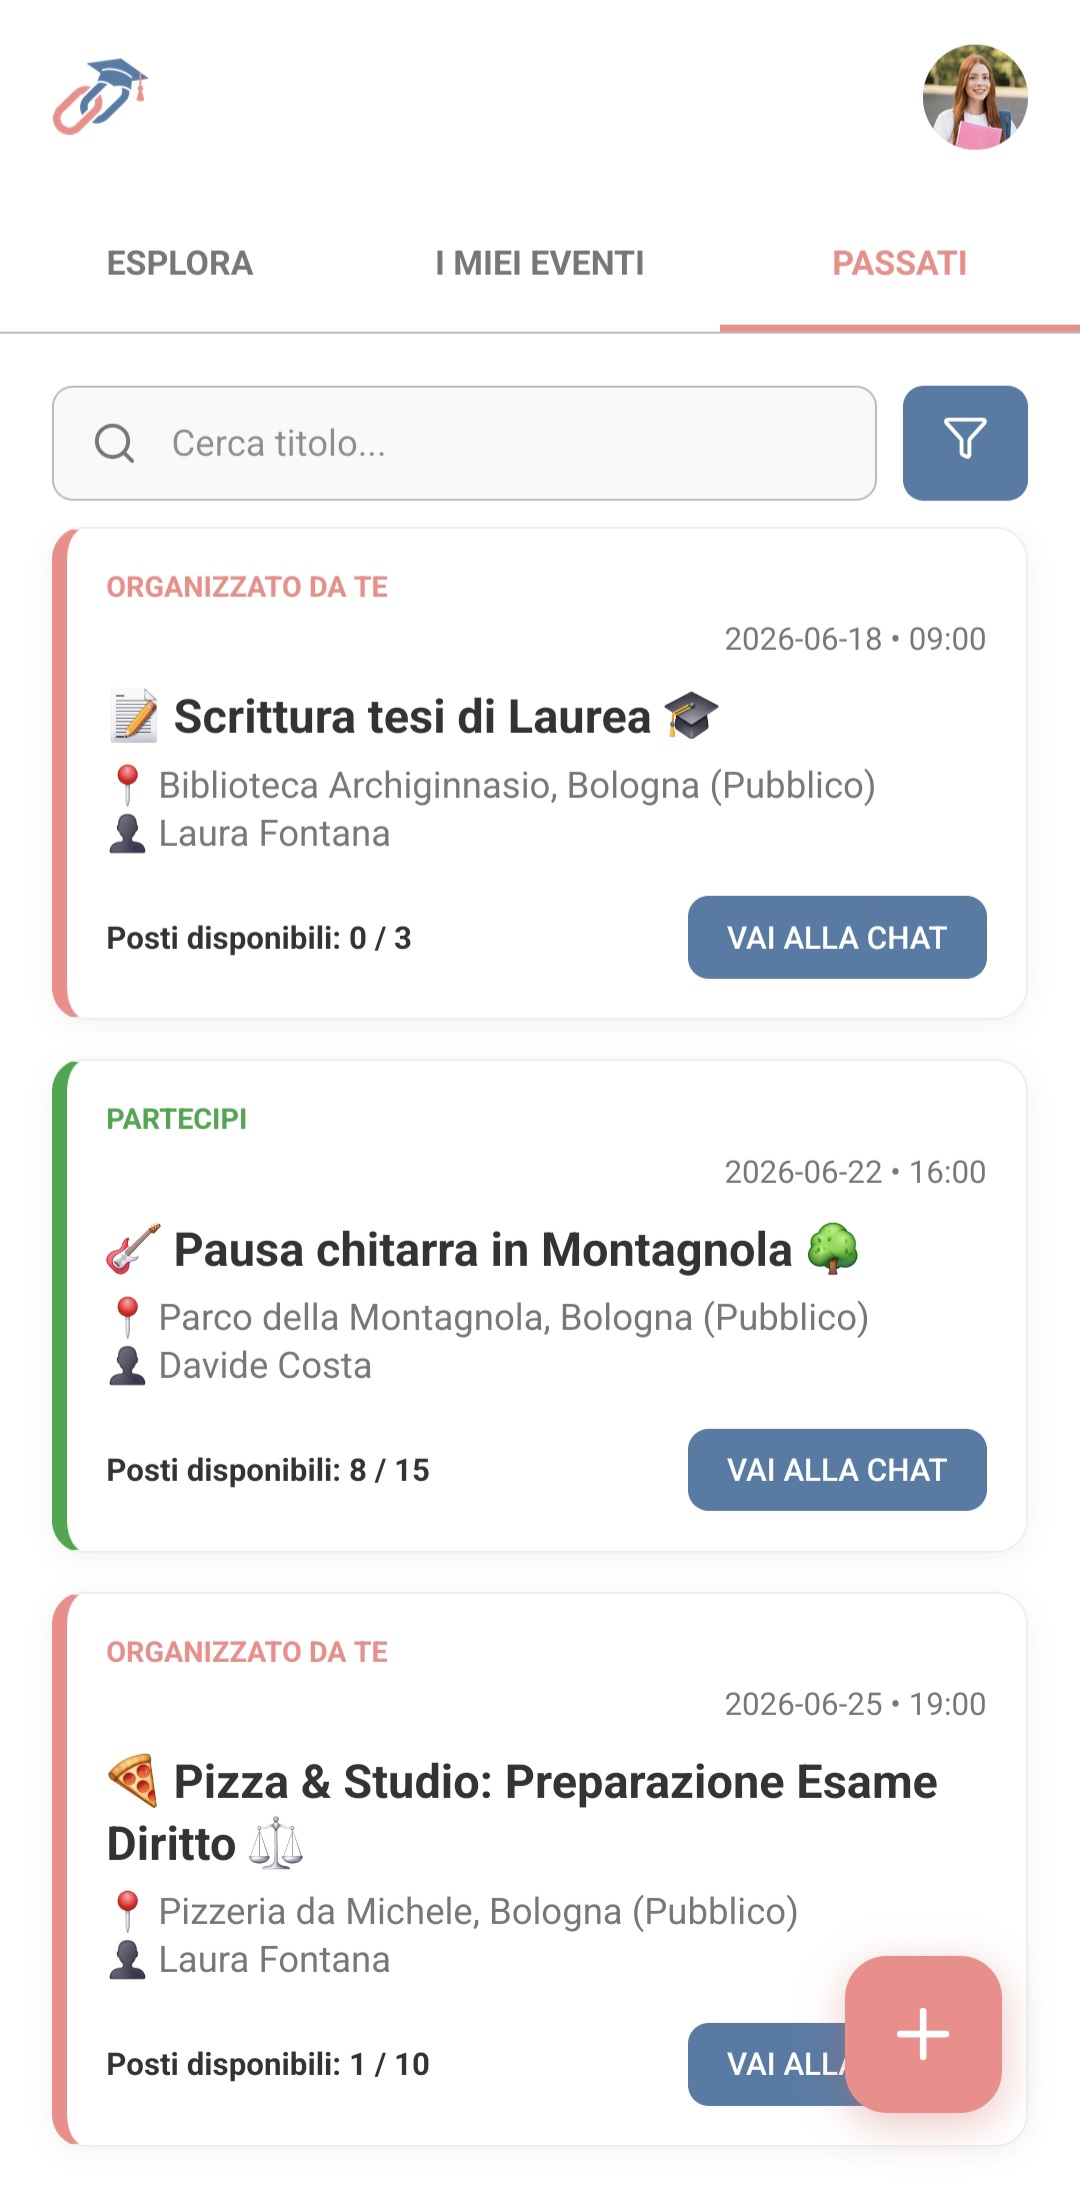
\includegraphics[width=0.98\linewidth,height=0.30\textheight,keepaspectratio]{images/passati.jpg}}
        \caption{Bacheca - Eventi Passati}
    \end{minipage}
\end{figure}

\begin{figure}[H]
    \centering
    \setlength{\fboxsep}{0pt}
    \setlength{\fboxrule}{1.5pt}
    \begin{minipage}{0.45\textwidth}
        \centering
        \fcolorbox{linkColor}{white}{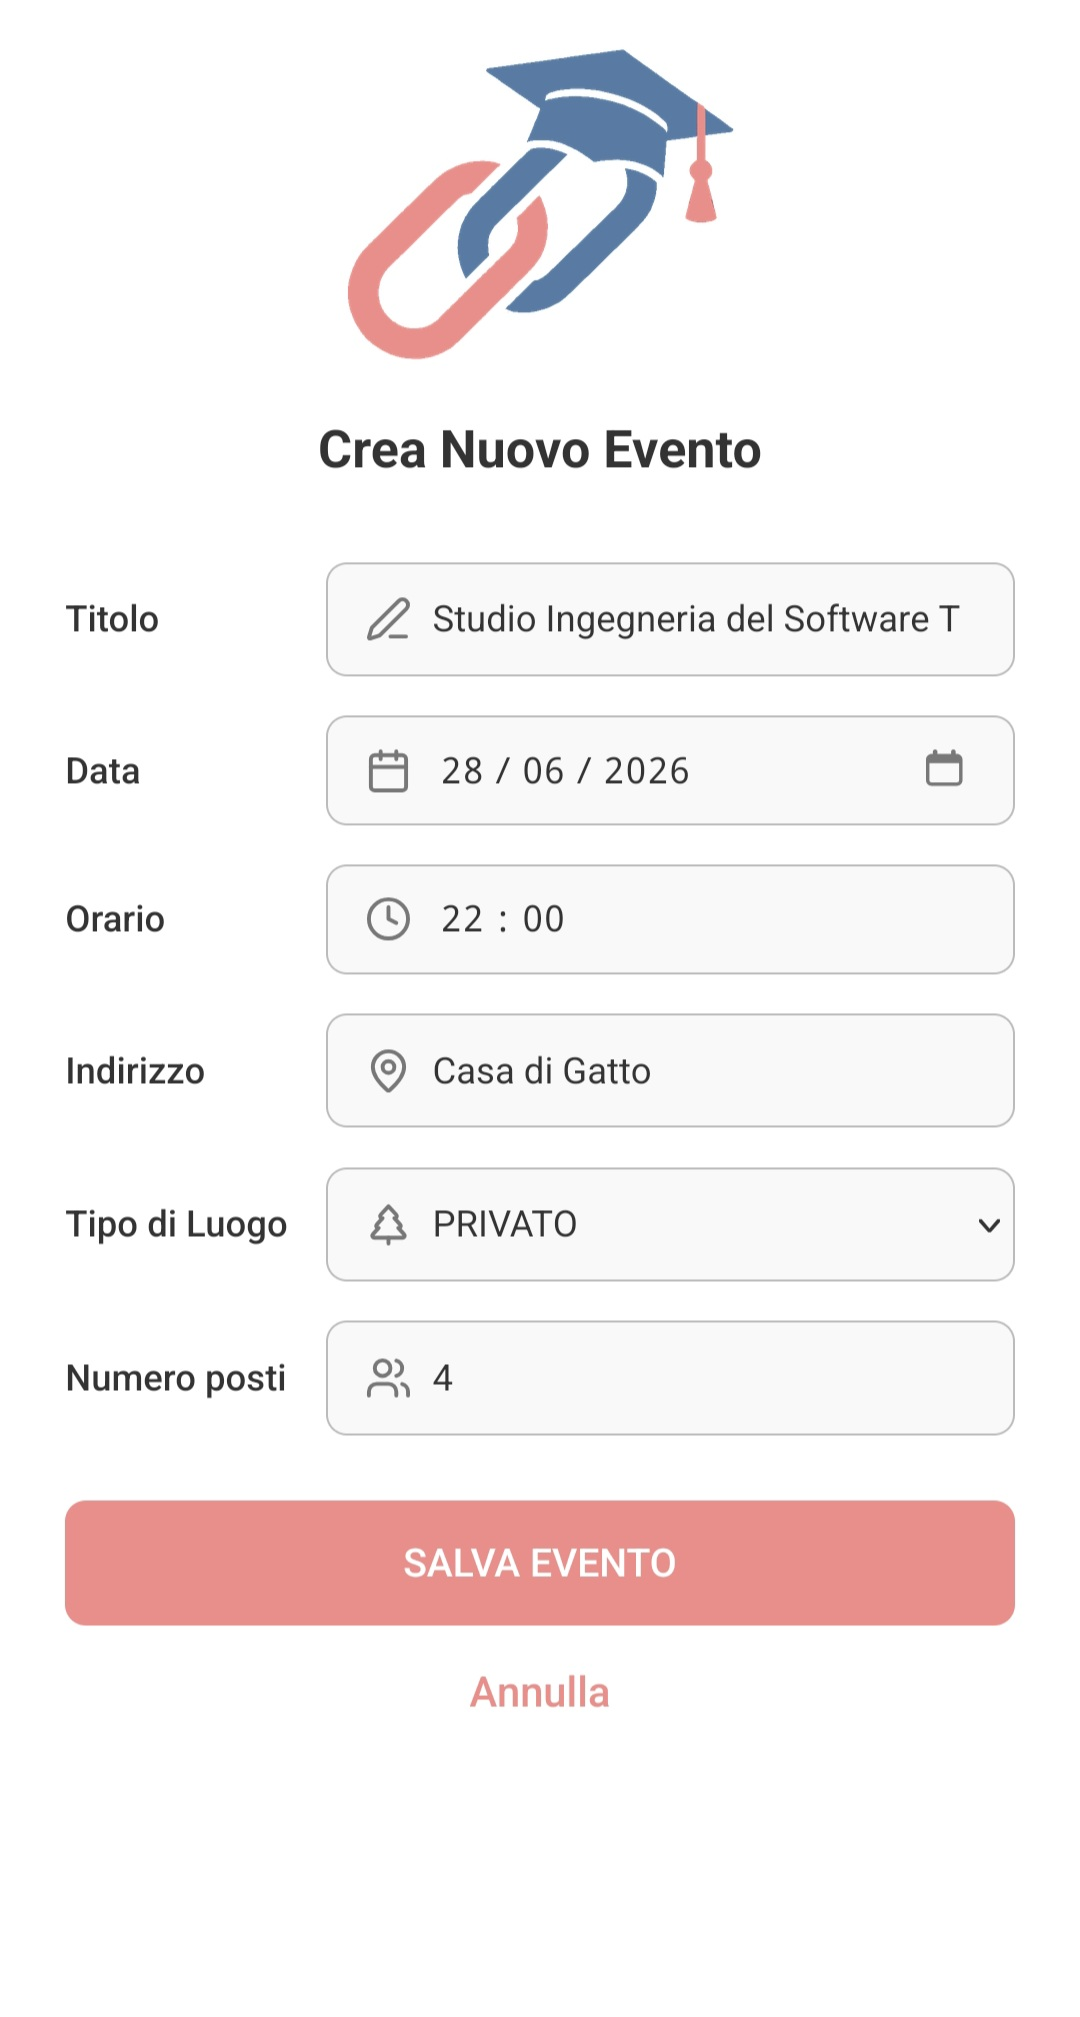
\includegraphics[width=0.98\linewidth,height=0.30\textheight,keepaspectratio]{images/crea-evento.jpg}}
        \caption{Creazione Evento}
    \end{minipage}\hfill
    \begin{minipage}{0.45\textwidth}
        \centering
        \fcolorbox{linkColor}{white}{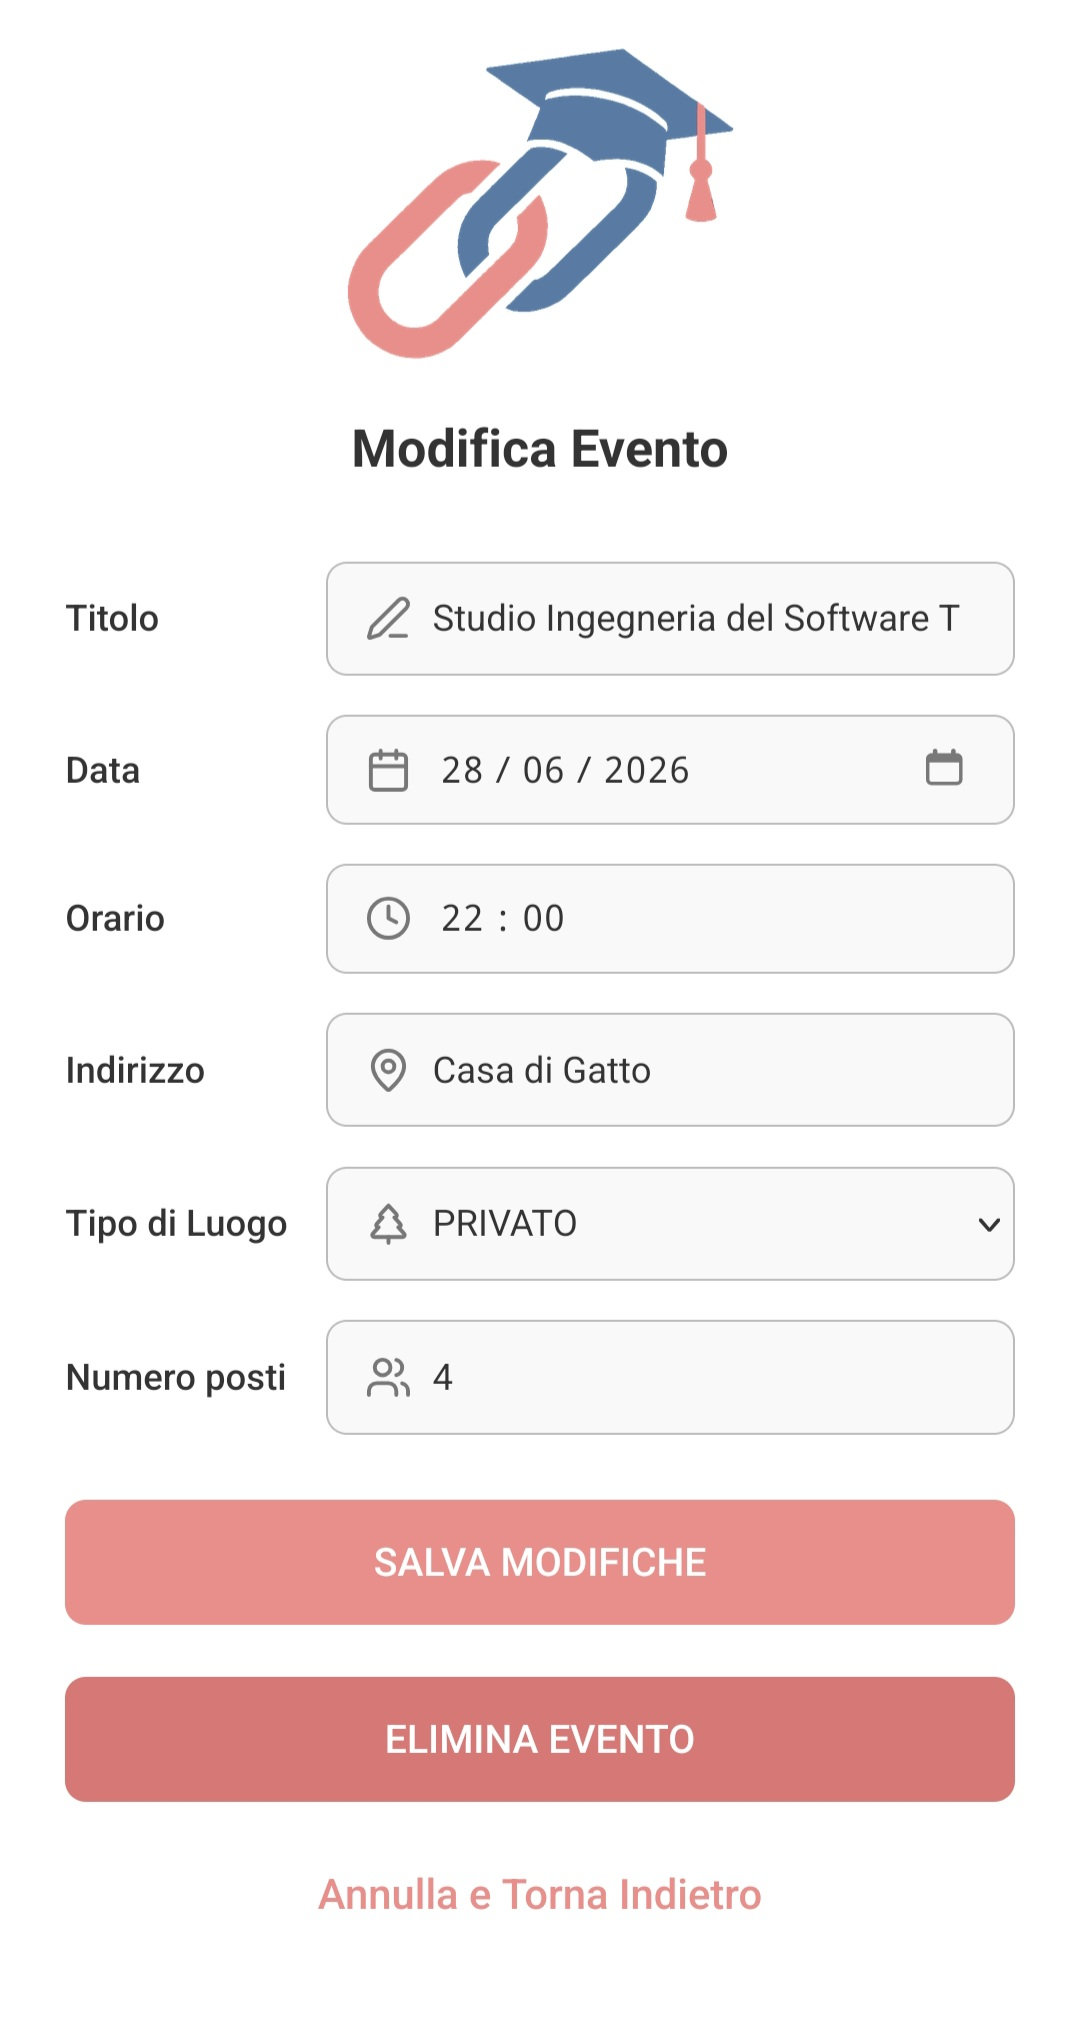
\includegraphics[width=0.98\linewidth,height=0.30\textheight,keepaspectratio]{images/modifica-evento.jpg}}
        \caption{Modifica Evento}
    \end{minipage}
\end{figure}

\begin{figure}[H]
    \centering
    \setlength{\fboxsep}{0pt}
    \setlength{\fboxrule}{1.5pt}
    \begin{minipage}{0.45\textwidth}
        \centering
        \fcolorbox{linkColor}{white}{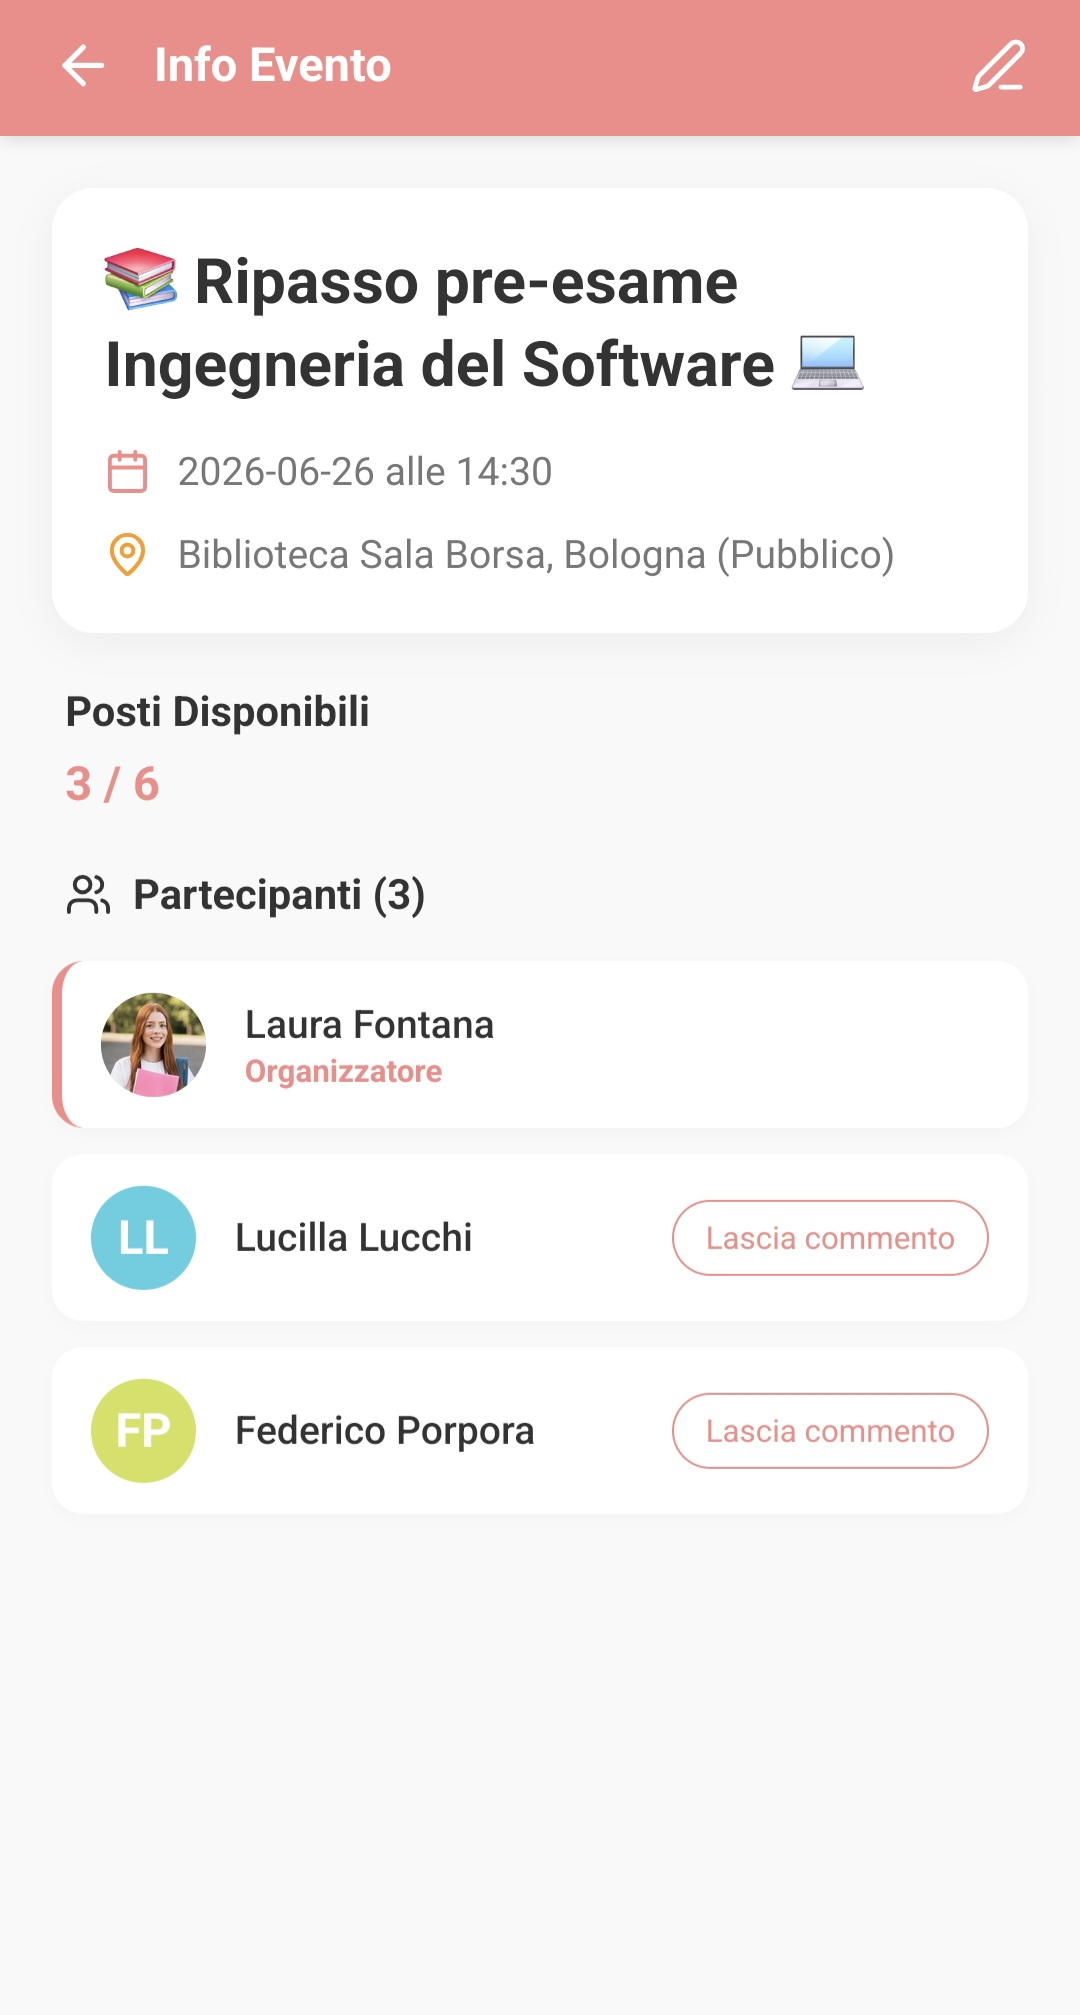
\includegraphics[width=0.98\linewidth,height=0.30\textheight,keepaspectratio]{images/evento-passato.jpg}}
        \caption{Dettagli Evento Passato}
    \end{minipage}\hfill
    \begin{minipage}{0.45\textwidth}
        \centering
        \fcolorbox{linkColor}{white}{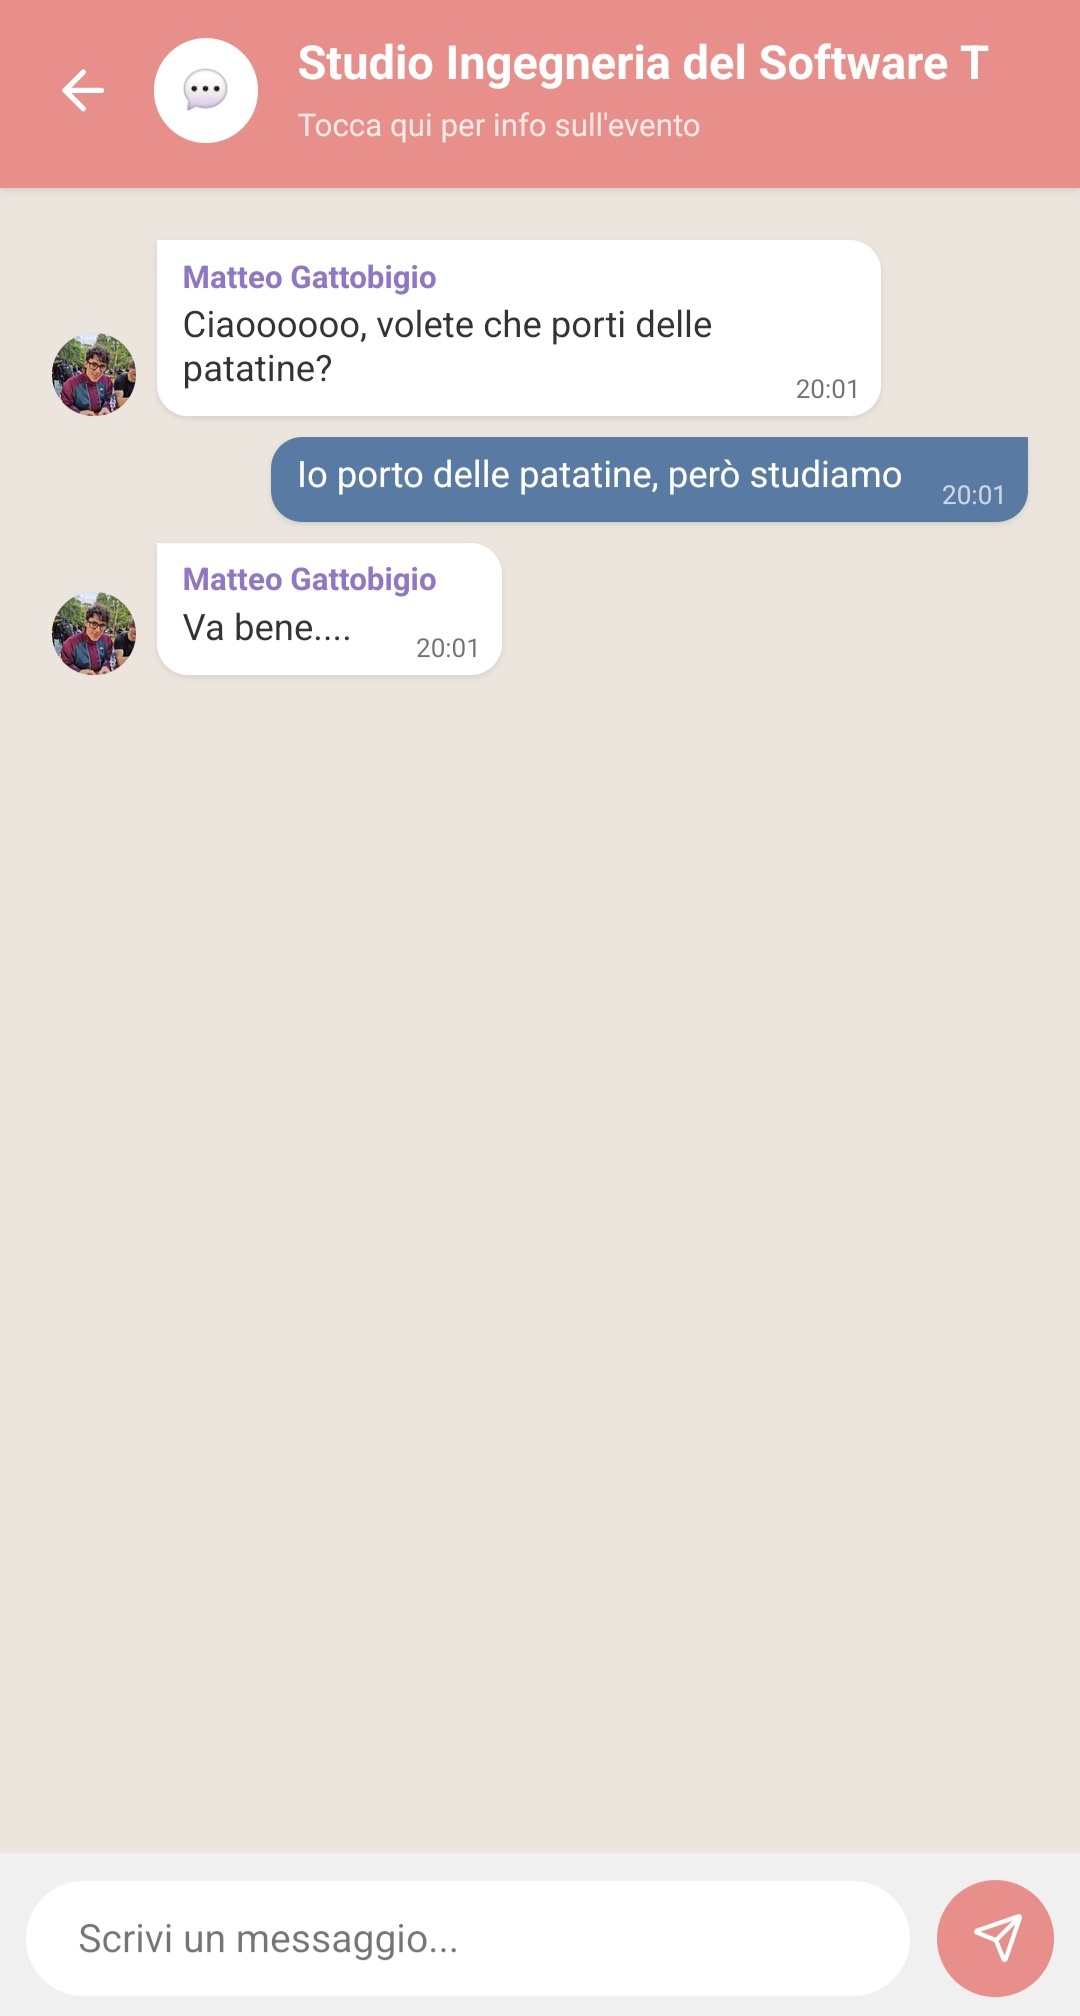
\includegraphics[width=0.98\linewidth,height=0.30\textheight,keepaspectratio]{images/chat.jpg}}
        \caption{Chat di Gruppo}
    \end{minipage}
\end{figure}

\begin{figure}[H]
    \centering
    \setlength{\fboxsep}{0pt}
    \setlength{\fboxrule}{1.5pt}
    \begin{minipage}{0.45\textwidth}
        \centering
        \fcolorbox{linkColor}{white}{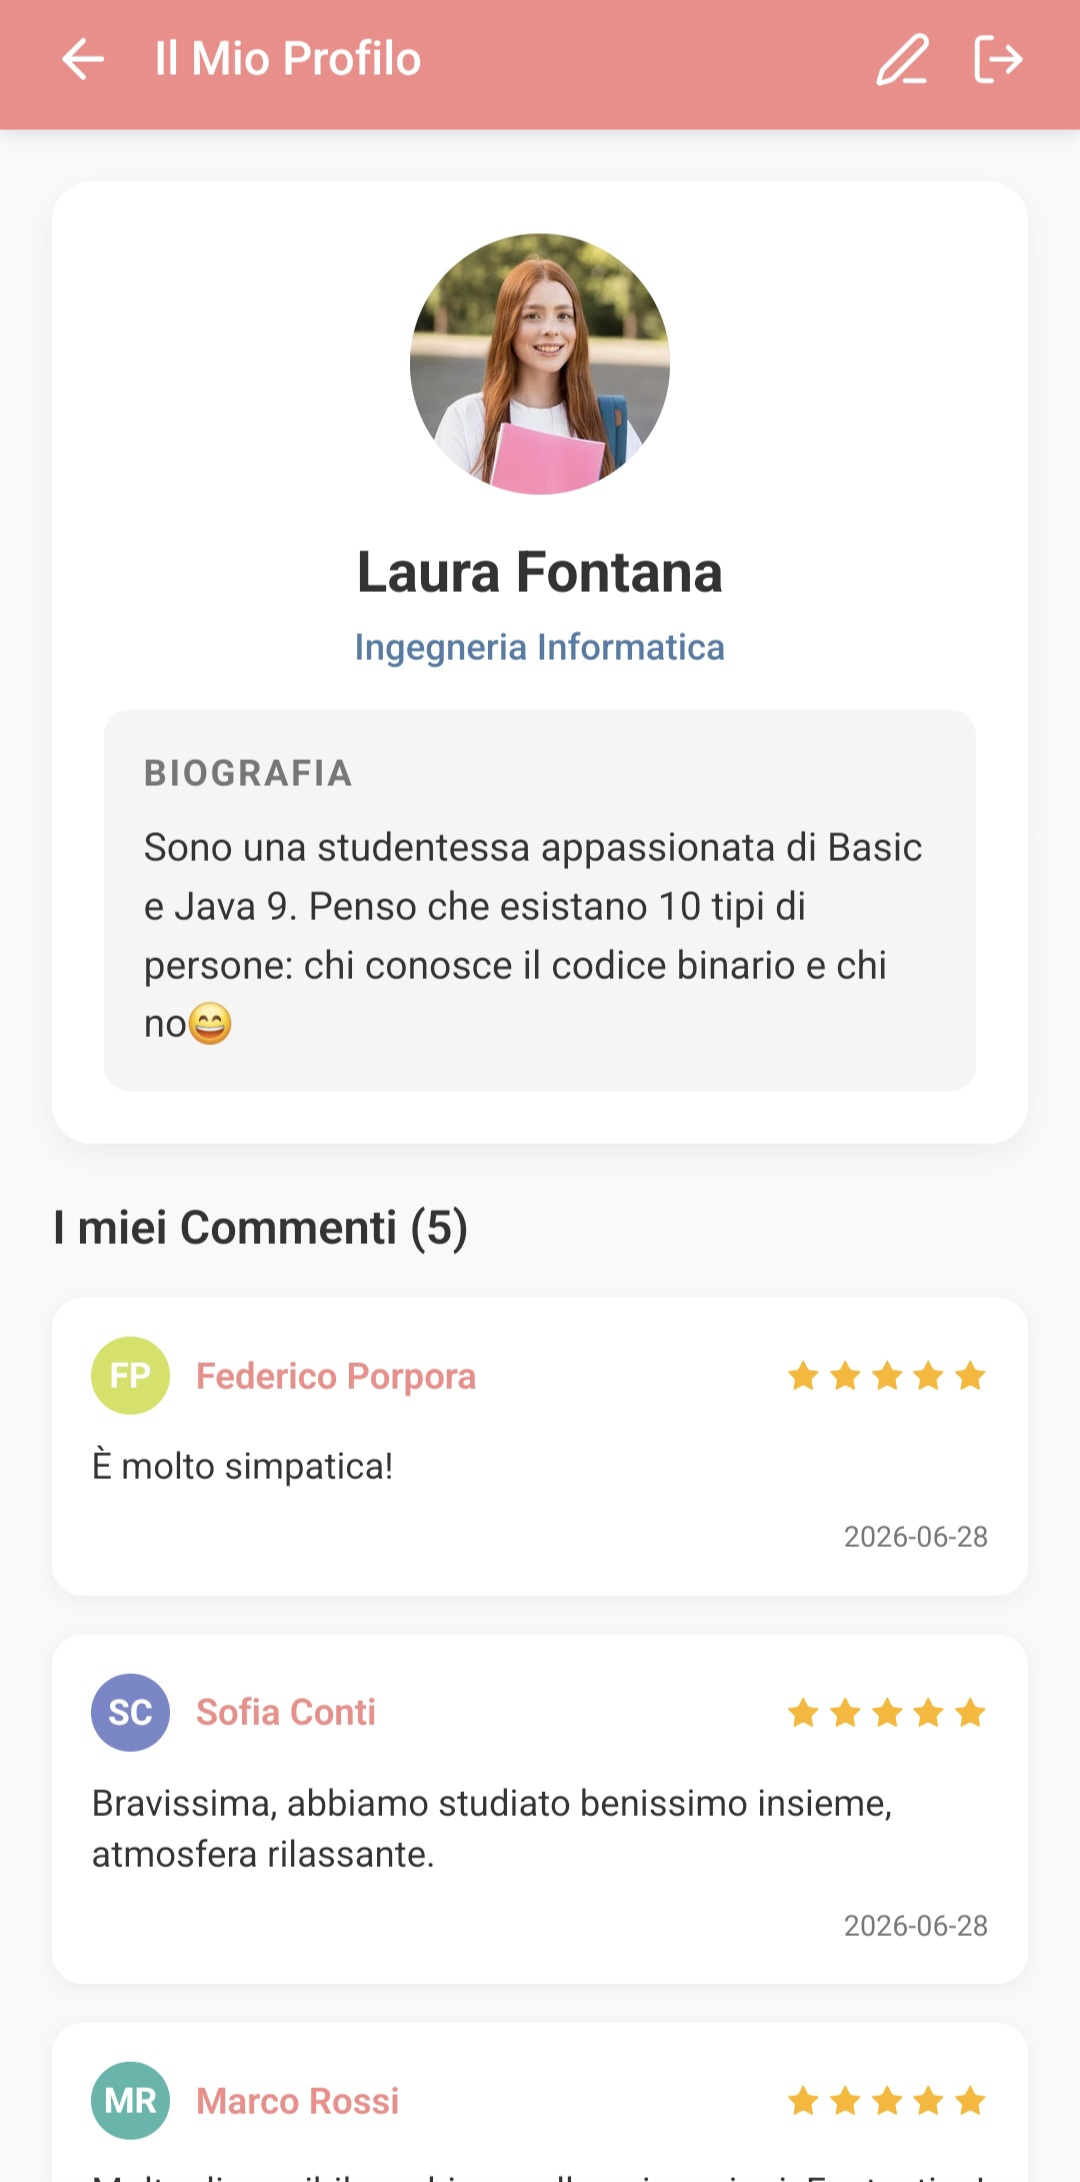
\includegraphics[width=0.98\linewidth,height=0.30\textheight,keepaspectratio]{images/mio-profilo.jpg}}
        \caption{Profilo Personale}
    \end{minipage}\hfill
    \begin{minipage}{0.45\textwidth}
        \centering
        \fcolorbox{linkColor}{white}{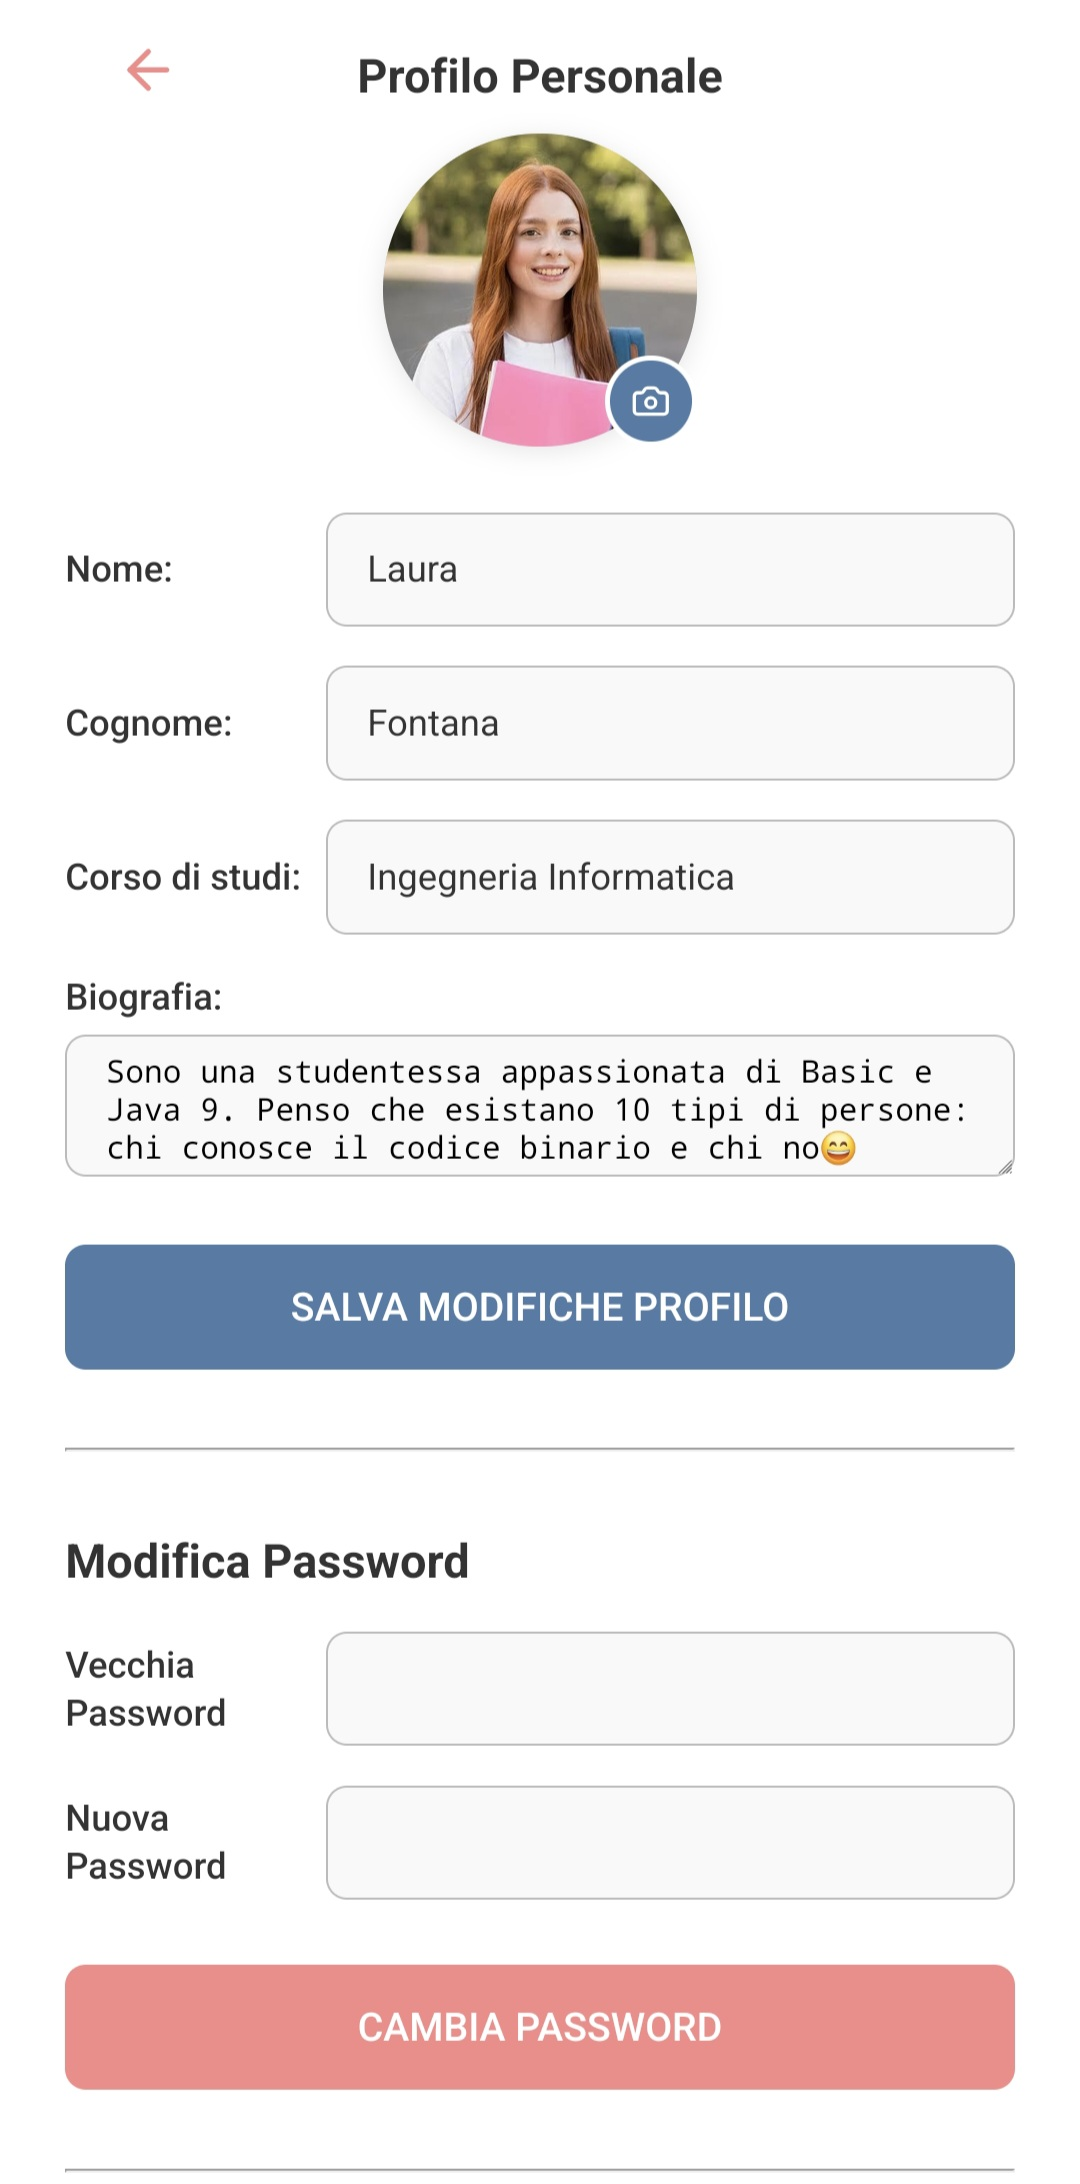
\includegraphics[width=0.98\linewidth,height=0.30\textheight,keepaspectratio]{images/modifica-profilo.jpg}}
        \caption{Modifica Profilo}
    \end{minipage}
\end{figure}

\begin{figure}[H]
    \centering
    \setlength{\fboxsep}{0pt}
    \setlength{\fboxrule}{1.5pt}
    \begin{minipage}{0.45\textwidth}
        \centering
        \fcolorbox{linkColor}{white}{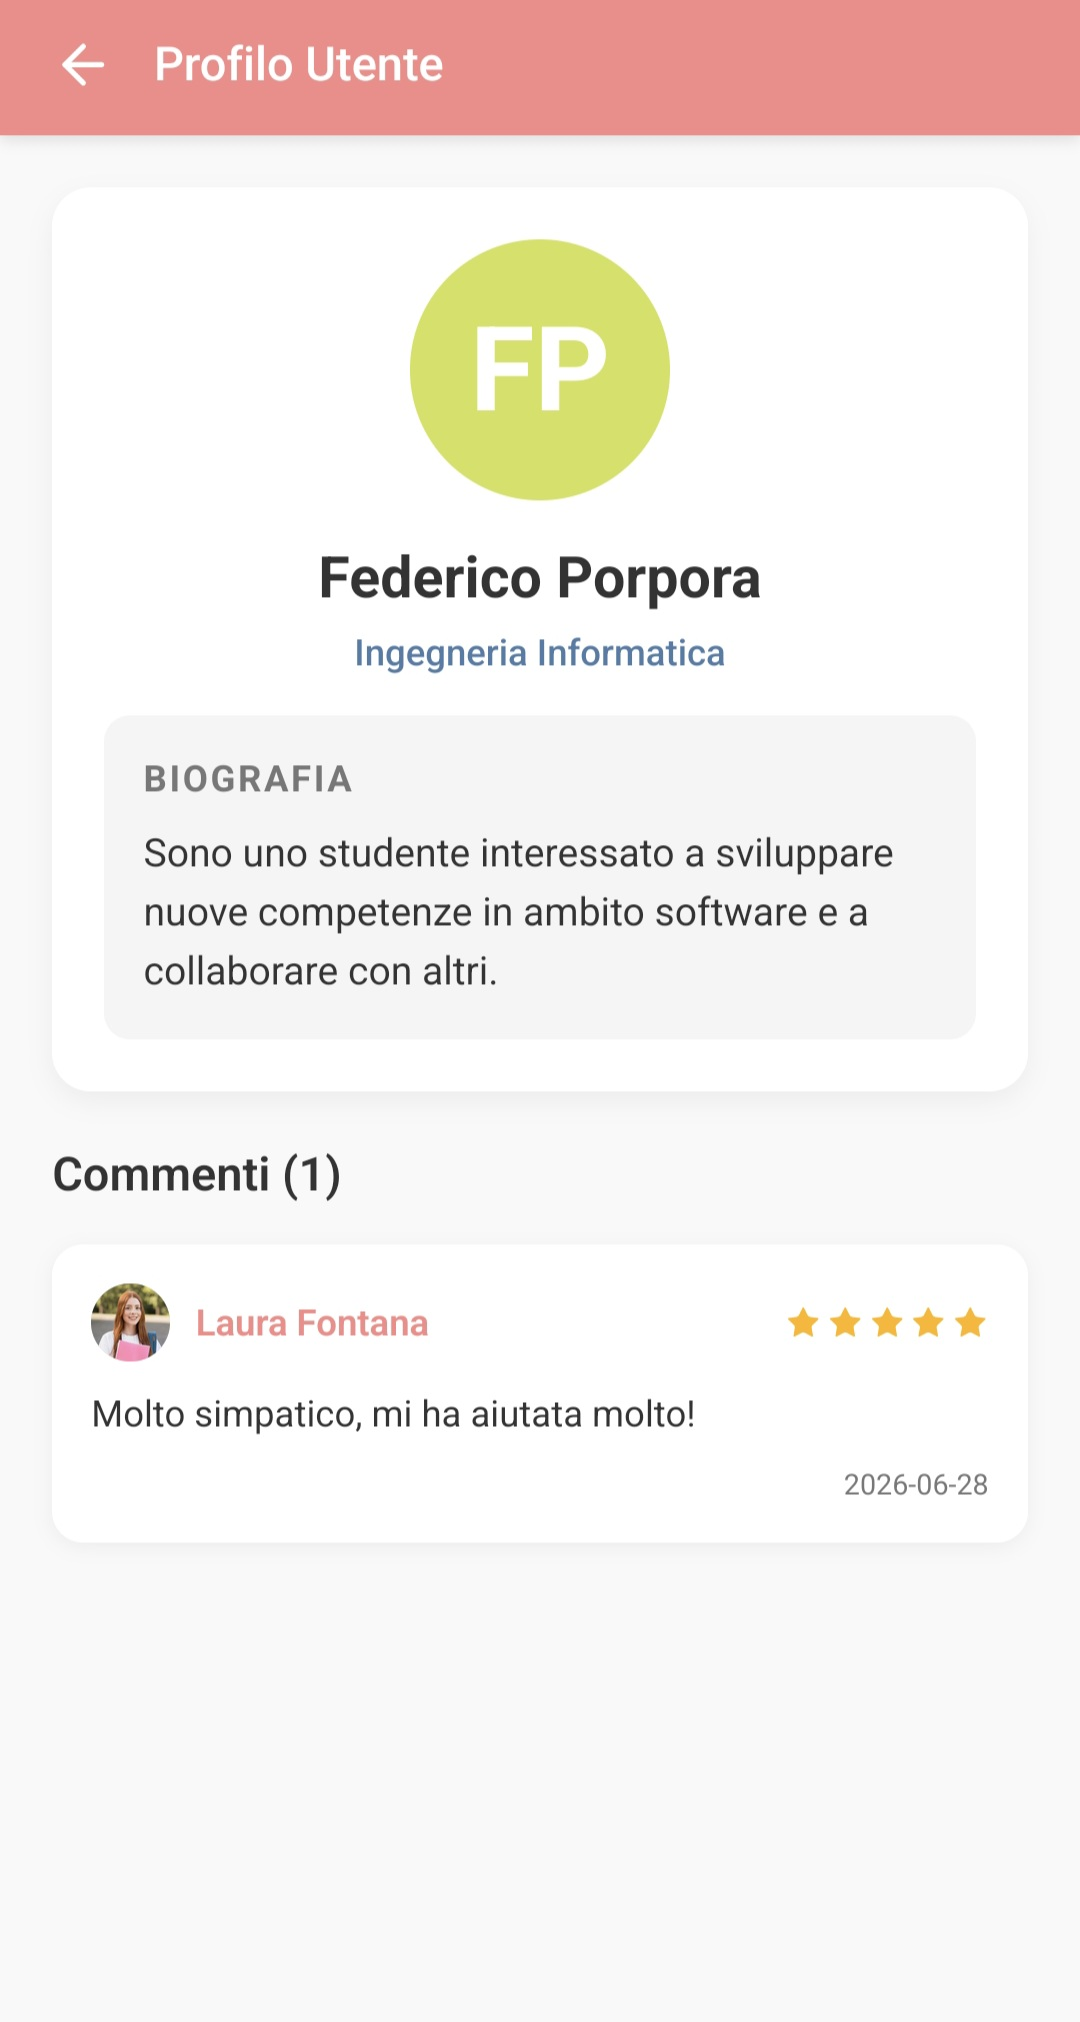
\includegraphics[width=0.98\linewidth,height=0.30\textheight,keepaspectratio]{images/profilo.jpg}}
        \caption{Profilo Pubblico Utente}
    \end{minipage}\hfill
    \begin{minipage}{0.45\textwidth}
        \centering
        \fcolorbox{linkColor}{white}{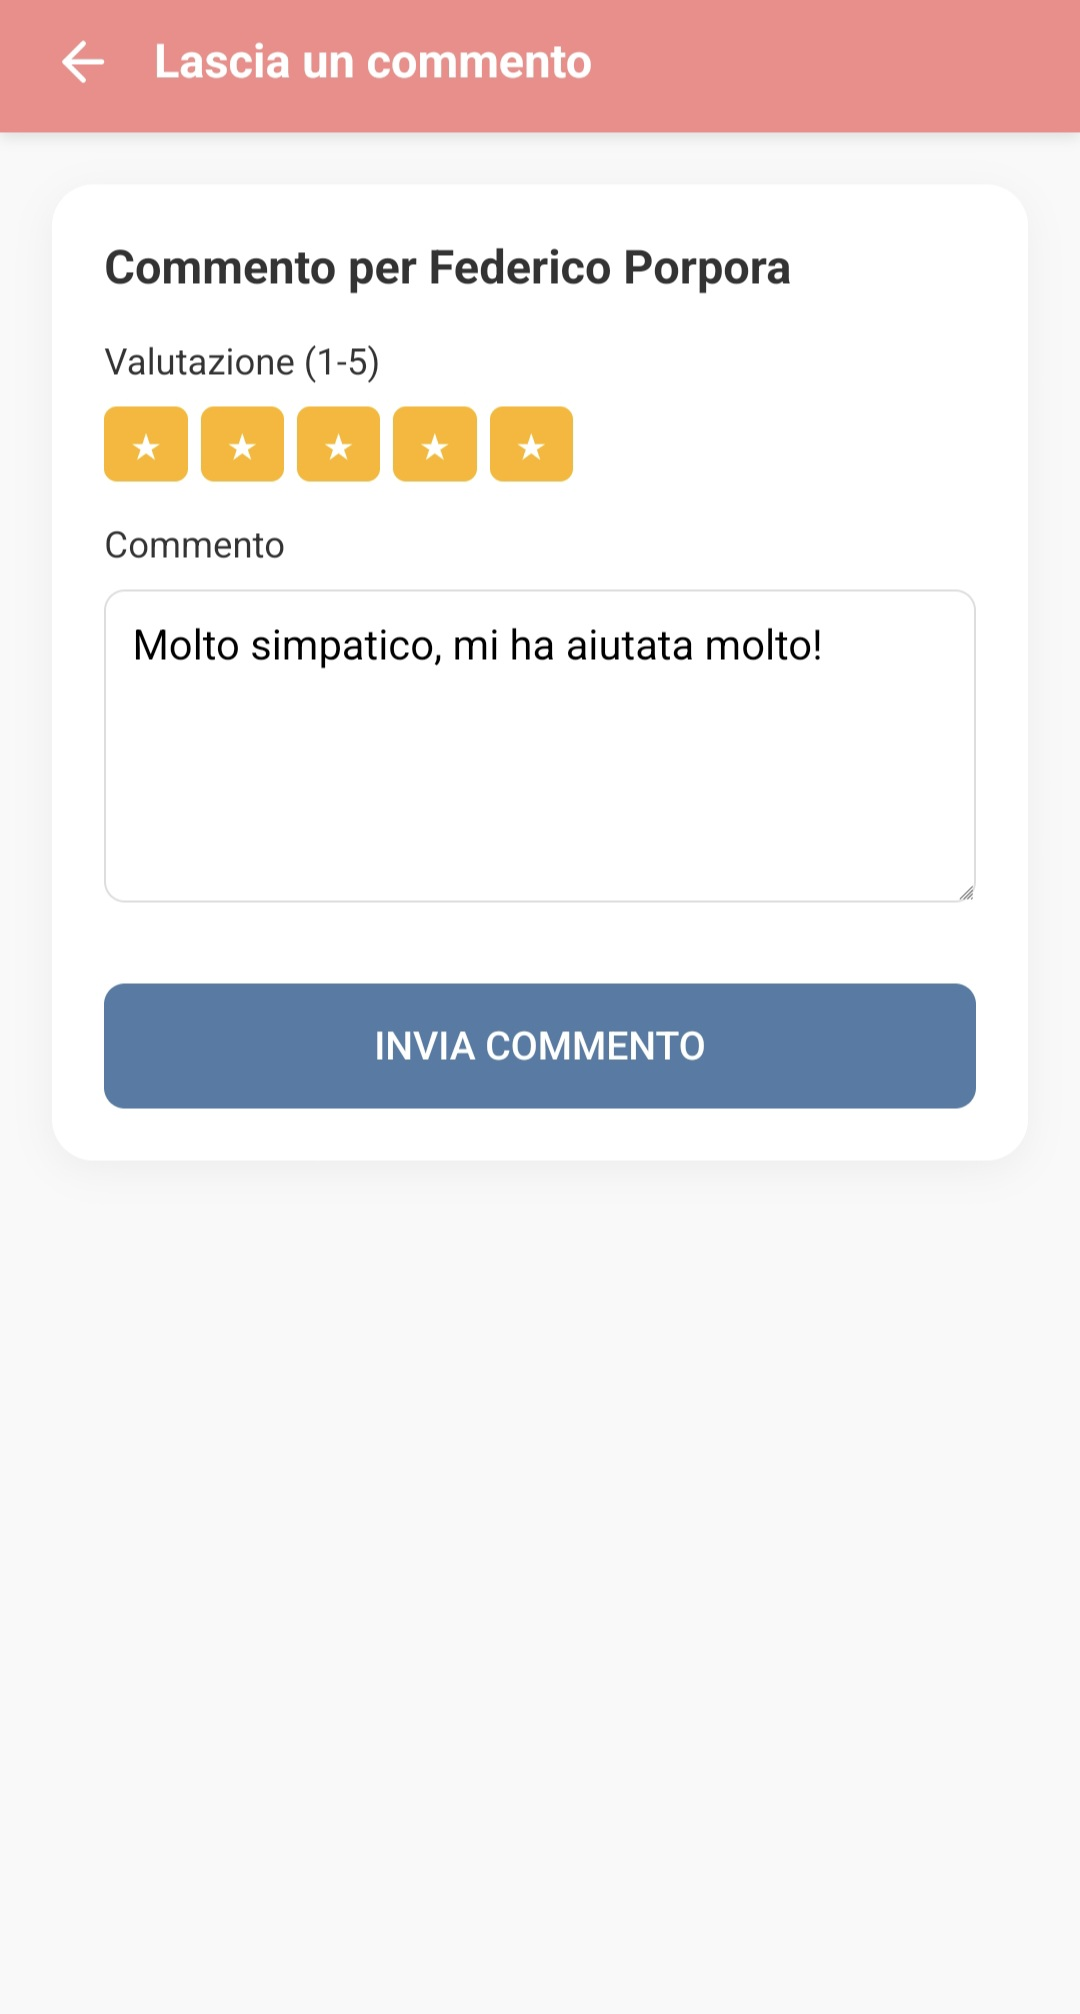
\includegraphics[width=0.98\linewidth,height=0.30\textheight,keepaspectratio]{images/commento.jpg}}
        \caption{Aggiunta Commento}
    \end{minipage}
\end{figure}


% Progettazione della persistenza
\newpage
\section{Progettazione della persistenza}
Di seguito è riportato il diagramma ER della persistenza del sistema.

\begin{figure}[H]
    \centering
    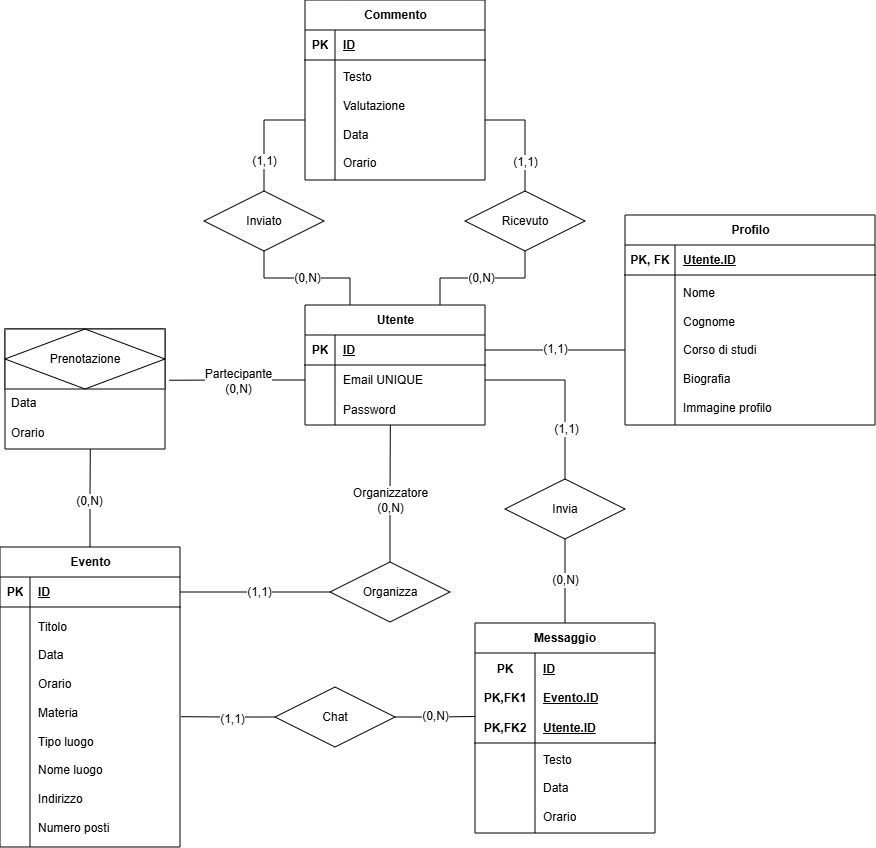
\includegraphics[width=\textwidth,height=0.5\textheight,keepaspectratio]{images/diagramma-entity-relationship.png}
    \caption{Diagramma Entity-Relationship}
\end{figure}
%
È da notare che:
\begin{itemize}[leftmargin=*]
    \item \textbf{Separazione tra autenticazione e profilo (1:1)}: L'entità \texttt{Profilo} è separata da \texttt{Utente} tramite una relazione uno-a-uno, in cui la chiave primaria di \texttt{Profilo} funge contemporaneamente da chiave esterna riferita a \texttt{Utente.ID}. Questo evita di sovraccaricare la tabella delle credenziali con dati personali e pesanti (come l'immagine di profilo), ottimizzando le operazioni di autenticazione.
    \item \textbf{Doppia relazione Utente-Commento}: L'entità \texttt{Commento} è legata a \texttt{Utente} attraverso due relazioni distinte: \texttt{Inviato} (lo studente autore del commento) e \texttt{Ricevuto} (lo studente che riceve la recensione). Questa struttura consente di implementare un sistema di feedback bidirezionale chiaro, tracciando univocamente mittente e destinatario.
    \item \textbf{Prenotazione come entità associativa}: La partecipazione degli utenti agli eventi è gestita tramite la relazione molti-a-molti \texttt{Prenotazione}, arricchita dagli attributi \texttt{Data} e \texttt{Orario}. Questo consente di memorizzare non solo l'associazione tra utente ed evento, ma anche il momento esatto in cui è avvenuta la prenotazione.
    \item \textbf{Messaggistica e vincolo di contesto}: L'entità \texttt{Messaggio} ha una chiave primaria composta che include le chiavi esterne riferite sia a \texttt{Evento} (\texttt{Evento.ID}) sia a \texttt{Utente} (\texttt{Utente.ID}). Ciò assicura l'integrità referenziale, legando indissolubilmente ogni messaggio alla specifica chat dell'evento e all'utente che lo ha inviato.
\end{itemize}







% Progettazione del collaudo
\newpage
\section{Progettazione del collaudo}
Il collaudo è effettuato attraverso sistemi di testing automatici eseguiti sulle
modifiche del codice (\emph{continuous integration}). I test sono divisi in tre
categorie a seconda di ciò che vanno a verificare:
\begin{itemize}
    \item \textbf{Test di unità}: controllano il comportamento dei singoli componenti;
    \item \textbf{Test di integrazione}: controllano le interazioni tra i vari componenti;
    \item \textbf{Test punto a punto}: controllano il funzionamento del sistema nel suo
          complesso.
\end{itemize}
Coerentemente con il Piano del collaudo (Sezione 2.9), sono presentati
solo i test di unità delle classi ritenute centrali per il funzionamento del sistema,
riallineati alla struttura emersa dalla Progettazione di dettaglio (Sezione 3.2).

In particolare, rispetto all'analisi, l'entità \texttt{Profilo} è stata scomposta
nelle classi \texttt{Account}, \texttt{Utente} e \texttt{ProfiloUtente}, le entità
\texttt{CommentoInviato} e \texttt{CommentoRicevuto} sono state unificate nella
singola classe \texttt{Commento}, mentre l'\texttt{Evento} si specializza in
\texttt{EventoAPostiLimitati} ed \texttt{EventoAPostiIllimitati}. Vengono presentati
i test di unità di Evento e Profilo.

\subsection{Test di unità: Evento}
\begin{lstlisting}
using NUnit.Framework;

[TestFixture]
public class TestEvento
{
    private EventoAPostiLimitati eventoLimitato;
    private EventoAPostiIllimitati eventoIllimitato;
    private Utente organizzatore;
    private Luogo luogoPubblico, luogoPrivato;

    [SetUp]
    public void Setup()
    {
        organizzatore = new Utente(
            "matteo.gattobigio@studio.unibo.it",
            "Password1!",
            new ProfiloUtente(
                "Matteo", "Gattobigio",
                "Ingegneria Informatica", "Studente appassionato e vivace",
                null
            )
        );

        luogoPubblico = new Luogo(
            "Biblioteca Universitaria",
            "Via Zamboni 33",
            TipoDiLuogo.Pubblico
        );

        luogoPrivato = new Luogo(
            "Appartamento studio",
            "Via Irnerio 12",
            TipoDiLuogo.Privato
        );

        eventoLimitato = new EventoAPostiLimitati(
            "Studio Analisi II",
            new DateTime(2026, 7, 15, 14, 0, 0),
            luogoPubblico,
            organizzatore,
            2
        );

        eventoIllimitato = new EventoAPostiIllimitati(
            "Ripasso Reti di Calcolatori",
            new DateTime(2026, 7, 20, 10, 0, 0),
            luogoPrivato,
            organizzatore
        );
    }

    [Test]
    public void TestCreazioneEvento()
    {
        Assert.AreEqual("Studio Analisi II",
            eventoLimitato.getTitolo());
        Assert.AreEqual(new DateTime(2026, 7, 15, 14, 0, 0),
            eventoLimitato.getDataEOrario());
        Assert.AreEqual(luogoPubblico,
            eventoLimitato.getLuogo());
        Assert.AreEqual(organizzatore,
            eventoLimitato.getOrganizzatore());
        Assert.AreEqual(2,
            eventoLimitato.getPosti());
        Assert.IsTrue(eventoLimitato.getLuogo().isPubblico());
    }

    [Test]
    public void TestEventoIllimitato()
    {
        Assert.AreEqual("Ripasso Reti di Calcolatori",
            eventoIllimitato.getTitolo());
        Assert.AreEqual(luogoPrivato,
            eventoIllimitato.getLuogo());
        Assert.IsTrue(eventoIllimitato.getLuogo().isPrivato());
    }

    [Test]
    public void TestAggiungiPartecipante()
    {
        Utente partecipante = new Utente(
            "federico.porpora@studio.unibo.it",
            "Password1!",
            new ProfiloUtente(
                "Federico", "Porpora",
                "Ingegneria Informatica", "Studio volentieri in gruppo",
                null
            )
        );

        eventoLimitato.aggiungiPartecipante(partecipante);

        CollectionAssert.Contains(
            eventoLimitato.getPartecipanti(),
            partecipante
        );
        Assert.AreEqual(1,
            eventoLimitato.getPartecipanti().Count);
    }

    [Test]
    public void TestRimozionePartecipante()
    {
        Utente partecipante = new Utente(
            "federico.porpora@studio.unibo.it",
            "Password1!",
            new ProfiloUtente(
                "Federico", "Porpora",
                "Ingegneria Informatica", "Studio volentieri in gruppo",
                null
            )
        );

        eventoLimitato.aggiungiPartecipante(partecipante);
        eventoLimitato.rimuoviPartecipante(partecipante);

        CollectionAssert.DoesNotContain(
            eventoLimitato.getPartecipanti(),
            partecipante
        );
        Assert.AreEqual(0,
            eventoLimitato.getPartecipanti().Count);
    }

    [Test]
    public void TestPuoPartecipare()
    {
        Utente lucilla = new Utente(
            "lucilla.lucchi@studio.unibo.it", "Password1!",
            new ProfiloUtente(
                "Lucilla", "Lucchi",
                "Ingegneria Informatica", "Studio bene quando faccio tante pause",
                null
            )
        );
        Utente p2 = new Utente(
            "anna.verdi@studio.unibo.it", "Password1!",
            new ProfiloUtente("Anna", "Verdi", "Matematica", "", null)
        );
        Utente p3 = new Utente(
            "sara.neri@studio.unibo.it", "Password1!",
            new ProfiloUtente("Sara", "Neri", "Fisica", "", null)
        );

        // Evento a posti limitati (2 posti): si riempie
        Assert.IsTrue(eventoLimitato.puoPartecipare(lucilla));
        eventoLimitato.aggiungiPartecipante(lucilla);
        eventoLimitato.aggiungiPartecipante(p2);
        Assert.IsFalse(eventoLimitato.puoPartecipare(p3));

        // Evento a posti illimitati: accetta sempre
        eventoIllimitato.aggiungiPartecipante(lucilla);
        eventoIllimitato.aggiungiPartecipante(p2);
        eventoIllimitato.aggiungiPartecipante(p3);
        Assert.IsTrue(eventoIllimitato.puoPartecipare(
            new Utente(
                "extra@studio.unibo.it", "Password1!",
                new ProfiloUtente("Extra", "Utente", "Chimica", "", null)
            )
        ));
    }

    [Test]
    public void TestChatGenerata()
    {
        Assert.IsNotNull(eventoLimitato.getChat());
    }
}
\end{lstlisting}

\subsection{Test di unità: Profilo}
\begin{lstlisting}
using NUnit.Framework;

[TestFixture]
public class TestProfilo
{
    private ProfiloUtente profiloCompleto, profiloMinimo;
    private Utente utente;

    [SetUp]
    public void Setup()
    {
        profiloCompleto = new ProfiloUtente(
            "Federico", "Porpora",
            "Ingegneria Informatica",
            "Studio volentieri in gruppo",
            "immagine.png"
        );

        profiloMinimo = new ProfiloUtente(
            "Luca", "Bianchi",
            "Matematica",
            "",
            null
        );

        utente = new Utente(
            "federico.porpora@studio.unibo.it",
            "Password1!",
            profiloCompleto
        );
    }

    [Test]
    public void TestCreazioneProfilo()
    {
        Assert.AreEqual("Federico",
            profiloCompleto.getNome());
        Assert.AreEqual("Porpora",
            profiloCompleto.getCognome());
        Assert.AreEqual("Ingegneria Informatica",
            profiloCompleto.getCorsoDiStudi());
        Assert.AreEqual("Studio volentieri in gruppo",
            profiloCompleto.getBiografia());
        Assert.AreEqual("immagine.png",
            profiloCompleto.getImmagine());
    }

    [Test]
    public void TestProfiloMinimo()
    {
        Assert.AreEqual("Luca",
            profiloMinimo.getNome());
        Assert.AreEqual("Bianchi",
            profiloMinimo.getCognome());
        Assert.AreEqual("Matematica",
            profiloMinimo.getCorsoDiStudi());
        Assert.AreEqual("",
            profiloMinimo.getBiografia());
        Assert.IsNull(profiloMinimo.getImmagine());
    }

    [Test]
    public void TestSetterProfilo()
    {
        profiloCompleto.setNome("Giuseppe");
        Assert.AreEqual("Giuseppe",
            profiloCompleto.getNome());

        profiloCompleto.setCognome("Verdi");
        Assert.AreEqual("Verdi",
            profiloCompleto.getCognome());

        profiloCompleto.setCorsoDiStudi("Fisica");
        Assert.AreEqual("Fisica",
            profiloCompleto.getCorsoDiStudi());

        profiloCompleto.setBiografia("Nuova biografia");
        Assert.AreEqual("Nuova biografia",
            profiloCompleto.getBiografia());

        profiloCompleto.setImmagine("nuova_immagine.png");
        Assert.AreEqual("nuova_immagine.png",
            profiloCompleto.getImmagine());
    }

    [Test]
    public void TestCreazioneUtente()
    {
        Assert.AreEqual("federico.porpora@studio.unibo.it",
            utente.getEmail());
        Assert.AreEqual(profiloCompleto,
            utente.getProfiloUtente());
        Assert.AreEqual(0,
            utente.getCommentiRicevuti().Count);
    }

    [Test]
    public void TestCommenti()
    {
        Utente autore = new Utente(
            "luca.bianchi@studio.unibo.it",
            "Password1!",
            profiloMinimo
        );

        Commento commento = new Commento(
            autore,
            "Ottimo compagno di studio",
            4,
            new DateTime(2026, 7, 16, 18, 0, 0)
        );

        utente.aggiungiCommento(commento);

        CollectionAssert.Contains(
            utente.getCommentiRicevuti(),
            commento
        );
        Assert.AreEqual(1,
            utente.getCommentiRicevuti().Count);
        Assert.AreEqual(4,
            commento.getValutazione());
        Assert.AreEqual(autore,
            commento.getAutore());
    }
}
\end{lstlisting}



% Progettazione del deployment
\newpage
\section{Progettazione del deployment}
Il deployment dell'applicazione sarà così gestito:
\begin{itemize}[leftmargin=*]
    \item La parte server del programma sarà installata su un server fisico. Per favorire l'eventuale espansione orizzontale del sistema, il processo sarà automatizzato tramite Docker. Il server sarà composto da:
    \begin{itemize}[leftmargin=*]
        \item Il server web che si occupa della gestione delle richieste REST in arrivo, sviluppato in ambiente .NET;
        \item Un DBMS (PostgreSQL) con cui il server web interagirà per la gestione della persistenza.
    \end{itemize}
    \item La parte client sarà fornita da un server web che servirà l'applicazione frontend sviluppata tramite Vite. Non richiede particolari azioni da parte dell'utente finale, che potrà accedere all'interfaccia tramite un comune browser.
\end{itemize}

\subsection{Artefatti}
L'applicazione è divisa in due artefatti principali:
\begin{itemize}[leftmargin=*]
    \item Il software che compone il \textbf{backend}, che implementa la logica di business, il livello di traduzione REST e la gestione della persistenza;
    \item Il software che compone il \textbf{frontend}, che implementa le view e il livello di traduzione tra l'interfaccia dell'Utente e le chiamate HTTP dirette al backend.
\end{itemize}
\begin{figure}[H]
    \centering
    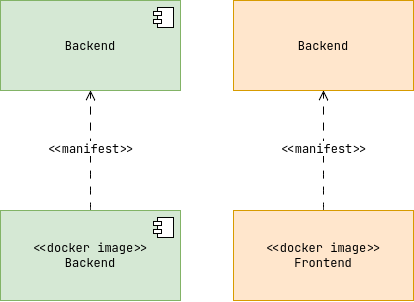
\includegraphics[width=0.5\textwidth,height=0.5\textheight,keepaspectratio]{images/diagramma-degli-artefatti.png}
    \caption{Diagramma degli artefatti}
\end{figure}
%
Questi artefatti racchiudono tutti i package definiti in fase di analisi e progettazione, fornendo all'Utente le funzionalità per agire sia come Organizzatore che come Partecipante.

\subsection{Target di deploy}
In linea con le scelte architetturali, l'applicazione sarà \textit{web-based}, di conseguenza il deploy è diviso in due sezioni:
\begin{itemize}[leftmargin=*]
    \item Il deploy del \textbf{backend} verrà effettuato inizialmente su un singolo nodo, ma sarà eseguito con strumenti di automazione come Docker per favorire una futura espansione orizzontale, con l'eventuale necessità di load balancer.
    \item Il deploy del \textbf{frontend} verrà eseguito analogamente al backend, servito su più nodi indipendenti o piattaforme specializzate il cui compito è distribuire il software ai browser web dei clienti.
\end{itemize}

I programmi sul server saranno eseguiti da utenti del sistema con permessi minimi, in modo da garantire la sicurezza del nodo contro eventuali attacchi. Le credenziali per il database (PostgreSQL) e le chiavi segrete per l'autenticazione JWT verranno iniettate a livello di deployment tramite variabili d'ambiente in modo da essere facilmente modificabili.
Di seguito sono presentati i due possibili scenari di deploy:
\begin{itemize}[leftmargin=*]
    \item Uno schema base con un singolo nodo che gestisce i container del frontend, del backend e del database (più semplice per lo sviluppo e il testing);
\end{itemize}
    \begin{figure}[H]
        \centering
        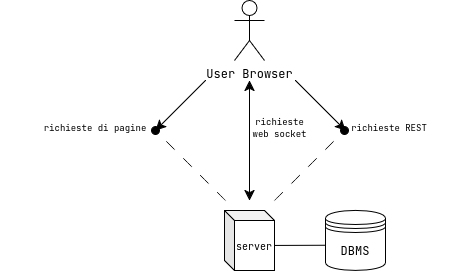
\includegraphics[width=0.5\textwidth,height=0.5\textheight,keepaspectratio]{images/deploy-base.png}
        \caption{Deploy: Schema base}
    \end{figure}
%
\begin{itemize}[leftmargin=*]
    \item Uno schema scalabile orizzontalmente, dove i target sono configurati in automatico tramite orchestratori (es. Docker) e un reverse proxy gestisce il bilanciamento del carico tra i vari nodi REST.
    \begin{figure}[H]
        \centering
        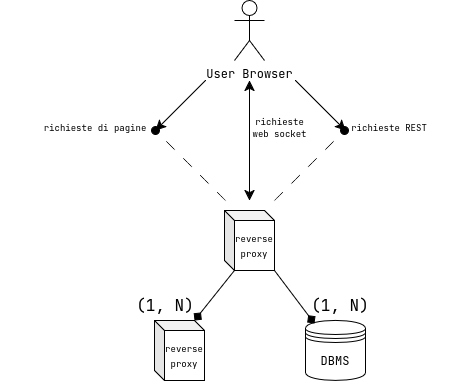
\includegraphics[width=0.5\textwidth,height=0.5\textheight,keepaspectratio]{images/deploy-scalabile.png}
        \caption{Deploy: Schema scalabile}
    \end{figure}
%
\end{itemize}

\end{document}